% Options for packages loaded elsewhere
\PassOptionsToPackage{unicode}{hyperref}
\PassOptionsToPackage{hyphens}{url}
\PassOptionsToPackage{dvipsnames,svgnames,x11names}{xcolor}
\documentclass[
  12pt,
]{article}
\usepackage{xcolor}
\usepackage[margin=1in]{geometry}
\usepackage{amsmath,amssymb}
\setcounter{secnumdepth}{-\maxdimen} % remove section numbering
\usepackage{iftex}
\ifPDFTeX
  \usepackage[T1]{fontenc}
  \usepackage[utf8]{inputenc}
  \usepackage{textcomp} % provide euro and other symbols
\else % if luatex or xetex
  \usepackage{unicode-math} % this also loads fontspec
  \defaultfontfeatures{Scale=MatchLowercase}
  \defaultfontfeatures[\rmfamily]{Ligatures=TeX,Scale=1}
\fi
\usepackage[]{newtxtext}
\ifPDFTeX\else
  % xetex/luatex font selection
\fi
% Use upquote if available, for straight quotes in verbatim environments
\IfFileExists{upquote.sty}{\usepackage{upquote}}{}
\IfFileExists{microtype.sty}{% use microtype if available
  \usepackage[]{microtype}
  \UseMicrotypeSet[protrusion]{basicmath} % disable protrusion for tt fonts
}{}
\usepackage{setspace}
\makeatletter
\@ifundefined{KOMAClassName}{% if non-KOMA class
  \IfFileExists{parskip.sty}{%
    \usepackage{parskip}
  }{% else
    \setlength{\parindent}{0pt}
    \setlength{\parskip}{6pt plus 2pt minus 1pt}}
}{% if KOMA class
  \KOMAoptions{parskip=half}}
\makeatother
% definitions for citeproc citations
\NewDocumentCommand\citeproctext{}{}
\NewDocumentCommand\citeproc{mm}{%
  \begingroup\def\citeproctext{#2}\cite{#1}\endgroup}
\makeatletter
 % allow citations to break across lines
 \let\@cite@ofmt\@firstofone
 % avoid brackets around text for \cite:
 \def\@biblabel#1{}
 \def\@cite#1#2{{#1\if@tempswa , #2\fi}}
\makeatother
\newlength{\cslhangindent}
\setlength{\cslhangindent}{1.5em}
\newlength{\csllabelwidth}
\setlength{\csllabelwidth}{3em}
\newenvironment{CSLReferences}[2] % #1 hanging-indent, #2 entry-spacing
 {\begin{list}{}{%
  \setlength{\itemindent}{0pt}
  \setlength{\leftmargin}{0pt}
  \setlength{\parsep}{0pt}
  % turn on hanging indent if param 1 is 1
  \ifodd #1
   \setlength{\leftmargin}{\cslhangindent}
   \setlength{\itemindent}{-1\cslhangindent}
  \fi
  % set entry spacing
  \setlength{\itemsep}{#2\baselineskip}}}
 {\end{list}}
\usepackage{calc}
\newcommand{\CSLBlock}[1]{\hfill\break\parbox[t]{\linewidth}{\strut\ignorespaces#1\strut}}
\newcommand{\CSLLeftMargin}[1]{\parbox[t]{\csllabelwidth}{\strut#1\strut}}
\newcommand{\CSLRightInline}[1]{\parbox[t]{\linewidth - \csllabelwidth}{\strut#1\strut}}
\newcommand{\CSLIndent}[1]{\hspace{\cslhangindent}#1}
\setlength{\emergencystretch}{3em} % prevent overfull lines
\providecommand{\tightlist}{%
  \setlength{\itemsep}{0pt}\setlength{\parskip}{0pt}}
\usepackage{amsmath,amssymb,amsthm}
\usepackage{newtxmath}
\usepackage{booktabs}
\usepackage{threeparttable}
\usepackage{graphicx}
\usepackage{float}
\usepackage{pdflscape}
\usepackage{needspace}
\usepackage{setspace}
\usepackage{etoolbox}
\usepackage[font=small,labelfont=bf,labelsep=period]{caption}
\usepackage[section]{placeins}
\definecolor{paperlink}{RGB}{31,59,115}
\allowdisplaybreaks
\setlength{\parskip}{0pt}
\setlength{\parindent}{1.5em}
\AtBeginEnvironment{CSLReferences}{\interlinepenalty=10000}
\AfterEndEnvironment{abstract}{\clearpage}
\usepackage{bookmark}
\IfFileExists{xurl.sty}{\usepackage{xurl}}{} % add URL line breaks if available
\urlstyle{same}
\hypersetup{
  pdftitle={Competition Creates Competition: Stock Prices and the Discovery of Takeover Bidders},
  pdfauthor={Austin Li},
  colorlinks=true,
  linkcolor={paperlink},
  filecolor={Maroon},
  citecolor={paperlink},
  urlcolor={paperlink},
  pdfcreator={LaTeX via pandoc}}

\ifXeTeX
\special{pdf:trailerid [ <da68b6cc703ee430b424c0b4bbec075a> <da68b6cc703ee430b424c0b4bbec075a> ]}
\fi
\ifPDFTeX
\pdftrailerid{}
\pdftrailer{/ID [ <da68b6cc703ee430b424c0b4bbec075a> <da68b6cc703ee430b424c0b4bbec075a> ]}
\fi
\ifLuaTeX
\pdfvariable trailerid {[ <da68b6cc703ee430b424c0b4bbec075a> <da68b6cc703ee430b424c0b4bbec075a> ]}
\fi

\title{Competition Creates Competition: Stock Prices and the Discovery
of Takeover Bidders}
\author{Austin Li}
\date{}

\begin{document}
\maketitle
\begin{abstract}
A stronger incumbent bidder can attract a challenger by making the
target's stock price more informative. I study a takeover auction in
which a prospective buyer sees the price before it pays to prepare a
bid. A stronger incumbent lowers the buyer's acquisition profit at
every belief about its quality. It also makes the proceeds of target
shareholders more sensitive to that quality. An investor who knows the
buyer's quality class therefore gains more from trading on it. For a
set of parameters with positive measure, a stronger incumbent turns an
uninformative price into an informative one. In each economy the
trading and preparation outcomes are unique. Challenger participation
rises, and so does the probability that a challenger from the
high-value class acquires the target. If the information in the price
is held fixed, stronger competition lowers participation. The reversal
also holds when the buyer has a more accurate private signal than the
investor. In the strong-incumbent economy, access to prices raises
expected target proceeds and acquisition surplus net of preparation
costs.
\end{abstract}

\setstretch{2}
\section{1. Introduction}\label{sec-introduction}

At fixed information, a stronger incumbent reduces a prospective
challenger's expected return from entering a takeover contest. The
challenger must pay preparation costs before it can submit an executable
offer, and a stronger rival lowers what that preparation earns
(\citeproc{ref-Fishman1988}{Fishman 1988};
\citeproc{ref-HirshleiferPng1989}{Hirshleifer and Png 1989}). I study a
force in the opposite direction. Competition can make the target's stock
more informative about the challenger. When a potential buyer observes
that price before committing to acquisition preparation, the information
effect can outweigh the loss of acquisition profits. A stronger
incumbent then attracts a competing buyer and raises the probability
that a challenger from the high-value class acquires the target.

The setting is a listed target with a public sale opportunity. One buyer is already prepared, and another has not committed to the diligence that an executable proposal requires; \hyperref[sec-the-decision-interval]{Section 2.1} describes the decision interval in which that buyer decides while the target's stock trades. Incumbent strength is the public distribution of the prepared bidder's value; a stronger incumbent shifts it upward, and no offer is announced before the challenger decides.

The mechanism runs through two claims on the same acquisition surplus.
The challenger holds the acquisition claim, what it keeps if it
prepares, bids, and wins. Target shareholders hold the traded claim,
what the auction pays them. The challenger's value comes from a
high-value or a low-value quality class. Each bidder bids its value in
the cash second-price auction. A prepared challenger's value then goes
to the two claims: a win splits it into the payment and the profit, and
a loss makes the winning incumbent pay the challenger's bid. The
expected value gap between the classes is fixed by the classes alone.
A stronger incumbent changes only who receives it. It outbids the
challenger more often and pays the challenger's bid, so more of the gap
reaches target proceeds. A winning challenger pays more, so less of
the gap remains as acquisition profit, at every belief. Target shares become
more sensitive to information about the challenger at the same time as
the challenger's own return to preparation falls. An investor who knows
the challenger's class trades on that sensitivity against noise demand.
Competitive market makers price order flow and anticipate the
preparation that each price will induce, but noise leaves the investor a
residual advantage. A larger gap in target proceeds can make that
advantage worth the cost of trading.

The informed investor is an outside specialist with no net position in
the target. Its information is the challenger's quality class. Target
shareholders gain when the price recruits entry, because a holder
through the sale receives sale proceeds, not the interim price.

The main result compares a weak-incumbent economy with a
strong-incumbent economy on a nonempty open set of primitives. In each
economy the trading outcome and the on-path preparation outcome are
unique. With the weak incumbent, the investor's residual advantage
cannot cover trading costs, the price reveals nothing, and only a
zero-cost challenger prepares. With the strong incumbent, informed
trading pays, the investor trades to its limit, and favorable prices
bring in a high-cost challenger. Preparation rises even though
acquisition profit falls at every fixed belief, and the probability that
a challenger from the high-value class owns the target rises with it. Market makers anticipate the preparation each price induces, so the reversal holds under rational pricing. Uniqueness allows arbitrary mixed orders and every unilateral deviation to an order in \([-1,1]\); a global bound on marginal trading profit covers them all. The change in information does the
work. If the investor's orders are held fixed at their informative level
while the incumbent strengthens, preparation falls, as the
fixed-information benchmark predicts.

The reversal holds at some incumbent strengths and costs for every prior and every pair of classes that differ above the reserve, when the high class has stochastically higher values and both class supports lie above the reserve. Dispersion within a class raises the option value of preparation: in an example in \hyperref[sec-acquisition-values]{Section 5.2}, dispersed classes produce the reversal and point-mass classes with the same means, costs, prior, and strengths do not. The reversal also holds for every noise law whose score bound is below one (\hyperref[result-proposition-a-5]{Proposition A.5}). At a given bound, Laplace noise gives the most informative flow experiment at every pure order profile. The size of the effect depends on the noise law: in the strong benchmark economy, entry is 0.522757 under Laplace noise and 0.301509 under logistic noise, against a floor of 0.250000 (\hyperref[sec-noise-and-preparation-costs]{Section 5.1}). The reversal survives atomless preparation costs and private signals that the buyer and the investor hold about different facts, including a buyer signal more accurate than the investor's. At some intermediate incumbent strengths, informative and uninformative equilibria coexist: a computer-assisted proof establishes three informative equilibria, with preparation strictly ordered upward across them. Against a strong enough incumbent, even the most favorable feasible price cannot justify expensive preparation, so participation returns to its floor while trading stays informative; participation is therefore non-monotone in strength. In the strong-incumbent economy, access to prices raises expected target proceeds and acquisition surplus net of preparation costs.

Sale terms shape both what a winning buyer pays and what the stock price can reveal before anyone prepares. A reserve that excludes the low-value class, for instance, can support informative trading against an incumbent that would otherwise leave the price uninformative. I compare two reserves at which the trading outcome is unique. An alternative bargaining institution shows that the effect of competition on the target-payoff spread depends on the weight the payment rule places on the runner-up's value.

The paper belongs to the literature on the real effects of financial markets (\citeproc{ref-BondEdmansGoldstein2012}{Bond et al. 2012}). The closest antecedent is Dow et al. (\citeproc{ref-DowGoldsteinGuembel2017}{2017}), where a firm's investment decision feeds back into the incentive to produce information about its stock. Here the sale rule divides acquisition surplus between a traded claim and a buyer that decides whether to participate. Edmans et al. (\citeproc{ref-EdmansGoldsteinJiang2015}{2015}) show that corrective real decisions can discourage trading on bad news under rational pricing; here the real decision is the buyer's participation itself. Firms learn from peers' stock prices (\citeproc{ref-FoucaultFresard2014}{Foucault and Fr\'esard 2014}), and target prices affect takeover activity (\citeproc{ref-EdmansGoldsteinJiang2012}{Edmans et al. 2012}); in this model a prospective challenger learns about its own acquisition value from the target's price before it commits. Learning from announcement returns in completion decisions (\citeproc{ref-Luo2005}{Luo 2005}) occurs after this participation margin.

The auction-entry literature makes the bidder pool endogenous (\citeproc{ref-Samuelson1985}{Samuelson 1985}; \citeproc{ref-McAfeeMcMillan1987}{McAfee and McMillan 1987}; \citeproc{ref-LevinSmith1994}{Levin and Smith 1994}; \citeproc{ref-GentryStroup2019}{Gentry and Stroup 2019}) and shows how selective entry affects the choice of sale procedure (\citeproc{ref-RobertsSweeting2013}{Roberts and Sweeting 2013}). The challenger here faces selective entry in the terms of that literature. Its pre-entry information indexes the distribution of its value, and paying the entry cost reveals the value (\citeproc{ref-MarmerShneyerovXu2013}{Marmer et al. 2013}; \citeproc{ref-GentryLi2014}{Gentry and Li 2014}; \citeproc{ref-RobertsSweeting2013}{Roberts and Sweeting 2013}). The two limits of this framework are a bidder that knows only the common value distribution before entry (\citeproc{ref-LevinSmith1994}{Levin and Smith 1994}) and a bidder that already knows its value (\citeproc{ref-Samuelson1985}{Samuelson 1985}). Here the pre-entry information is the target's stock price, which is public and moves with the orders of an investor who observes the challenger's quality class. I keep the direct deterrence force of that literature and add a market that operates before preparation. Auction formats also affect bidders' incentives to acquire information (\citeproc{ref-Persico2000}{Persico 2000}); the informed trader here is outside the auction and trades a payoff that differs from the entrant's profit. Recent work studies bidder learning about own values and competitors (\citeproc{ref-PernoudGleyze2026}{Pernoud and Gleyze 2026}). It also studies post-auction feedback in security-payment design (\citeproc{ref-LiuBernhardt2022}{Liu and Bernhardt 2022}) and bidder-pool choice with correlated values (\citeproc{ref-CarlinEtAl2026}{Carlin et al. 2026}).

In takeovers, Betton et al. (\citeproc{ref-BettonEtAl2014}{2014}) study negotiations with stock-market feedback, and Lin et al. (\citeproc{ref-LinMaYangZhu2025}{2025}) model payment choice and trading within an initiated deal; I hold cash consideration fixed and study entry. Arbitrageurs' positions can affect tendering (\citeproc{ref-CornelliLi2002}{Cornelli and Li 2002}); the investor here has information about a prospective acquirer and no role in tendering. The model abstracts from toeholds and dispersed-shareholder free riding (\citeproc{ref-BulowHuangKlemperer1999}{Bulow et al. 1999}; \citeproc{ref-GrossmanHart1980}{Grossman and Hart 1980}) and takes the investor's information as given. Endogenous research would add manipulation through the real decision that responds to the price (\citeproc{ref-GoldsteinGuembel2008}{Goldstein and Guembel 2008}).
An informed trader can also hold a stake before a control decision.
Noise then lets an acquirer conceal share purchases before a bid
(\citeproc{ref-KyleVila1991}{Kyle and Vila 1991}). Large holders trade
on their information (\citeproc{ref-Edmans2009}{Edmans 2009}), monitor,
or intervene as prices feed back to firm decisions
(\citeproc{ref-EdmansGoldsteinJiang2015}{Edmans et al. 2015},
Section II.E; \citeproc{ref-Maug1998}{Maug 1998};
\citeproc{ref-BackEtAl2018}{Back et al. 2018}). The baseline investor
in this paper holds no stake, seeks no control, and earns only the
trading residual; a stake enters only as an extension (Online Appendix
A.12).

\hyperref[sec-model]{Section 2} describes the decision interval and sets out the model.
\hyperref[sec-payoffs]{Section 3} derives the two returns to information
and what the challenger can learn from the price.
\hyperref[sec-results]{Section 4} states the main result, the
fixed-experiment control, and the coexisting equilibria.
\hyperref[sec-extensions]{Section 5} covers robustness and complementary
private information, \hyperref[sec-welfare]{Section 6} welfare and sale
terms, and \hyperref[sec-program]{Section 7} empirical implications.
\hyperref[sec-conclusion]{Section 8} concludes.
\hyperref[paper-appendix]{Appendix A} contains supporting results and
proofs; the Online Appendix contains the measure-theoretic arguments, the numerical methods, and the replication files.

\section{2. The model}\label{sec-model}

\subsection{2.1 The decision interval}\label{sec-the-decision-interval}

The model applies to a listed target whose sale opportunity is publicly
understood while its stock still trades and while a further bidder can
still come in. A disclosed approach, an announced strategic review, or an open contest can create such an interval if the opportunity becomes public before the buyer set is fixed; only then can a prospective buyer watch the price during the period that matters. Whether a given transaction fits is a question about its chronology, and Online Appendix D shows how to establish that chronology from disclosure records.

Within the interval, one buyer is already prepared. It may be the
approaching party or a bidder that has completed diligence, and its
strength is what the public can infer about its acquisition value from
the disclosed record. Another buyer has not decided whether to prepare.
Preparation is required for an executable proposal. Before a buyer can
submit a binding offer it must verify the target's contracts,
liabilities, and technology, arrange financing and approvals, and commit
evaluation capacity that has other uses. Those costs are sunk once
incurred, and they differ across buyers. Prior familiarity, existing
capacity, or a small deal relative to the buyer's size make preparation
cheap for some buyers and expensive for others. A buyer that declines to
prepare cannot bid its current expected value instead; it stays out. The
challenger's cost is a participation cost, not the price of an optional
report.

The investor and the buyer know different things. A buyer knows its own integration plans. A specialist investor may know what the
target's customers are doing, how its technology compares with
alternatives, or where its product demand is heading. These are different facts about the same acquisition match, so a more accurate signal about one can leave the other unknown. The model suppresses
the buyer's initial information and gives the investor exact knowledge
of the challenger's quality class, though not of its value, so that the
mechanism is easy to see;
\hyperref[sec-complementary-private-information]{Section 5.3} removes
both extremes. The identity of the natural further buyer is common
knowledge within the interval. What the market does not know is how
well that buyer fits the target.

Public incumbent strength is a distribution, not a bid. The record can
reveal that a strategic acquirer with clear synergies is at the table,
or that the prepared party is a financial buyer with a leveraged capital structure, without revealing what either would pay; strategic and financial bidders differ systematically in their valuations (\citeproc{ref-GorbenkoMalenko2014}{Gorbenko and Malenko 2014}). The model varies
that distribution and keeps the incumbent's realized value private until
it bids.

Disclosure records support the stage structure. Imprivata's definitive proxy
separates an unsolicited approach, outreach to potential buyers, and
indications of interest conditional on further diligence
(\citeproc{ref-Imprivata2016}{Imprivata, Inc. 2016}), and takeover
competition develops before public bidding more generally
(\citeproc{ref-BooneMulherin2007}{Boone and Mulherin 2007};
\citeproc{ref-GentryStroup2019}{Gentry and Stroup 2019}). These records document a costly preparation stage; \hyperref[sec-program]{Section 7} states how to test whether prices draw buyers into it.

\subsection{2.2 Values, preparation, and the
sale}\label{sec-values-preparation-and-the-sale}

The target's known standalone value is normalized to zero. Acquisition
values and preparation costs are measured per target share. Adding the
same standalone component to every ownership outcome shifts prices and
payoffs by a constant without changing incentives.

All strategic agents are risk neutral. In the benchmark the target
share is the only traded claim with information about the acquisition
match, and neither bidder trades it. The investor has no control
rights and cannot acquire the target. The sale mechanism binds all
target shares. Shareholder tendering and holdout stay outside the
model. The incumbent's value distribution is public, conditional on
the information at the time the sale opportunity becomes visible. Its
realized value stays undisclosed to the challenger before preparation.

Two potential acquirers face the target. The incumbent has already
prepared and incurs no further participation cost. Its acquisition value
\(R\) has a continuous distribution \(F\) on \([0,\bar r]\), conditional
on public information when the sale process begins, and \(F\) is
extended by unity above \(\bar r\). A first-order stochastic shift of
\(F\) strengthens the incumbent. In the leading case \(R\) is uniform on
\([0,r]\), and an increase in \(r\) strengthens the incumbent. The
incumbent is a bidder and knows its value before bidding.

The challenger belongs to one of two quality classes, \(j\in\{H,L\}\),
with prior \(\pi=\Pr(j=H)\in(0,1)\). Given its class, its acquisition
value \(\theta\) has a distribution \(G_j\) on \([0,\infty)\) with a
finite mean; atoms are allowed. Write \(G_j(p^-)\) for the probability
that a class-\(j\) value falls below the reserve \(p\), and
\(D(u)=G_L(u)-G_H(u)\). Two restrictions rank the classes. The high class, or high-value class,
dominates the low class in the sense of first-order stochastic
dominance, and both class supports lie above the reserve, so that every
value meets it:

\[
G_H(u)\le G_L(u)\quad\text{for every }u,\qquad
G_H(p^-)=G_L(p^-)=0.
\]

Under these restrictions competition widens the class difference in
target proceeds under every incumbent distribution
(\hyperref[result-proposition-1]{Proposition 1}).
\hyperref[pa-results]{Appendix A.1} characterizes the weakest
restriction of this kind. When neither class has a value atom at the
reserve, the spread rises under every strengthening exactly when the
high class dominates above the reserve and the two classes are equally
likely to fall below it, which I call equal admissibility.
\hyperref[sec-design]{Section 6.3} studies a reserve that excludes the
low class, where equal admissibility fails. The structure is the
selective-entry structure of the auction literature. The class indexes
the distribution of the challenger's value, preparation reveals the
value, and the stock price is the pre-entry signal.

The benchmark is the point-mass case: \(G_H\) puts all its mass on
\(h\), \(G_L\) puts all its mass on \(\ell\), and \(\pi=1/2\). In the
benchmark the class and the value coincide, and values, the reserve, and
the uniform incumbent's strength satisfy

\[
0<p<\ell<r<h.
\tag{1}\label{eq:paper-1}
\]

The general statements need no normalization of money. A common
positive rescale of every value, the reserve, and every preparation
and trading cost rescales prices and payoffs by the same factor.
Orders, beliefs, entry, and ownership do not change. The benchmark
measures money in units of the low value, so \(\ell=1\) there.

The challenger initially knows neither its class nor its value. After
observing the stock price, it privately learns its preparation cost
\(C\in\{0,c_H\}\), with \(\Pr(C=0)=\rho\), \(0<\rho<1\), and
\(c_H>0\). The low cost is zero: a zero-cost challenger is a ready
buyer whose diligence costs nothing at the margin. There is one
challenger. Its cost is zero with probability \(\rho\) and \(c_H\)
otherwise. Paying \(C\) reveals \(\theta\) and permits bidding;
declining leaves the challenger outside the sale. The pair
\((j,\theta)\), the incumbent's value, the preparation cost, and noise
demand are mutually independent, so the cost carries no information
about the class or the value. Conditional on the class, the
challenger's value is independent of flow.

Before trading, the seller publicly commits to a cash second-price
auction with reserve \(p>0\). The highest admissible bidder acquires the
target and pays the larger of the reserve and the highest competing
admissible bid. There is no sale without an admissible bid. Both bidders
use truthful, weakly dominant bids (\citeproc{ref-Vickrey1961}{Vickrey
1961}; \citeproc{ref-Krishna2010}{Krishna 2010}, Section 2.2), and a
prepared challenger whose value is below the reserve does not bid.
Without a challenger the incumbent buys at the reserve when its value
meets it, so expected no-entry proceeds are \(t_0=p[1-F(p)]\): the board
collects its announced walk-away price from a lone prepared bidder whose
value meets it. A bid equal to the reserve is admissible, and a challenger
indifferent about preparation enters. Because \(F\) is continuous,
acquisition-value ties have probability zero. Preparation indifference
matters at a posterior plateau considered in Section 4, and for the
zero-cost challenger where gross profit is zero, as at the highest
reserve of \hyperref[pa-design]{Appendix A.7}.

\subsection{2.3 Trading and timing}\label{sec-trading-and-timing}

An investor observes the challenger's class \(j\) and submits an order
\(q\in[-1,1]\). The bound is a normalized small trading unit, not
ownership of the target. The investor has no initial position and pays
a linear trading cost \(k|q|\), where \(k>0\). This cost is a separate
friction, such as an execution or position-carrying cost. It is
distinct from adverse-selection price impact, which the competitive
pricing rule below already generates. Its profit and aggregate order
flow are

\[
\begin{gathered}
q\{V_T-P(X)\}-k|q|,\qquad X=q+Z,\\
f(z)=\frac{1}{2b}e^{-|z|/b},\qquad b>1.
\end{gathered}
\tag{2}\label{eq:paper-2}
\]

Here \(V_T\) is the terminal payoff of a target share and \(Z\) is
independent noise demand with a Laplace density. Up to a constant, its
logarithm is \(-|z|/b\), with slope \(\pm 1/b\). For each pair of
feasible orders, the likelihood ratio of a flow then lies in
\([e^{-2/b},e^{2/b}]\). No order flow is conclusive, in the sense of
bounded private beliefs (\citeproc{ref-SmithSorensen2000}{Smith and
S{\o}rensen 2000}). Each posterior stays in the interval
\([m(\pi),M(\pi)]\) of \hyperref[sec-inference]{Section 3.2}, so the
investor keeps a residual advantage at each flow. A change in the order
also changes the flow density by at most the fraction \(1/b\) of its
level. With \(b>1\), this score bound gives a lower bound on marginal
trading profit on the full order interval. The bound covers mixed orders
and each deviation, and it gives uniqueness in
\hyperref[result-proposition-2]{Proposition 2}. Every density with
\(|(\log f)'|\le 1/b\) has the same two properties. Laplace noise is the
extreme member of this class
(\hyperref[sec-noise-and-preparation-costs]{Section 5.1}), and
\hyperref[result-proposition-a-5]{Proposition A.5} states
\hyperref[result-proposition-2]{Proposition 2} for the whole class.

Three standard models give a Laplace law with scale \(b\). Net noise
demand has this law if noise buy volume and noise sell volume are
independent exponential variables with mean \(b\). It has this law if
it is Gaussian with an exponential variance
(\citeproc{ref-KotzKozubowskiPodgorski2001}{Kotz et al. 2001}), as when
the variance reflects a random level of liquidity trading. It has this
law if noise flow follows a Brownian motion up to an independent
exponential time, such as the arrival of public news. The last model is
the subordination device of Clark (\citeproc{ref-Clark1973}{1973}).
Every member of the class with median zero has tails at least as fat as
an exponential tail (Online Appendix A.6), and asset returns also have
tails fatter than Gaussian tails (\citeproc{ref-Cont2001}{Cont 2001}).
The results rest on tail weight and bounded inference.

Competitive market makers observe aggregate flow and set

\[
P(X)=\mathbb E[V_T\mid X],
\tag{3}\label{eq:paper-3}
\]

anticipating preparation and auction outcomes. The trading stage follows the single-auction model of Kyle (\citeproc{ref-Kyle1985}{1985}). It has binary information, bounded orders, a linear trading cost, and Laplace noise. Its terminal payoff depends on the price through preparation.

Four groups trade or hold target shares while the challenger decides.
The informed investor is an outside sector specialist, such as a
sector-focused long-short fund. It holds no net position in the target
before trade, and a holder with a full hedge counts as an outsider in
this sense. Its information concerns the challenger's fit with the
target. It forms that view from its own research on the target's
customers, technology, and demand, not from information that either
bidder or the target supplies. Its order after bad news is a short
sale, and \(k\) includes the cost to borrow shares. Liquidity traders
supply the noise demand \(Z=Z_+-Z_-\): current shareholders sell
\(Z_-\) for cash, and outside investors buy \(Z_+\), each for reasons
apart from the sale. With independent exponential amounts, their net
demand is the first Laplace construction above. Competitive market makers absorb net flow at the
price in \eqref{eq:paper-3}. Each share held at the sale, market-maker
inventory included, receives \(V_T\). Documented informed trade before
bids mostly concerns whether a bid arrives
(\citeproc{ref-Meulbroek1992}{Meulbroek 1992};
\citeproc{ref-AugustinBrennerSubrahmanyam2019}{Augustin et al. 2019};
\citeproc{ref-AcharyaJohnson2010}{Acharya and Johnson 2010}). That
information differs from the class information here, because the sale
opportunity is public and the challenger still must learn about its
own fit.

The information sets are as follows. Market makers observe aggregate
flow \(X\) and nothing else. The challenger observes the price \(P\) and
its own cost \(C\), but not \(X\), its class, its value \(\theta\), or
the incumbent's realized value; in the extension of
\hyperref[sec-complementary-private-information]{Section 5.3} it also
observes a private signal, which the investor does not see. The investor
observes the class \(j\) but not the value \(\theta\), and nothing about
the incumbent's realized value beyond its public distribution. The
incumbent knows its own value. The sequence is as follows. The seller
announces the sale rule. The investor learns the class and trades.
Market makers set the price from flow. The challenger observes the price
and its cost and decides whether to prepare. Prepared bidders learn
their values and submit truthful bids. Ownership and financial payoffs
are realized.

\subsection{2.4 Equilibrium}\label{sec-equilibrium}

An equilibrium specifies class-contingent order distributions
\(\sigma_H,\sigma_L\), a measurable price function, Bayesian beliefs
conditional on the observed price, optimal preparation, and truthful
bidding. The investor can mix and can deviate to any order in
\([-1,1]\). Two comparisons recur. A unilateral deviation faces a fixed
candidate price function and preparation schedule, and changes only
the distribution of flow that reaches them. A comparison across
economies, such as across incumbent strengths, re-solves the price
function and the preparation schedule in each economy. Proofs use the
first comparison to test a candidate equilibrium and the second to
compare outcomes.

For a known challenger value \(\theta\), write \(t(\theta)\) for
expected target proceeds after the challenger prepares and
\(g(\theta)\) for the challenger's expected gross acquisition profit;
\(t_0\) is expected target proceeds without entry. The class objects are
expectations over the class distribution,

\[
t_j=\mathbb E_j[t(\theta)],\qquad g_j=\mathbb E_j[g(\theta)],\qquad
j\in\{H,L\},
\]

and the target-payoff spread is \(\Delta_T=t_H-t_L\). Bids are truthful,
so these objects depend on the incumbent's distribution and the reserve
but not on any belief. At a belief \(\mu=\Pr(j=H)\), the challenger's
expected gross profit is \(B(\mu)=g_L+\mu(g_H-g_L)\), because its value
depends on the price only through its class. When the incumbent's
distribution matters I write \(g_j(F)\), \(\Delta_T(F)\), and \(B_F\);
for the uniform incumbent on \([0,r]\) I write \(g_j(r)\),
\(\Delta_T(r)\), and \(B_r\).

\section{3. Competition and information}\label{sec-payoffs}

\subsection{3.1 Acquisition profits and target
proceeds}\label{sec-acquisition-profits-and-target-proceeds}

The auction determines both the return to preparation and the claim that
informed investors trade. Consider a prepared challenger with value
\(\theta\ge p\). If it wins, it pays \(\max\{p,R\}\); if it loses, the
incumbent pays \(\theta\). The target therefore receives
\(\max\{p,\min(R,\theta)\}\), and the challenger keeps
\((\theta-\max\{p,R\})_+\). A prepared challenger with \(\theta<p\)
cannot bid, and the target receives the reserve if the incumbent's value
meets it, exactly as without entry. For every value at or above the
reserve, the two expected amounts add up to the value:

\[
t(\theta)+g(\theta)=\theta,\qquad \theta\ge p.
\]

The second-price rule passes the whole value of an admissible
challenger to the target and the challenger together. An admissible
value also raises proceeds to at least the reserve, so \(t_j\ge t_0\)
for both classes.

In the point-mass benchmark with the uniform incumbent, integrating over
\(R\) gives

\[
\begin{aligned}
t_0&=p\left(1-\frac p r\right),&
t_H&=\frac r2+\frac{p^2}{2r},\\
t_L&=\ell-\frac{\ell^2-p^2}{2r},&
g_H&=h-\frac r2-\frac{p^2}{2r},\\
g_L&=\frac{\ell^2-p^2}{2r},&
\Delta_T(r)&=\frac{(r-\ell)^2}{2r}.
\end{aligned}
\tag{4}\label{eq:paper-4}
\]

The relevant derivatives are

\[
\begin{aligned}
B_r(\mu)&=g_L+\mu(g_H-g_L),\\
\Delta_T'(r)&=\frac12-\frac{\ell^2}{2r^2}>0,\\
g_H'(r)&=-\frac12+\frac{p^2}{2r^2}<0,
\qquad g_L'(r)=-\frac{\ell^2-p^2}{2r^2}<0.
\end{aligned}
\tag{5}\label{eq:paper-5}
\]

Thus a stronger incumbent lowers acquisition profit at every fixed
belief while making target proceeds more sensitive to challenger
quality. \hyperref[result-proposition-1]{Proposition 1} extends this
opposition to every continuous incumbent distribution and every pair of
classes that satisfies the restrictions of
\hyperref[sec-values-preparation-and-the-sale]{Section 2.2}.

\Needspace{8\baselineskip}

\protect\phantomsection\label{result-proposition-1}{\textbf{Proposition
1 (competition and the two returns to information; analytical).}}
\emph{Let the incumbent's value have a continuous distribution \(F\) on
\([0,\bar r]\), extended by unity above \(\bar r\). For any classes
\(G_H,G_L\) with finite means,}

\[
\begin{aligned}
\Delta_T(F)&=pF(p)D(p^-)+\int_p^\infty[1-F(u)]D(u)\,du,\\
g_j(F)&=\int_p^\infty[1-G_j(u)]F(u)\,du,\qquad j\in\{H,L\}.
\end{aligned}
\tag{6}\label{eq:paper-6}
\]

\emph{Let \(\tilde F\le F\) be a continuous first-order stochastic
strengthening of \(F\). (a) For every pair of classes, it weakly
decreases \(g_H\) and \(g_L\), and hence gross acquisition profit at
every fixed belief. (b) Under the restrictions of
\hyperref[sec-values-preparation-and-the-sale]{Section 2.2}, it weakly
increases the target-payoff spread. The decrease in \(g_j\) is strict
when \(\int_p^\infty[1-G_j(u)][F(u)-\tilde F(u)]\,du>0\), and the
increase in (b) is strict when
\(\int_p^\infty[F(u)-\tilde F(u)]D(u)\,du>0\).}

The proof works one incumbent value at a time. At a value \(R\) that
meets the reserve, the target receives
\(\min\{R,\max\{\theta,p\}\}\). The expected class difference in
proceeds is then \(\int_p^RD(u)\,du\). Read the integrand as slices
\(D(u)\,du\) of the class value gap at each level \(u>p\). The slice at
\(u\) reaches the target when the incumbent outbids the challenger at
that level and pays its bid. It stays with the challenger otherwise.
A stronger incumbent moves slices to the target. The spread rises and
acquisition profit falls. The reserve adds one term. Below the
reserve, only an admissible challenger buys, at \(p\), and the class
difference is \(pD(p^-)\). A stronger incumbent fails the reserve less
often, so that term shrinks. It can outweigh the moved slices when
the low class is more often inadmissible. Under the restrictions of
\hyperref[sec-values-preparation-and-the-sale]{Section 2.2} every value
meets the reserve, and the term is zero. \hyperref[pa-results]{Appendix A.1} gives
the proof and, in \hyperref[result-proposition-1c]{Proposition 1(c)}, the
weakest restriction under which the spread rises for every strengthening.

Adding the two lines of \eqref{eq:paper-6} under the restrictions of
\hyperref[sec-values-preparation-and-the-sale]{Section 2.2} gives

\[
\Delta_T(F)+g_H(F)-g_L(F)
=\mathbb E_H[\max\{\theta,p\}]-\mathbb E_L[\max\{\theta,p\}]
\]

for every incumbent distribution; in the benchmark the right side is
\(h-\ell\) at every \(r\). A stronger incumbent does not change the
value gap between the classes; it moves the gap from the challenger's
profit to target proceeds.

\setcounter{figure}{0}
\begin{figure}[tbp]\centering\begingroup\singlespacing
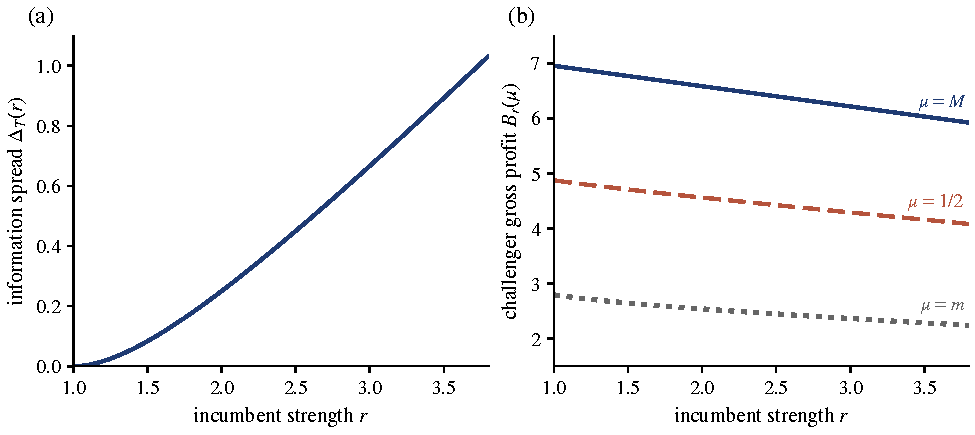
\includegraphics[width=\linewidth]{figures/two_returns.pdf}
\caption{Competition and the two returns to information.}\label{fig:1}
\par\medskip\begin{minipage}{\linewidth}\footnotesize\singlespacing\noindent \textit{Notes.} Panel (a) plots the target-payoff spread \(\Delta_T(r)\); panel (b)
plots gross challenger profit \(B_r(\mu)\) at the posterior bounds
\(m,M\) and the prior \(1/2\). Point-mass benchmark values are \(h=10\),
\(\ell=1\), \(p=0.5\), and \(b=2\). Values are per target share. These
are acquisition-stage payoffs, before solving trading and entry.\end{minipage}
\endgroup\end{figure}

Figure~\ref{fig:1} shows both effects within the benchmark support. The
target-payoff spread approaches zero as \(r\) approaches \(\ell\), since
the incumbent then almost never outbids a low-value challenger. As \(r\)
increases, the spread rises while gross acquisition profit falls at each
displayed belief. Whether entry rises depends on how this change in
payoffs affects equilibrium information.

\subsection{3.2 What the challenger learns from the
price}\label{sec-inference}

Noise demand bounds the posterior under every feasible trading strategy.
For arbitrary mixed orders, define

\[
\begin{aligned}
a_H(x)&=\int f(x-q)\,d\sigma_H(q),\qquad
&a_L(x)&=\int f(x-q)\,d\sigma_L(q),\\
\mu_X(x)&=\frac{\pi a_H(x)}{\pi a_H(x)+(1-\pi)a_L(x)},\qquad
&m(\pi)&=\frac{\pi}{\pi+(1-\pi)e^{2/b}},\quad
M(\pi)=\frac{\pi}{\pi+(1-\pi)e^{-2/b}}.
\end{aligned}
\tag{7}\label{eq:paper-7}
\]

The posterior satisfies \(m(\pi)\le\mu_X\le M(\pi)\). In the benchmark
\(\pi=1/2\), and I write \(m=m(1/2)=1/(1+e^{2/b})\) and
\(M=M(1/2)=1-m\). For any two orders \(q,q'\in[-1,1]\), the Laplace
density obeys

\[
e^{-2/b}\le\frac{f(x-q)}{f(x-q')}\le e^{2/b}.
\tag{8}\label{eq:paper-8}
\]

Integrating over the conditional order distributions preserves these
inequalities, so \(a_H/a_L\) lies in \([e^{-2/b},e^{2/b}]\). By Bayes'
rule the log odds of \(\mu_X\) are the log odds of \(\pi\) plus
\(\log(a_H/a_L)\), which gives the posterior bounds. Since the price is
a function of flow, the price-based posterior is a conditional
expectation of \(\mu_X\) and has the same bounds. A preparation decision
requiring a belief above \(M(\pi)\) cannot be induced by any equilibrium
price.

A zero-cost challenger pays nothing to prepare, and its expected gross
profit is never negative, so it prepares at every belief; the tie rule
covers a gross profit of zero. Averaging over preparation costs gives
the entry rule and candidate competitive price

\[
\begin{aligned}
e(\mu)&=\rho+(1-\rho)\mathbf1\{B(\mu)\ge c_H\},\\
P(\mu)&=t_0+e(\mu)[t_L-t_0+\Delta_T\mu].
\end{aligned}
\tag{9}\label{eq:paper-9}
\]

Under the restrictions of
\hyperref[sec-values-preparation-and-the-sale]{Section 2.2},
\(g_H\ge g_L\) and \(\Delta_T\ge0\) by \eqref{eq:paper-6}, and
\(t_L\ge t_0\). Both entry and the expected increment in target
proceeds therefore increase weakly with \(\mu\). When \(\Delta_T>0\) the
increment is strictly increasing, and entry is bounded below by
\(\rho>0\), so \(P(\mu)\) is strictly increasing. The price can jump
when high-cost preparation becomes worthwhile.

Price sufficiency holds in every candidate equilibrium in which the
classes differ in target proceeds, \(\Delta_T>0\). The entry floor
needs no condition. Let \(e(P)\) denote entry conditional on
the observed price, averaged over costs. Competitive pricing gives

\[
\begin{aligned}
P&=t_0+e(P)[t_L-t_0+\Delta_T\mu_X],\\
\mu_X&=\frac{P-t_0-e(P)(t_L-t_0)}{e(P)\Delta_T}.
\end{aligned}
\tag{10}\label{eq:paper-10}
\]

The denominator is at least \(\rho\Delta_T\), which is positive whenever
the classes differ in target proceeds. It makes \(\mu_X\) a measurable
function of \(P\). The challenger can therefore recover the market
maker's posterior from the price alone. This argument permits price
atoms and entry jumps. Propositions A.1 and A.2 give the formal
statements.

\subsection{3.3 Informed trading
incentives}\label{sec-informed-trading-incentives}

Rational pricing removes the anticipated increase in proceeds from the
investor's informational advantage. What remains depends on the
challenger's class. The residual advantages of buying in class \(H\) and
selling in class \(L\) are

\[
\begin{aligned}
A_H(x)&=\mathbb E[V_T\mid H,x]-P(x)=e(\mu_X(x))\Delta_T[1-\mu_X(x)],\\
A_L(x)&=P(x)-\mathbb E[V_T\mid L,x]=e(\mu_X(x))\Delta_T\mu_X(x),\\
\rho\kappa(\pi)\Delta_T&\le A_H(x),A_L(x)\le\Delta_T,\qquad
\kappa(\pi)=\min\{m(\pi),1-M(\pi)\}.
\end{aligned}
\tag{11}\label{eq:paper-11}
\]

The market maker prices the entry response. Noise demand still hides
the class. The investor's advantage is the entry probability times
the spread times the market's residual uncertainty. The lower bound
uses the entry floor \(\rho\) and \(1-\mu_X\ge1-M(\pi)\),
\(\mu_X\ge m(\pi)\). Since \(1-M(\pi)=m(1-\pi)\), \(\kappa(\pi)\)
equals \(m(\min\{\pi,1-\pi\})\). It equals \(m\) in the benchmark and
is smaller at every other prior. The class the prior favors binds,
because the price already leans toward it. The upper bound is
\(\Delta_T\). Both bounds hold under every candidate order
distribution. Their comparison with the trading cost sets when
information survives in equilibrium.

The no-entry proceeds \(t_0\) cancel from each residual in
\eqref{eq:paper-11}. Like the external dividend of
\hyperref[sec-access-to-prices]{Section 6.1}, \(t_0\) moves the price
and the terminal payoff together and leaves \(V_T-P\) unchanged. The
terms that matter are the entry gains \(t_H-t_0\) and \(t_L-t_0\).
Each gain is nonnegative, because an admissible challenger raises
proceeds to at least the reserve and an inadmissible one leaves them
unchanged. Both gains are strictly positive when no class value lies
at or below the reserve, as in the benchmark.

\section{4. Equilibrium results}\label{sec-results}

\subsection{4.1 Competition creates
competition}\label{sec-competition-creates-competition}

The main result identifies an open set of economies in which stronger
competition changes the unique trading and on-path preparation outcome
from an uninformative price with zero-cost preparation only to an
informative price with additional high-cost preparation.

\Needspace{8\baselineskip}

\protect\phantomsection\label{result-proposition-2}{\textbf{Proposition
2 (competition creates competition; analytical).}} \emph{Let the classes
satisfy the restrictions of
\hyperref[sec-values-preparation-and-the-sale]{Section 2.2}, so that the
high class dominates and both class supports lie above the reserve, let
\(F_1\)
be a continuous first-order stochastic strengthening of the continuous
incumbent distribution \(F_0\) (for uniform incumbents, \(r_0<r_1\)),
fix \(0<\pi<1\), \(0<\rho<1\), \(b>1\), and \(k>0\), and suppose that}

\[
B_{F_0}(\pi)<c_H<B_{F_1}(M(\pi)),
\tag{A1}\label{eq:paper-cond-1}
\]

\[
\Delta_T(F_0)<k<\left(1-\frac1b\right)\rho\,\kappa(\pi)\,\Delta_T(F_1).
\tag{A2}\label{eq:paper-cond-2}
\]

\emph{(i) With the weak incumbent \(F_0\), the unique equilibrium
trading outcome is \(q_H=q_L=0\), the price carries no information, and
entry equals \(\rho\). (ii) With the strong incumbent \(F_1\), the
unique equilibrium trading outcome is \((q_H,q_L)=(1,-1)\), the price is
informative, and entry strictly exceeds \(\rho\). Let
\(W_H(F)=\mathbb E_H[F(\theta)\mathbf1\{\theta\ge p\}]\) be the
probability that a prepared class-\(H\) challenger wins, and let
\(e_H\) be entry conditional on class \(H\) at \(F_1\). High-class
ownership, the probability that a class-\(H\) challenger acquires the
target, rises from \(F_0\) to \(F_1\) if and only if
\(e_HW_H(F_1)>\rho W_H(F_0)\). It rises whenever
\((1+\rho)W_H(F_1)\ge2\rho W_H(F_0)>0\), and so in the point-mass
benchmark, where \(W_H=1\). (iii) For any continuous first-order
stochastic strengthening \(F_2\) of \(F_1\) with
\(B_{F_2}(M(\pi))<c_H\), the unique trading outcome is again
\((1,-1)\), but entry returns to \(\rho\). For every pair of classes
with \(\mathbb E_H[\max\{\theta,p\}]>\mathbb E_L[\max\{\theta,p\}]\)
and every \(\pi\), \(\rho\), and \(b\), these conditions, the condition
of part (iii), and the sufficient ownership condition hold together on a
nonempty open set of uniform strengths \(r_0<r_1<r_2\) and costs
\((c_H,k)\). Uniqueness refers to trading and on-path entry under
truthful bidding and allows arbitrary mixed orders and every unilateral
deviation to an order in \([-1,1]\).}

Because the weak-incumbent price is uninformative and the strong-incumbent price is informative, the strong-incumbent price experiment strictly Blackwell-dominates the weak one at the same noise law (\citeproc{ref-Blackwell1953}{Blackwell 1953}).

A zero-cost challenger pays nothing and prepares after every price.
The floor does three jobs in the proofs. Entry stays at least
\(\rho\), so the denominator in \eqref{eq:paper-10} stays positive
and the price reveals the market's posterior. The residual advantage
stays at least \(\rho\kappa(\pi)\Delta_T\) at every flow
\eqref{eq:paper-11}, the bound that \eqref{eq:paper-cond-2} sets against
the trading cost. Zero-cost preparation does not respond to the price,
so information can only add entry. The floor \(\rho>0\) is therefore an
assumption with content: at \(\rho=0\), entry can vanish at unfavorable
prices, the price need not reveal the posterior, and the residual has no
positive lower bound. Gross profit is an expected auction rent and never
falls below zero. Any positive low cost below \(B_F(m(\pi))\) in every
economy in the comparison gives the same orders, prices, and entry,
because such a cost is covered at every feasible belief and the
low-cost challenger again prepares at every price.

Condition \eqref{eq:paper-cond-1} excludes high-cost preparation at the
weak-incumbent prior and permits it at favorable strong-incumbent
prices. Condition \eqref{eq:paper-cond-2} places the trading cost above
every informational return in the weak economy and below the global
bound on marginal trading profit in the strong economy. Its window is
nonempty exactly when
\(\Delta_T(F_0)/\Delta_T(F_1)<(1-1/b)\rho\kappa(\pi)\), a condition on
the two incumbent distributions, the classes, \(\rho\), \(b\), and
\(\pi\) that involves no unit of money. A prior away from one half
narrows the window, since \(\kappa(\pi)<m\) there.

The trading bound in \eqref{eq:paper-cond-2} is a worst case over every
candidate schedule and every mixture, so the proposition certifies a
corner of the region in which the reversal occurs.
\hyperref[sec-coexistence-and-the-equilibrium-correspondence]{Section
4.3} reports what lies between the two benchmark strengths. No trade is
the unique outcome below a sufficient bound and remains an equilibrium
up to an existence boundary. Three informative equilibria are certified
between these two bounds, and each coexists with no trade. Full orders
are unique above a second sufficient bound. None of these bounds locates
the first informative equilibrium.

The inequalities pin down trading before any order profile. In the
weak economy the gross advantage per unit is at most
\(\Delta_T(F_0)<k\). Every nonzero order loses money. The posterior
stays at the prior and only the zero-cost challenger prepares. In the
strong economy the residual lower bound pays for every increase in a
correctly signed order, on the whole interval and against mixed
candidates. Full correctly signed orders are necessary in every
equilibrium. \hyperref[paper-appendix]{Appendix A} derives the bound
and the price and entry schedules.

Under full orders, favorable prices cross the expensive challenger's
preparation threshold with positive probability. With \(g_H\) and
\(g_L\) evaluated at \(F_1\), define the threshold belief \(\tau\), its
corresponding flow \(x^*\), the class-conditional probabilities of
crossing it \(\alpha_H,\alpha_L\), class-conditional entry \(e_H,e_L\),
total entry \(\mathsf E\), and high-class ownership \(\mathsf O_H\) by

\[
\begin{aligned}
\tau&=\frac{c_H-g_L}{g_H-g_L},&
x^*&=\frac b2\left[\log\frac\tau{1-\tau}-\log\frac\pi{1-\pi}\right],\\
\alpha_H&=1-\frac12e^{(x^*-1)/b},&
\alpha_L&=\frac12e^{-(x^*+1)/b},\\
e_H&=\rho+(1-\rho)\alpha_H,&
e_L&=\rho+(1-\rho)\alpha_L,\\
\mathsf E&=\pi e_H+(1-\pi)e_L,&
\mathsf O_H&=\pi e_HW_H(F_1).
\end{aligned}
\tag{12}\label{eq:paper-12}
\]

The prior shifts the threshold flow by \(-(b/2)\log[\pi/(1-\pi)]\). In
the benchmark that shift is zero and \(W_H=1\), because \(h\) exceeds
the incumbent's support, so
\(\mathsf E=\rho+(1-\rho)(\alpha_H+\alpha_L)/2\) and
\(\mathsf O_H=[\rho+(1-\rho)\alpha_H]/2\).

Throughout, entry \(\mathsf E\) is the preparation probability, the
probability that the challenger pays its preparation cost. Under the
restrictions of
\hyperref[sec-values-preparation-and-the-sale]{Section 2.2} every
prepared challenger is an admissible bidder. The auction then has two
admissible bidders whenever the incumbent's value also meets the
reserve.
\hyperref[sec-design]{Section 6.3} separates preparation from sale and
from two admissible bidders when the reserve is raised. Condition
\eqref{eq:paper-cond-1} places \(\tau\) in \((\pi,M(\pi))\) and \(x^*\) in
\((0,1)\). Since \(\alpha_H>1/2>\alpha_L\), the additional entry is
tilted toward the high class.

Ownership needs its own condition when the class values overlap the
incumbent's support. A stronger incumbent then beats a prepared
class-\(H\) challenger more often, which lowers \(W_H\), so entry can
rise while high-class ownership falls. The condition in part (ii)
compares the two effects. It holds whenever the high class rarely loses
to the incumbent, and automatically when its values lie above the
incumbent's support in both economies.

At a sufficiently strong incumbent satisfying part (iii), even the
largest feasible belief fails to justify high-cost preparation. Trading
remains informative, but entry returns to \(\rho\). The proposition establishes a rise and a subsequent fall across the specified economies; \hyperref[sec-coexistence-and-the-equilibrium-correspondence]{Section 4.3} describes the strengths between them.

\subsection{4.2 Benchmark and information
controls}\label{sec-benchmark-and-information-controls}

The point-mass benchmark has prior \(1/2\), measures money in units of
the low value, \(\ell=1\), and uses incumbent strengths \(r_0=1.2\),
\(r_1=3\), and \(r_2=3.6\); \hyperref[pa-parameters]{Appendix A.8} lists
the full parameter vectors. The numbers in this section and in
\hyperref[sec-coexistence-and-the-equilibrium-correspondence]{Section 4.3}
refer to this benchmark. From \(r_0\) to \(r_1\), gross acquisition profit at
the prior falls from 4.804167 to 4.291667, while the target-payoff
spread rises from 0.016667 to 0.666667. Entry nevertheless rises from
0.250000 to 0.522757, and high-value challenger ownership rises from
0.125000 to 0.324192. At \(r_2\), entry returns to 0.250000.

At these strengths the spread ratio \(\Delta_T(r_0)/\Delta_T(r_1)\) is
0.025, below the bound \((1-1/b)\rho m\) of
0.034, so the trading-cost window of
\eqref{eq:paper-cond-2} is nonempty. The window is
\((0.0167,0.0224)\), and it
contains \(k=0.02\). It depends on the prior through
\(\kappa(\pi)\), and at the benchmark strengths it is nonempty only for
priors in \((0.404610,0.595390)\).
With the other benchmark inputs fixed, the hypotheses of parts (i) and
(ii) of \hyperref[result-proposition-2]{Proposition 2} hold for priors in
\((0.467850,0.538096)\). The
hypotheses of all three parts hold for priors in
\((0.467850,0.500424)\).
Away from these priors the costs or strengths must change;
\hyperref[sec-acquisition-values]{Section 5.2} reports such vectors at
priors 0.3 and
0.7.

\setcounter{table}{0}
\begin{table}[tbp]\begingroup\singlespacing\small\centering
\caption{Acquisition-stage payoffs in the benchmark.}\label{tab:1}
\begin{threeparttable}
\setlength{\tabcolsep}{3pt}
\begin{tabular*}{\linewidth}{@{\extracolsep{\fill}}p{0.58\linewidth}rr@{}}
\toprule
 & Weak ($r=1.2$) & Strong ($r=3$) \\
\midrule
Proceeds without a challenger, $t_0$ & 0.291667 & 0.416667 \\
Proceeds with a high-value challenger, $t_H$ & 0.704167 & 1.541667 \\
Proceeds with a low-value challenger, $t_L$ & 0.687500 & 0.875000 \\
Gross profit of a high-value challenger, $g_H$ & 9.295833 & 8.458333 \\
Gross profit of a low-value challenger, $g_L$ & 0.312500 & 0.125000 \\
Information spread, $\Delta_T = t_H - t_L$ & 0.016667 & 0.666667 \\
Expected gross profit at the prior, $B_r(1/2)$ & 4.804167 & 4.291667 \\
\bottomrule
\end{tabular*}
\begin{tablenotes}\footnotesize
\item Benchmark primitives $h=10$, $\ell=1$, $p=0.5$; values are incremental value per target share. $\Delta_T$ is the spread in expected target proceeds across challenger classes, not total merger value and not the trader's expected profit. Closed forms in the text agree with direct integration of the realized sale rule to within $10^{-9}$ (Online Appendix C.1).
\end{tablenotes}
\end{threeparttable}

\par\endgroup\end{table}

\setcounter{table}{1}
\begin{table}[tbp]\begingroup\singlespacing\small\centering
\caption{Equilibrium outcomes, information controls, and welfare.}\label{tab:2}
\begin{threeparttable}
\setlength{\tabcolsep}{3pt}
\begin{tabular*}{\linewidth}{@{\extracolsep{\fill}}p{0.325\linewidth}rrrrrll@{}}
\toprule
 & $q_H$ & $q_L$ & $\mathsf{E}$ & $\mathsf{O}_H$ & $\mathcal{R}_T$ & Evidence & Unique \\
\midrule
\multicolumn{8}{l}{\emph{Panel A. Equilibrium outcomes}} \\
Weak incumbent ($r=1.2$) & 0 & 0 & 0.250000 & 0.125000 & 0.392708 & analytical & yes \\
Strong incumbent ($r=3$) & 1 & -1 & 0.522757 & 0.324192 & 0.872392 & analytical & yes \\
Very strong incumbent ($r=3.6$) & 1 & -1 & 0.250000 & 0.125000 & 0.664236 & analytical & yes \\
\midrule
\multicolumn{8}{l}{\emph{Panel B. Information controls}} \\
Frozen informative orders, $r=1.2$ & 1 & -1 & 0.562178 & 0.350606 & 0.520039 & numerical diagnostic & n/a \\
Frozen informative orders, $r=3$ & 1 & -1 & 0.522757 & 0.324192 & 0.872392 & numerical diagnostic & n/a \\
Price hidden, $r=1.2$ & 0 & 0 & 0.250000 & 0.125000 & 0.392708 & analytical & yes \\
Price hidden, $r=3$ & 1 & -1 & 0.250000 & 0.125000 & 0.614583 & analytical & yes \\
\bottomrule
\end{tabular*}
\par\medskip
\begin{tabular*}{\linewidth}{@{\extracolsep{\fill}}p{0.46\linewidth}rrr@{}}
\toprule
 & Price observed & Price hidden & Gain \\
\midrule
\multicolumn{4}{l}{\emph{Panel C. Access to prices at $r=3$}} \\
Target proceeds $\mathcal R_T$ & 0.872392 & 0.614583 & 0.257809 \\
Net acquisition surplus $\mathcal W$ & 2.632301 & 2.552083 & 0.080218 \\
\bottomrule
\end{tabular*}
\begin{tablenotes}\footnotesize
\item Benchmark primitives, Laplace noise, cost atoms. $\mathsf{E}$ is the preparation probability, $\mathsf{O}_H$ the probability that a high-value challenger acquires the target, $\mathcal{R}_T$ expected target proceeds. Evidence is the result status of the row (analytical, computer-assisted, or numerical diagnostic); Unique records separately whether the continuation is the unique one under the stated bound. Panel A rows are analytical outcomes of Proposition 2.
\item Panel B rows are information controls: control is an experiment role, not an evidence class. The frozen rows are a fixed-profile control that imposes full orders at both strengths and lets the challenger reoptimize; the profile is not an investor equilibrium at $r=1.2$ and coincides with the equilibrium profile at $r=3$ while its role remains that of a control, so its Unique field is not applicable. The price-hidden rows are the reoptimized equilibria of the economy in which the price is withheld from the challenger. The matched-dividend invariance diagnostic of Section 6.1 is reported in the online matched-price panel.
\item Panel C: $\mathcal{W}$ is allocation value net of paid preparation costs, not target revenue. The four strict margins of Proposition 2 at $(r_0,r_1)=(1.2,3)$ are $\zeta_{H0}$ = $1.20\times10^{0}$, $\zeta_{H1}$ = $2.17\times10^{-1}$, $\zeta_0$ = $3.33\times10^{-3}$, $\zeta_1$ = $2.41\times10^{-3}$. The recorded low-cost diagnostic is $\zeta_L$ = $2.37\times10^{0}$. It is gross profit at the lowest feasible belief, not a hypothesis of Proposition 2.
\end{tablenotes}
\end{threeparttable}

\par\endgroup\end{table}

Table~\ref{tab:1} reports the acquisition payoffs. Table~\ref{tab:2}
separates the analytical outcomes of
\hyperref[result-proposition-2]{Proposition 2} from fixed-profile
controls. Holding informative orders fixed restores deterrence: entry
falls from 0.562178 to 0.522757 as the incumbent strengthens. At every
belief and cost realization, a decline in gross acquisition profit can
only remove a preparation incentive.
\hyperref[result-proposition-a-3]{Proposition A.3} states this result
for any fixed information experiment. The frozen profile is a control: full orders are unprofitable in the weak economy, so the profile is an equilibrium only in the strong economy.

Hiding prices from the challenger holds entry at \(\rho=0.25\) at both strengths. The challenger uses its prior and prepares only at
zero cost. Together, these comparisons identify the source of the reversal:
incumbent strength changes the information generated by trading, and the
resulting entry response can exceed the direct deterrence effect.

\subsection{4.3 Coexistence and the equilibrium
correspondence}\label{sec-coexistence-and-the-equilibrium-correspondence}

In the point-mass benchmark, informative and uninformative equilibria
coexist at some intermediate strengths.
\hyperref[result-proposition-3]{Proposition 3} establishes three
equilibria with full purchases and partial sales that coexist with no
trade. \hyperref[result-proposition-2]{Proposition 2} compares
\(r_0=1.2\) with \(r_1=3\). The correspondence below shows what the
search finds between them; it does not identify the first informative
equilibrium.

\Needspace{8\baselineskip}

\protect\phantomsection\label{result-proposition-3}{\textbf{Proposition
3 (coexisting informative equilibria; computer-assisted).}} \emph{At the
point-mass benchmark parameters of \hyperref[pa-parameters]{Appendix
A.8}, there exist equilibria \((q_H,q_L)=(1,-v_i)\) at strengths
\(r_i\) whose certified enclosures are}

\[
\begin{array}{c@{\qquad}c@{\qquad}c}
r_i&v_i&\mathsf E_i\\[3pt]
1.55&[0.46031618,\,0.46031620]&[0.5450528898,\,0.5450528922]\\
1.60&[0.70747537,\,0.70747539]&[0.5487563062,\,0.5487563085]\\
1.65&[0.90333198,\,0.90333201]&[0.5513607988,\,0.5513608020]
\end{array}
\tag{13}\label{eq:paper-13}
\]

\emph{The entry intervals are strictly ordered upward. Each of the three
economies also admits no trade with entry \(\rho\).}

The proof uses interval arithmetic to enclose exact solutions. For the
low-value investor, global strict concavity reduces optimality to a
marginal-profit root. Opposite endpoint signs place a root inside each
reported interval. For the high-value investor, a uniform derivative
bound verifies that full purchases dominate every smaller order
throughout the root bracket. Wrong-signed orders are unprofitable. The
resulting entry enclosures are disjoint, which establishes the
cross-economy ordering. \hyperref[paper-appendix]{Appendix A} reports
the certificate margins; Online Appendix B supplies the complete method.

\setcounter{figure}{1}
\begin{figure}[tbp]\centering\begingroup\singlespacing
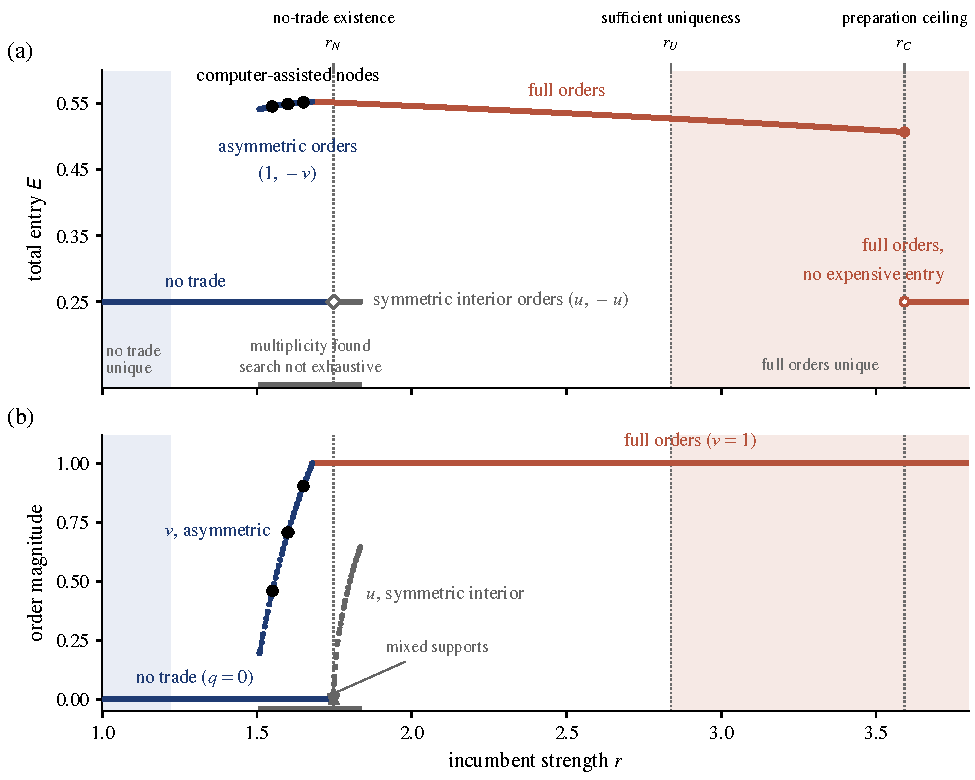
\includegraphics[width=\linewidth]{figures/equilibrium_correspondence.pdf}
\caption{Trading and entry across incumbent strengths.}\label{fig:2}
\par\medskip\begin{minipage}{\linewidth}\footnotesize\singlespacing\noindent \textit{Notes.} Benchmark parameters. Panel (a) shows preparation; panel (b) shows order
magnitudes. Shading marks analytical uniqueness regions; axis ticks mark strengths at which the search found several equilibria. \(r_N\) is the no-trade existence boundary, \(r_U\) the
sufficient full-order uniqueness bound, and \(r_C\) the high-cost
preparation ceiling. Black points carry the certified intervals of
\hyperref[result-proposition-3]{Proposition 3}. Other curves are numerical continuations; curves break where the search found no branch. A hollow diamond marks a
mixed candidate's preparation. Upward and downward triangles show its
support magnitudes after good and bad news, with size increasing in
probability weight. At \(r_C\), the filled circle includes preparation
at indifference, while the hollow circle marks the right-hand limit
after expensive preparation disappears. Online Appendix C.2 gives the methods.\end{minipage}
\endgroup\end{figure}

Figure~\ref{fig:2} places the certified equilibria within the numerical
correspondence. No trade remains an equilibrium up to
\(r_N=1.747877538\) and is uniquely optimal below the sufficient bound
\(\mathfrak r(k)=1.220997512\). Full orders are uniquely optimal above
the sufficient bound \(r_U=2.837416964\). High-cost entry becomes
infeasible above \(r_C=3.592658519\).
\hyperref[result-proposition-a-4]{Proposition A.4} defines these
thresholds. An existence boundary, a sufficient uniqueness bound, and a
participation ceiling answer different questions and need not coincide.

The numerical continuation finds asymmetric informative equilibria
before no trade disappears. On this family, the investor buys fully
after good news and sells partially after bad news. The short magnitude
increases toward one as the incumbent strengthens, and entry rises along
the accepted continuation. Full orders subsequently coexist with no
trade. The search also finds a symmetric interior family whose price
information is insufficient to induce high-cost preparation, so entry
remains \(\rho\). The finite-support search also retains a mixed
candidate at the no-trade existence boundary, shown as a numerical
diagnostic. 

The trading asymmetry reflects the entry response. Around the high-cost
preparation threshold, orders change both the posterior and the
probability of entry, and thus the residual payoff to information. The
low-value investor faces a different residual schedule from the
high-value investor and can stop at an interior short while full
purchases remain optimal. The certified points establish this behavior at three strengths.

No trade survives at the certified strengths because
\(\rho\Delta_T/2\le k\). Against an uninformative price with entry
\(\rho\), a unilateral informed order cannot cover its cost. An
informative equilibrium instead changes the preparation response and the
residual return to trading. The two outcomes can therefore be
self-consistent at the same parameters.

At \(r_C\), the Laplace posterior reaches its upper bound on a
positive-probability tail. The convention that an indifferent challenger
prepares preserves high-cost entry at the boundary itself; strictly
above it, that entry disappears. 

Outside the three certified points and the shaded analytical regions, the branches in Figure~\ref{fig:2} are numerical continuations from the search in Online Appendix C.2. That search also examined further pure and finite-support mixed profiles. The full correspondence at intermediate strengths is open.

\section{5. Robustness and private information}\label{sec-extensions}

\subsection{5.1 Noise and preparation
costs}\label{sec-noise-and-preparation-costs}

The reversal holds for the class of noise laws of
\hyperref[sec-trading-and-timing]{Section 2.3}. Let \(\mathcal N_L\)
denote the positive, absolutely continuous densities with
\(|(\log f)'|\le L\) almost everywhere, where \(0<L<1\), and set
\(b=1/L\). \hyperref[result-proposition-a-5]{Proposition A.5} extends the
equilibrium comparison to this class. Its upper cost restriction uses
the supremum of the posterior under full orders, which need not be
attained.

Laplace noise is the extreme member of the class. Among laws with median
zero, it has the thinnest tails at a fixed score bound. It gives the
most informative flow experiment at every pure order profile. The price
construction in Online Appendix A.6 preserves this comparison under its
stated conditions, and Online Appendix A.6 proves both claims.

Under full orders, the Laplace log odds relative to the prior odds equal
\((2/b)\max\{-1,\min\{x,1\}\}\). This is the Gaussian log odds with
variance \(b\), clipped at \(\pm2/b\). The linear part gives closed
forms, and the flat part keeps the market uncertain after extreme flows.
Gaussian noise has no finite score bound, and its posterior bounds do
not lie strictly inside \((0,1)\): an extreme flow all but reveals the
class, the residual advantage vanishes there, and the global argument
fails.

Logistic noise belongs to the class. At a common scale \(b\), logistic
noise equals Laplace noise plus independent noise. Under the same price
construction, the Laplace price experiment therefore Blackwell-dominates
the logistic experiment at the same orders. The logistic posterior
approaches its bounds only as flow tends to infinity.

In the strong benchmark economy, entry is 0.301509 under logistic noise,
compared with 0.522757 under Laplace noise (Table~\ref{tab:3}, Panel A). The logistic flow threshold
is 5.424598398, or 1.495369 noise standard deviations from the center.
The same posterior bounds can thus support different participation
rates, and the probability of favorable information near the upper bound
matters as well. At the same score bound and with full orders held
fixed, entry is 0.376606 under hyperbolic-secant noise and 0.374995 under
Student \(t_3\) noise. These two values are fixed-profile numerical
diagnostics: Online Appendix C.9 computes them without an equilibrium
search under these laws. Both lie between the logistic and the Laplace
values.

\setcounter{figure}{2}
\begin{figure}[tbp]\centering\begingroup\singlespacing
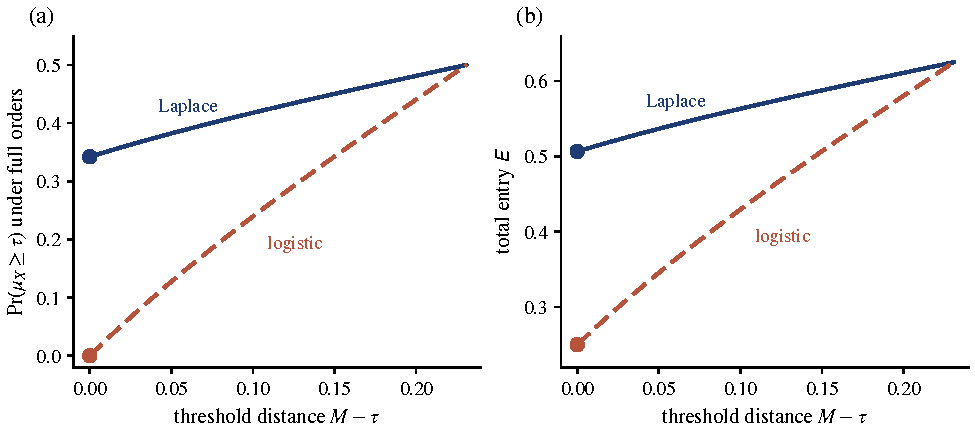
\includegraphics[width=\linewidth]{figures/posterior_tail_entry.pdf}
\caption{Posterior tails and high-cost entry.}\label{fig:3}
\par\medskip\begin{minipage}{\linewidth}\footnotesize\singlespacing\noindent \textit{Notes.} Full orders at the strong benchmark strength and scale \(b=2\). Panel
(a) plots \(\Pr(\mu_X\ge\tau)\) against \(M-\tau\); panel (b) plots
implied entry. At zero threshold distance, the Laplace plateau carries
positive mass and induces entry under the tie rule. The logistic tail
probability is zero there and is drawn as a closed point at zero mass in
panel (a) and at baseline preparation \(\rho\) in panel (b); the bound
is unattained by any posterior realization, but the plotted function is
defined at it. Common scale \(b\), not common variance, is held fixed
across the two noise laws. These are fixed-profile comparisons; Online Appendix C.5 checks the equilibrium at each implied cost.\end{minipage}
\endgroup\end{figure}

Figure~\ref{fig:3} compares the probability that the posterior exceeds
a preparation threshold near \(M\).
Laplace noise assigns positive probability to the upper posterior bound.
Logistic noise assigns none.
The comparison fixes a common scale and traces where posterior mass sits.
The Laplace experiment is more informative.
Informativeness does not order entry.

The result also holds when preparation costs are atomless.
The component with probability \(\rho\) starts at zero.
Its whole support lies below gross profit at the lowest feasible belief, so every
realization of it prepares at every feasible belief.
The other component lies above gross profit at the weak prior.
It lies below gross profit at the highest strong belief.
Its preparation therefore occurs only after sufficiently favorable prices in the strong
economy.
Entry then stays at or above \(\rho\), and the global trading bounds apply.
\hyperref[result-proposition-a-6]{Proposition A.6} states the result,
and \hyperref[paper-appendix]{Appendix A} gives the support
restrictions. With the declared atomless cost law, strong-incumbent entry
is 0.522715 under Laplace noise and 0.301374 under logistic noise.

\setcounter{table}{2}
\begin{table}[tbp]\begingroup\singlespacing\small\centering
\caption{Robustness and complementary private information.}\label{tab:3}
\begin{threeparttable}
\setlength{\tabcolsep}{3pt}
\begin{tabular*}{\linewidth}{@{\extracolsep{\fill}}p{0.26\linewidth}rrrrrll@{}}
\toprule
 & \shortstack{$\mathsf E$\\weak} & \shortstack{$\mathsf E$\\strong} & \shortstack{$\Delta\mathsf E$\\(pp)} & \shortstack{$\mathsf O_H$\\weak} & \shortstack{$\mathsf O_H$\\strong} & Evidence & Unique \\
\midrule
\multicolumn{8}{l}{\emph{Panel A. Noise and preparation costs}} \\
Laplace, cost atoms & 0.250000 & 0.522757 & 27.28 & 0.125000 & 0.324192 & analytical & yes \\
Laplace, cost mixture & 0.250000 & 0.522715 & 27.27 & 0.125000 & 0.324148 & analytical & yes \\
logistic, cost atoms & 0.250000 & 0.301509 & 5.15 & 0.125000 & 0.161994 & analytical & yes \\
logistic, cost mixture & 0.250000 & 0.301374 & 5.14 & 0.125000 & 0.161854 & analytical & yes \\
\midrule
\multicolumn{8}{l}{\emph{Panel B. Moderate values ($h=2$, $\ell=1$)}} \\
Moderate values & 0.250000 & 0.526805 & 27.68 & 0.125000 & 0.327032 & analytical & yes \\
\midrule
\multicolumn{8}{l}{\emph{Panel C. Complementary private information}} \\
$a=0.70$, $d=0.75$ & 0.850000 & 0.879438 & 2.94 & 0.425000 & 0.448942 & analytical & yes \\
\bottomrule
\end{tabular*}
\begin{tablenotes}\footnotesize
\item $\mathsf E$ is the preparation probability and $\mathsf O_H$ the probability of high-value challenger ownership, both probabilities. $\Delta\mathsf E=100(\mathsf E_{\mathrm{strong}}-\mathsf E_{\mathrm{weak}})$ is the change in preparation in percentage points, computed from the same validated probabilities as the two preparation columns, not a percentage change.
\item Each row is a distinct parameter vector (Appendix A.8): Panel A uses the benchmark vector with strengths $(1.2,3)$; Panel B uses the moderate-value vector with $(1.05,1.5)$; Panel C uses the complementary-signal vector with $(1.1,2.3)$, investor accuracy $a$ and buyer accuracy $d$. Panels B and C are separate illustrations, not one joint calibration. The cost mixture uses half-width $\varepsilon_C=0.1$; noise laws share the scale $b$, not the variance.
\item Evidence is the result status of the comparison. Unique records whether the sufficient uniqueness conditions of the relevant proposition hold. For cost atoms, these are four strict sufficient conditions. The cost mixture also requires the low-support margin in Proposition A.6. The online margins table retains all five recorded quantities and their minimum; the online accuracy-grid table reports the complete accuracy grid.
\end{tablenotes}
\end{threeparttable}

\par\endgroup\end{table}

\subsection{5.2 Value classes}\label{sec-acquisition-values}

The reversal holds without point masses, at any prior, and for any
class gap above the reserve, however small. Take any class pair under
the restrictions of
\hyperref[sec-values-preparation-and-the-sale]{Section 2.2} that
differs above the reserve. Take any prior, noise scale, and zero-cost
probability. \hyperref[result-proposition-2]{Proposition 2} then
holds, with its ownership condition, on a nonempty open set of
incumbent strengths and costs. The construction puts both strengths
just above the lowest value where the classes start to differ above
the reserve. The spread vanishes near that value, so informed trading
against the weaker incumbent cannot cover its cost. The profit gap
there stays near the full class value gap. A high cost that only
favorable prices justify fits in that gap. In the point-mass case
that value is \(\ell\), so the reversal holds for every \(h>\ell\). With
\(h=2\) and \(\ell=1\), the moderate-value specification satisfies all
strict inequalities of \hyperref[result-proposition-2]{Proposition 2}.
Entry rises from 0.250000 to 0.526805.
\hyperref[paper-appendix]{Appendix A} provides the construction; Online
Appendix C.4 records the numerical examples. With more than two
classes the price still reveals the whole posterior over classes, and
the comparison extends to two groups of classes (Online Appendix A.13).

Dispersed values within each class give a nondegenerate example. Let
values be uniform with half-width \(\varepsilon_V=0.05\) around \(\ell\)
and \(h\), let the prior be one half, and let the investor observe only
the class. \hyperref[sec-design]{Section 6.3} uses the same classes. At
the reserve \(p=0.5\) both classes lie above the reserve. At both benchmark
strengths the low class lies inside the incumbent's support and the high
class lies above it, so

\[
\Delta_T(r)=\frac{(r-\ell)^2+\varepsilon_V^2/3}{2r}.
\]

Dispersion within the low class adds to the spread. The benchmark vector
satisfies every strict inequality of
\hyperref[result-proposition-2]{Proposition 2} for these classes, and
preparation rises from 0.250000 to 0.522760 (Table~\ref{tab:5}, Panel
B). The restriction to supports above the reserve matters. At a reserve
that excludes the low class, equal admissibility fails, a stronger
incumbent can narrow the spread, and \hyperref[sec-design]{Section 6.3}
reports deterrence at such a reserve.

Table~\ref{tab:oa-class-exhibit} reports four economies outside the
benchmark. Cases A, B, and C satisfy every hypothesis of
\hyperref[result-proposition-2]{Proposition 2}, including that of part
(iii), and its sufficient ownership condition. Cases A and B keep the
point masses and set the prior at 0.3 and
0.7, where the benchmark vector violates
these hypotheses and no trading cost satisfies \eqref{eq:paper-cond-2}
at the benchmark strengths
(\hyperref[sec-benchmark-and-information-controls]{Section 4.2}). Each
of the two cases therefore has its own high cost, trading cost, and weak
strength, and entry rises from 0.250000 to
0.464564 in A and to 0.571808 in B.

Case C sets the prior at 0.7 and draws
values uniformly from \([0.6,1.4]\) and
\([1,19]\), wide classes above the
reserve with means \(\ell\) and \(h\). Its high class can lose to the
strong incumbent, so the ownership condition has content: at \(r_1\),
\(W_H\) falls to 0.924383, and high-class ownership
still rises from 0.175000 to
0.411984. Case D puts point masses at the same means
and keeps the costs, prior, and strengths of C. C raises strong-economy
entry to 0.563404, and D stays at
0.250000. Dispersion within a class raises the
challenger's option value of preparation. Preparation reveals the value,
and the challenger profits only when it wins, so its gross profit is
convex in the value; a spread around the same mean raises gross profit
at every belief. In C a favorable price lifts that profit above the high
cost, and in D even the largest feasible posterior does not. The class
model thus produces a reversal that the point-mass model with the same
means, costs, prior, and strengths cannot produce. D fails the upper
bound in \eqref{eq:paper-cond-1} at the strong strength, so its outcome
is not a counterexample to \hyperref[result-proposition-2]{Proposition 2}.

\setcounter{table}{3}
\begin{table}[tbp]\begingroup\singlespacing\small\centering
\caption{Quality classes and general priors.}\label{tab:oa-class-exhibit}
\begin{threeparttable}
\setlength{\tabcolsep}{3pt}
\begin{tabular*}{\linewidth}{@{\extracolsep{\fill}}lrlrrrr@{}}
\toprule
Case & $r$ & $(q_H,q_L)$ & $\mathsf E$ & $\mathsf O_H$ & $W_H$ & $x^*$ \\
\midrule
A & 1.1 & $(0,0)$ & 0.250000 & 0.075000 & 1.000000 & \textemdash \\
 & 3 & $(1,-1)$ & 0.464564 & 0.190421 & 1.000000 & 0.947381 \\
 & 3.6 & $(1,-1)$ & 0.250000 & 0.075000 & 1.000000 & none \\
\midrule
B & 1.1 & $(0,0)$ & 0.250000 & 0.175000 & 1.000000 & \textemdash \\
 & 3 & $(1,-1)$ & 0.571808 & 0.452851 & 1.000000 & 0.879481 \\
 & 3.6 & $(1,-1)$ & 0.250000 & 0.175000 & 1.000000 & none \\
\midrule
C & 1 & $(0,0)$ & 0.250000 & 0.175000 & 1.000000 & \textemdash \\
 & 4.5 & $(1,-1)$ & 0.563404 & 0.411984 & 0.924383 & 0.936639 \\
 & 5.5 & $(1,-1)$ & 0.250000 & 0.157102 & 0.897727 & none \\
\midrule
D & 1 & $(0,0)$ & 0.250000 & 0.175000 & 1.000000 & \textemdash \\
 & 4.5 & $(1,-1)$ & 0.250000 & 0.175000 & 1.000000 & none \\
 & 5.5 & $(1,-1)$ & 0.250000 & 0.175000 & 1.000000 & none \\
\bottomrule
\end{tabular*}
\par\medskip
\begin{tabular*}{\linewidth}{@{\extracolsep{\fill}}lrrrrrr@{}}
\toprule
Case & $c_H-B_0$ & $B_1(M)-c_H$ & $k-\Delta_0$ & $u_1-k$ & $c_H-B_2(M)$ & $s_W$ \\
\midrule
A & 1.460455 & 0.109179 & 0.005455 & 0.001349 & 0.058137 & 0.750000 \\
B & 0.562273 & 0.123413 & 0.005455 & 0.001349 & 0.132569 & 0.750000 \\
C & 0.021000 & 0.058891 & 0.006667 & 0.001770 & 0.314551 & 0.655478 \\
D & 0.025000 & -0.018122 & 0.020000 & 0.003171 & 0.447727 & 0.750000 \\
\bottomrule
\end{tabular*}
\begin{tablenotes}\footnotesize
\item All cases use $(h,\ell,p,\rho,b)=(10,1,0.5,0.25,2)$, zero low cost, and Laplace noise. A: $(\pi,c_H,k)=(0.3,4.5,0.01)$ and $(r_0,r_1,r_2)=(1.1,3,3.6)$. B: $(\pi,c_H,k)=(0.7,7.2,0.01)$ and $(r_0,r_1,r_2)=(1.1,3,3.6)$. C: $(\pi,c_H,k)=(0.7,6.7,0.02)$ and $(r_0,r_1,r_2)=(1,4.5,5.5)$. D: $(\pi,c_H,k)=(0.7,6.7,0.02)$ and $(r_0,r_1,r_2)=(1,4.5,5.5)$.
\item A, B, and D have point masses at $\ell$ and $h$. C has $G_L=U[0.6,1.4]$ and $G_H=U[1,19]$; D has the same class means and all other inputs as C.
\item $\mathsf E$ is preparation; $\mathsf O_H=\pi e_HW_H$ is high-class ownership. All displayed outcomes are unique by analytical bounds. The dash denotes no trade; \emph{none} denotes an unattainable high-cost threshold.
\item The first four margins are (A1)--(A2). Here $B_i=B_{r_i}(\pi)$ unless its argument is shown, $\Delta_i=\Delta_T(r_i)$, $u_1=(1-1/b)\rho\kappa(\pi)\Delta_1$, and $s_W=(1+\rho)W_H(r_1)-2\rho W_H(r_0)$. A--C satisfy Proposition 2, part (iii), and its sufficient ownership condition. D fails the upper bound in (A1); its full orders induce no high-cost entry. All hypotheses and independent checks appear in Online Appendix C.10.
\end{tablenotes}
\end{threeparttable}
\par\endgroup\end{table}


\subsection{5.3 Complementary private
information}\label{sec-complementary-private-information}

The challenger can benefit from prices even when its own information is
more accurate than the investor's. A buyer may know its integration
technology, while investors following the target hold information about
its customers or product market. Diligence combines these sources. I
represent this possibility with conditionally independent binary
signals: the investor observes \(T\) with accuracy \(a\), and the
challenger observes \(Y\) with accuracy \(d\), where \(a,d\in(1/2,1)\).
The challenger observes its signal and the price before preparing; preparation still
reveals the exact acquisition value.

Private information makes entry class-dependent even conditional on the
price. A challenger from the high-value class is more likely to receive favorable
private information and therefore more likely to prepare. Competitive
pricing incorporates both conditional entry rates. The zero-cost
realization prepares at every price, after either private signal.
Entry therefore stays at or above \(\rho\) in each class, the
coefficient on public beliefs stays strictly positive, and the price still reveals the market's posterior. The challenger
combines that posterior with its own signal.
\hyperref[paper-appendix]{Appendix A} derives the posterior formulas,
class-dependent pricing, and trading bounds.

\hyperref[result-proposition-a-7]{Proposition A.7} gives sufficient
conditions for unique zero orders and entry \(\rho\) in the weak
economy, and unique full orders by investor signal with entry above
\(\rho\) in the strong economy. The conditions allow arbitrary mixed
signal-contingent orders, every unilateral deviation to an order in
\([-1,1]\), and a buyer signal more accurate than the investor's. The
displayed sufficient conditions use the point-mass benchmark and prior
\(\pi=1/2\).

The example has buyer accuracy 75\% and investor accuracy 70\%.
Entry rises from 0.850000 to 0.879438. A favorable private signal alone
does not justify high-cost preparation against the weak incumbent;
combined with a favorable price, it does against the strong incumbent.
Table~\ref{tab:3} reports this example with the other robustness checks.
The full accuracy grid, including economies outside the sufficient uniqueness region, appears in Online Appendix C.3.

\section{6. Welfare and sale terms}\label{sec-welfare}

\subsection{6.1 Access to prices}\label{sec-access-to-prices}

Access to prices improves acquisition outcomes at a fixed level of
competition. Hold the incumbent at \(r_1\) and compare the feedback
equilibrium with an economy in which the challenger cannot observe the
price. All other parameters are unchanged, and trading and pricing are
reoptimized in both economies.
\hyperref[result-proposition-a-9]{Proposition A.9} establishes that
price access increases expected target proceeds and acquisition surplus
net of preparation costs. The comparison also holds with logistic noise
and with atomless preparation costs whose low component starts at zero.

The two economies generate the same order-flow experiment. The global
trading bound forces full orders even when the challenger cannot use the
price and entry remains \(\rho\). Trading costs therefore coincide.
Price access changes which high-cost challengers prepare. Each
additional preparation decision contributes at least the preparation
cost it incurs in conditional expectation, given the price information
and the cost realization that induce it; a challenger prepares only when
expected gross acquisition profit covers that cost. The allocation gain
includes that profit and the value of sales that would otherwise fail
the reserve. \hyperref[paper-appendix]{Appendix A} gives the accounting
identities. Transfers between bidders, shareholders, and traders are
excluded from acquisition surplus.

Table~\ref{tab:2} reports the fixed-strength comparison. Expected target
proceeds are 0.872392 with price access and 0.614583 without it.

Target shareholders gain because entry raises the value of their claim.
The gain is real, not a transfer. A shareholder who holds through the
sale receives \(V_T\), not the interim price. In the benchmark both
values lie above the reserve, so \(t_H>t_0\) and \(t_L>t_0\), and entry
raises expected proceeds in either class. At \(r_1\), price access
raises expected proceeds by 0.257809 per share. Under competitive
pricing the expected interim price rises by the same amount. The
informed investor's expected gross profit at one trading unit per share
of float is 0.140731. This profit is a transfer from liquidity traders:
the current shareholders who sell and the outside investors who buy.
Relative to an economy without the informed investor, initial
shareholders gain in total at every trade scale below 1.831923 trading
units per share of float, even if they bear the whole transfer. Online
Appendix C.9 computes both quantities. Holders who do not trade keep the
full proceeds gain. Holders who must sell bear part of the transfer and
can lose individually. The gain requires the recruiting region of
\hyperref[result-proposition-2]{Proposition 2}, in which high-cost
preparation does not pay at the prior. If high-cost preparation already
pays at the prior but not at the lowest feasible belief, an informative
price deters some preparation and lowers expected proceeds;
\hyperref[result-proposition-a-9]{Proposition A.9} states both cases.

The information effect can be separated from the average price level by
an analytical invariance diagnostic. Add a deterministic external
dividend of 0.257809 to the traded claim in the price-hidden economy.
The dividend raises both the terminal financial payoff and its price by
the same amount, leaving \(V_T-P\), trading incentives, seller revenue,
acquisition surplus, and entry unchanged. The mean financial price then
matches that of the feedback economy, while entry still differs. What
separates the two economies is the information the price carries, not
its level. The dividend is a diagnostic on the financial claim. No bidder pays it, the seller cannot choose it, and acquisition surplus excludes it. The matched-price table in the Online Appendix reports it beside
the hidden and feedback rows.

\subsection{6.2 The payment rule}\label{sec-the-payment-rule}

The effect of competition on the target-payoff spread depends on the sale payment. To isolate this dependence, consider a verifiable-value
institution with zero reserve. After diligence, the highest-value buyer
acquires the target. A sale to the next-best buyer at its value is an
enforceable fallback, accepted at zero surplus. The seller and winner
divide the surplus above this fallback by Nash bargaining, with seller share \(\eta\). Bulow and Klemperer (\citeproc{ref-BulowKlemperer1996}{1996}) compare an auction with one more bidder against an optimally structured negotiation by the seller's expected revenue; here the comparison is by how competition moves the target-payoff spread.

Without a challenger, the seller receives \(\eta R\). For point-mass
challenger values \(\ell\) and \(h\), an incumbent distribution supported
on \([0,\bar r]\) with \(\ell<\bar r<h\), and \(0\le\eta<1\), the
transfer, challenger profit, and target-payoff spread are

\[
\begin{aligned}
T_\eta(R,\theta)&=(1-\eta)\min\{R,\theta\}+\eta\max\{R,\theta\},\\
g_{\theta,\eta}&=(1-\eta)\mathbb E[(\theta-R)_+],\\
\Delta_\eta&=\eta(h-\ell)+(1-2\eta)\mathbb E[(R-\ell)_+].
\end{aligned}
\tag{14}\label{eq:paper-14}
\]

\hyperref[result-proposition-a-8]{Proposition A.8} establishes the
comparative statics. A stronger incumbent weakly reduces challenger
profit for every bargaining weight. Its effect on the target-payoff
spread is positive for \(\eta<1/2\), zero at \(\eta=1/2\), and negative
for \(\eta>1/2\), with strictness determined by the change in the
incumbent distribution.

To see why, take \(R>\ell\). A high-value challenger wins and pays
\((1-\eta)R+\eta h\), whose sensitivity to \(R\) is \(1-\eta\). A
low-value challenger loses, and the incumbent pays
\((1-\eta)\ell+\eta R\), whose sensitivity is \(\eta\). Competition
widens the difference precisely when the first sensitivity exceeds the
second. Thus the benchmark's opposition between acquisition profit and the target-payoff spread depends on the weight placed on the runner-up's value.

\setcounter{figure}{3}
\begin{figure}[tbp]\centering\begingroup\singlespacing
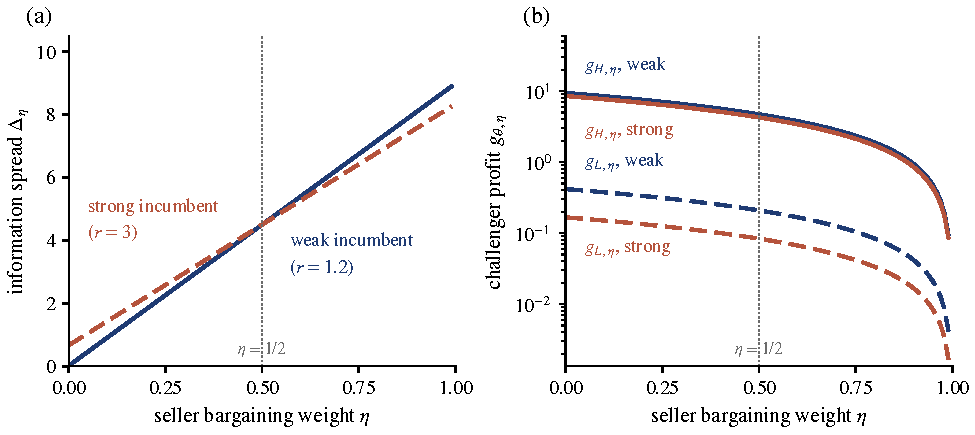
\includegraphics[width=\linewidth]{figures/bargaining_weight.pdf}
\caption{Bargaining and the division of acquisition surplus.}\label{fig:4}
\par\medskip\begin{minipage}{\linewidth}\footnotesize\singlespacing\noindent \textit{Notes.} Zero-reserve verifiable-value institution, \(h=10\), \(\ell=1\), and
uniform incumbents with \(r=1.2\) or \(r=3\). Panel (a) plots
\(\Delta_\eta\) against seller weight \(\eta\); panel (b) plots
conditional challenger profits on a log scale. Values are per target share. The log-scale panel uses seller weights below one.\end{minipage}
\endgroup\end{figure}

Figure~\ref{fig:4} illustrates these payment-stage results. Stronger competition weakly raises the target-payoff spread when the seller's weight is below one half, and strictly when it moves incumbent mass above \(\ell\). The trading and preparation game under bargaining is open.

\subsection{6.3 Reserve comparisons}\label{sec-design}

A reserve affects both the payment required to win and the information
embedded in target shares. A reserve that excludes the low-value class
can widen the difference in target proceeds across challenger classes. This can support informative trading even against a weak
incumbent. I illustrate this possibility with two reserve levels; the
seller's continuation problem and local revenue decomposition appear in
Appendix A.7.

Once the reserve can exclude bidders, preparation, sale, and competition
come apart. The preparation probability is the probability that the
challenger pays its preparation cost. The sale probability is the
probability that at least one bidder submits an admissible bid, whether
the incumbent or a prepared challenger whose realized value meets the
reserve. The probability of two admissible bidders is the probability
that both do. In the benchmark of \hyperref[sec-results]{Section 4} the
reserve lies below both challenger values, so every prepared challenger
is admissible. At a reserve above the low value, a prepared challenger
can learn that it cannot bid, and at a reserve above the incumbent's
support the incumbent is excluded. Preparation therefore measures acquisition competition only when both the prepared challenger and the incumbent are admissible. Table~\ref{tab:5} reports all
three probabilities beside expected target proceeds.

Use the value classes of
\hyperref[sec-acquisition-values]{Section 5.2}: uniform values with
half-width \(\varepsilon_V=0.05\) around \(\ell\) and \(h\), prior one
half, and an investor who observes only the class. Because the supports
have no atom, exclusion does not depend on an acquisition-value atom.
Increasing the reserve from 0.5 to
1.1 raises weak-incumbent expected proceeds from 0.392665 to 0.432173
and strong-incumbent expected proceeds from 0.872367 to 1.014500. At the
higher reserve, the preparation probability is 0.540309 and 0.511638,
respectively, and trading is informative in both economies. The global
bounds establish unique trading continuations at the reported reserve
choices.

\setcounter{table}{4}
\begin{table}[tbp]\begingroup\singlespacing\small\centering
\caption{Reserve comparisons.}\label{tab:5}
\begin{threeparttable}
\setlength{\tabcolsep}{3pt}
\begin{tabular*}{\linewidth}{@{\extracolsep{\fill}}p{0.28\linewidth}rrrrl@{}}
\toprule
Economy and reserve & Preparation & Sale & \shortstack{Two admissible\\bidders} & \shortstack{Expected target\\proceeds} & Trading outcome \\
\midrule
\multicolumn{6}{l}{\emph{Panel A. Binary values}} \\
Weak ($r=1.2$), $p=0.5$ & 0.250000 & 0.687500 & 0.145833 & 0.392708 & no trade \\
Weak ($r=1.2$), $p=1.01$ & 0.543573 & 0.443232 & 0.053595 & 0.452756 & full orders \\
Strong ($r=3$), $p=0.5$ & 0.522757 & 0.920460 & 0.435631 & 0.872392 & full orders \\
Strong ($r=3$), $p=1.01$ & 0.513373 & 0.770226 & 0.210611 & 0.987487 & full orders \\
\midrule
\multicolumn{6}{l}{\emph{Panel B. Atomless values with class information ($\varepsilon_V=0.05$)}} \\
Weak ($r=1.2$), $p=0.5$ & 0.250000 & 0.687500 & 0.145833 & 0.392665 & no trade \\
Weak ($r=1.2$), $p=1.1$ & 0.540309 & 0.391610 & 0.028025 & 0.432173 & full orders \\
Strong ($r=3$), $p=0.5$ & 0.522760 & 0.920460 & 0.435634 & 0.872367 & full orders \\
Strong ($r=3$), $p=1.1$ & 0.511638 & 0.749292 & 0.200293 & 1.014500 & full orders \\
\bottomrule
\end{tabular*}
\begin{tablenotes}\footnotesize
\item Preparation is the probability that the challenger pays its preparation cost. Sale is the probability that at least one bidder submits an admissible bid, whether the incumbent or a prepared challenger whose realized value meets the reserve. Two admissible bidders is the probability that both do. Expected target proceeds are seller revenue per share. All are validated outcome measures of the listed continuation at the declared reserve.
\item Benchmark primitives, Laplace noise, cost atoms; Panel B draws values uniformly around $\ell$ and $h$ with half-width $\varepsilon_V=0.05$ and gives the investor class information only. Analytical support: at every listed node the trading outcome is the unique continuation under the global bound ($k-\Delta_T>0$ for no trade; the uniform derivative bound with the automatic zero-cost entry floor for full orders). Order magnitudes, margins, evidence status, uniqueness scope, and the complete parameter identity of each node are in the online reserve-details table. The exploratory reserve summary (highest revenue among continuations found) is the online exploratory table.
\end{tablenotes}
\end{threeparttable}

\par\endgroup\end{table}

Table~\ref{tab:5} reports the two reserves. The higher reserve excludes the low-value class. It leaves the restrictions of \hyperref[sec-values-preparation-and-the-sale]{Section 2.2}, so \hyperref[result-proposition-1]{Proposition 1}(b) no longer applies, and a stronger incumbent can narrow the spread. The higher reserve changes both acquisition incentives and the target-payoff spread, and it raises expected proceeds in both economies. The seller-optimal reserve solves problem \eqref{eq:paper-a-44} of \hyperref[pa-design]{Appendix A.7}, which remains open; the Online Appendix reports an exploratory summary over the reserve domain.

With a zero preparation cost, entry is at least \(\rho\) at every price, at every reserve in
the domain of Appendix A.7. Wherever the target-payoff spread is positive, fixed orders
therefore fix what the price reveals. Distinct order-flow posteriors give distinct prices.
Only flows with one common posterior, such as a posterior plateau, share a price.
A continuation still consists of the complete object in
\hyperref[pa-design]{Appendix A.7}, because different orders can support different
continuations at one reserve. Online Appendix A.11 records what remains of price atoms
under the zero cost.

\section{7. Empirical implications}\label{sec-program}

The model gives three predictions for publicly visible sale processes in which one bidder is prepared and a further buyer has not yet committed to diligence. The first and third compare processes that differ in the public strength of the prepared bidder, as in \hyperref[result-proposition-2]{Proposition 2}; the second compares buyers within one process by the target return that preceded their decision.

First, when the target's price precedes the further buyer's decision, a stronger prepared bidder can raise the probability that the buyer starts diligence, as in the move from \(r_0\) to \(r_1\) in \hyperref[result-proposition-2]{Proposition 2}. When the price does not reach the buyer before its decision, a stronger prepared bidder weakly lowers that probability (\hyperref[result-proposition-a-3]{Proposition A.3}; Table~\ref{tab:2}, price-hidden rows).

Second, when informed trading is active, a further buyer that prepares after a favorable target return wins more often than one that prepares after an unfavorable return. In the benchmark, a high-value buyer always outbids the incumbent, and a low-value buyer loses whenever the incumbent's value exceeds \(\ell\). The preparation cost is independent of value, so at each price the share of high-value buyers among those that prepare equals the price-implied posterior, which rises with the price.

Third, against a sufficiently strong prepared bidder, further preparation returns to its floor and stops responding to the target's price, while the price stays informative (\hyperref[result-proposition-2]{Proposition 2}(iii)).

The empirical counterpart of preparation is the start of substantive diligence or the submission of a proposal that requires costly preparation; public offers are a narrower outcome. Incumbent strength is measured from information public before that decision, and the price information must precede it. Target returns before a bid also partly reflect anticipation of that bid (\citeproc{ref-Schwert1996}{Schwert 1996}), so each test dates the price before the buyer's decision and separates learning from anticipation. Online Appendix D sets out the design of an institutional pilot that dates these decisions and the public information sets from disclosure records.
The trading counterpart in these tests is outside trade with a view
on the further buyer's fit, such as sector-specialist flow, not trade
on whether an offer arrives.

\section{8. Conclusion}\label{sec-conclusion}

The bidder pool in a takeover depends on the information available
before buyers commit to participation. A stronger incumbent can increase
the sensitivity of target proceeds to challenger quality, making
informed trading profitable and bringing a challenger into the auction.
This connects the division of acquisition surplus to the formation of
competition. Sale terms therefore affect participation through both the
buyer's expected payment and the information supplied by the stock
market.

The next theoretical step is to characterize the seller's choice of
terms with the full pricing-and-trading continuation correspondence
retained, including the continuations that differ through their orders at one reserve.
The reserve comparisons show why this choice matters. A related question is whether committing
before trading improves outcomes relative to revising terms after
observing prices. Solving alternative auction formats and endogenous
investor research would clarify the role of payment rules and
manipulation incentives (\citeproc{ref-GoldsteinGuembel2008}{Goldstein
and Guembel 2008}). On the empirical side, the test is whether further preparation in publicly visible sale processes responds to incumbent strength as \hyperref[sec-program]{Section 7} predicts.

\clearpage

\section{References}\label{references}

\protect\phantomsection\label{refs}
\begin{CSLReferences}{1}{1}
\bibitem[\citeproctext]{ref-AcharyaJohnson2010}
Acharya, Viral V., and Timothy C. Johnson. 2010. {``More Insiders, More
Insider Trading: Evidence from Private-Equity Buyouts.''}
\emph{Journal of Financial Economics} 98 (3): 500--523.
\url{https://doi.org/10.1016/j.jfineco.2010.08.002}.

\bibitem[\citeproctext]{ref-AugustinBrennerSubrahmanyam2019}
Augustin, Patrick, Menachem Brenner, and Marti G. Subrahmanyam. 2019.
{``Informed Options Trading Prior to Takeover Announcements: Insider
Trading?''} \emph{Management Science} 65 (12): 5697--5720.
\url{https://doi.org/10.1287/mnsc.2018.3122}.

\bibitem[\citeproctext]{ref-BackEtAl2018}
Back, Kerry, Pierre Collin-Dufresne, Vyacheslav Fos, Tao Li, and
Alexander Ljungqvist. 2018. {``Activism, Strategic Trading, and
Liquidity.''} \emph{Econometrica} 86 (4): 1431--63.
\url{https://doi.org/10.3982/ECTA14917}.

\bibitem[\citeproctext]{ref-BettonEtAl2014}
Betton, Sandra, B. Espen Eckbo, Rex Thompson, and Karin S. Thorburn.
2014. {``Merger Negotiations with Stock Market Feedback.''} \emph{The
Journal of Finance} 69 (4): 1705--45.
\url{https://doi.org/10.1111/jofi.12151}.

\bibitem[\citeproctext]{ref-Blackwell1953}
Blackwell, David. 1953. {``Equivalent Comparisons of Experiments.''} \emph{The Annals of Mathematical Statistics} 24 (2): 265--72. \url{https://doi.org/10.1214/aoms/1177729032}.

\bibitem[\citeproctext]{ref-BondEdmansGoldstein2012}
Bond, Philip, Alex Edmans, and Itay Goldstein. 2012. {``The Real Effects of Financial Markets.''} \emph{Annual Review of Financial Economics} 4: 339--60. \url{https://doi.org/10.1146/annurev-financial-110311-101826}.

\bibitem[\citeproctext]{ref-BooneMulherin2007}
Boone, Audra L., and J. Harold Mulherin. 2007. {``How Are Firms Sold?''}
\emph{The Journal of Finance} 62 (2): 847--75.
\url{https://doi.org/10.1111/j.1540-6261.2007.01225.x}.

\bibitem[\citeproctext]{ref-BulowHuangKlemperer1999}
Bulow, Jeremy, Ming Huang, and Paul Klemperer. 1999. {``Toeholds and
Takeovers.''} \emph{Journal of Political Economy} 107 (3): 427--54.
\url{https://doi.org/10.1086/250068}.

\bibitem[\citeproctext]{ref-BulowKlemperer1996}
Bulow, Jeremy, and Paul Klemperer. 1996. {``Auctions Versus Negotiations.''} \emph{American Economic Review} 86 (1): 180--94. \url{https://www.jstor.org/stable/2118262}.

\bibitem[\citeproctext]{ref-CarlinEtAl2026}
Carlin, Bruce I., Tingting Liu, Micah S. Officer, Agathe Pernoud, and
Danni Tu. 2026. \emph{Bidder Pools in Mergers and Acquisitions}. Working
Paper No. 34846. National Bureau of Economic Research.
\url{https://doi.org/10.3386/w34846}.

\bibitem[\citeproctext]{ref-Clark1973}
Clark, Peter K. 1973. {``A Subordinated Stochastic Process Model with
Finite Variance for Speculative Prices.''} \emph{Econometrica} 41 (1):
135--55. \url{https://doi.org/10.2307/1913889}.

\bibitem[\citeproctext]{ref-Cont2001}
Cont, Rama. 2001. {``Empirical Properties of Asset Returns: Stylized
Facts and Statistical Issues.''} \emph{Quantitative Finance} 1 (2):
223--36. \url{https://doi.org/10.1080/713665670}.

\bibitem[\citeproctext]{ref-CornelliLi2002}
Cornelli, Francesca, and David D. Li. 2002. {``Risk Arbitrage in
Takeovers.''} \emph{The Review of Financial Studies} 15 (3): 837--68.
\url{https://doi.org/10.1093/rfs/15.3.837}.

\bibitem[\citeproctext]{ref-DowGoldsteinGuembel2017}
Dow, James, Itay Goldstein, and Alexander Guembel. 2017. {``Incentives
for Information Production in Markets Where Prices Affect Real
Investment.''} \emph{Journal of the European Economic Association} 15
(4): 877--909. \url{https://doi.org/10.1093/jeea/jvw023}.

\bibitem[\citeproctext]{ref-Edmans2009}
Edmans, Alex. 2009. {``Blockholder Trading, Market Efficiency, and
Managerial Myopia.''} \emph{The Journal of Finance} 64 (6): 2481--2513.
\url{https://doi.org/10.1111/j.1540-6261.2009.01508.x}.

\bibitem[\citeproctext]{ref-EdmansGoldsteinJiang2012}
Edmans, Alex, Itay Goldstein, and Wei Jiang. 2012. {``The Real Effects
of Financial Markets: The Impact of Prices on Takeovers.''} \emph{The
Journal of Finance} 67 (3): 933--71.
\url{https://doi.org/10.1111/j.1540-6261.2012.01738.x}.

\bibitem[\citeproctext]{ref-EdmansGoldsteinJiang2015}
Edmans, Alex, Itay Goldstein, and Wei Jiang. 2015. {``Feedback Effects,
Asymmetric Trading, and the Limits to Arbitrage.''} \emph{American
Economic Review} 105 (12): 3766--97.
\url{https://doi.org/10.1257/aer.20141271}.

\bibitem[\citeproctext]{ref-Fishman1988}
Fishman, Michael J. 1988. {``A Theory of Preemptive Takeover Bidding.''}
\emph{The RAND Journal of Economics} 19 (1): 88--101.
\url{https://doi.org/10.2307/2555399}.

\bibitem[\citeproctext]{ref-FoucaultFresard2014}
Foucault, Thierry, and Laurent Fr\'esard. 2014. {``Learning from Peers' Stock Prices and Corporate Investment.''} \emph{Journal of Financial Economics} 111 (3): 554--77. \url{https://doi.org/10.1016/j.jfineco.2013.11.006}.

\bibitem[\citeproctext]{ref-GentryLi2014}
Gentry, Matthew, and Tong Li. 2014. {``Identification in Auctions with
Selective Entry.''} \emph{Econometrica} 82 (1): 315--44.
\url{https://doi.org/10.3982/ECTA10293}.

\bibitem[\citeproctext]{ref-GentryStroup2019}
Gentry, Matthew, and Caleb Stroup. 2019. {``Entry and Competition in
Takeover Auctions.''} \emph{Journal of Financial Economics} 132 (2):
298--324. \url{https://doi.org/10.1016/j.jfineco.2018.10.007}.

\bibitem[\citeproctext]{ref-GoldsteinGuembel2008}
Goldstein, Itay, and Alexander Guembel. 2008. {``Manipulation and the
Allocational Role of Prices.''} \emph{The Review of Economic Studies} 75
(1): 133--64. \url{https://doi.org/10.1111/j.1467-937X.2007.00467.x}.

\bibitem[\citeproctext]{ref-GorbenkoMalenko2014}
Gorbenko, Alexander S., and Andrey Malenko. 2014. {``Strategic and Financial Bidders in Takeover Auctions.''} \emph{The Journal of Finance} 69 (6): 2513--55. \url{https://doi.org/10.1111/jofi.12194}.

\bibitem[\citeproctext]{ref-GrossmanHart1980}
Grossman, Sanford J., and Oliver D. Hart. 1980. {``Takeover Bids, the
Free-Rider Problem, and the Theory of the Corporation.''} \emph{The Bell
Journal of Economics} 11 (1): 42--64.
\url{https://doi.org/10.2307/3003400}.

\bibitem[\citeproctext]{ref-HirshleiferPng1989}
Hirshleifer, David, and I. P. L. Png. 1989. {``Facilitation of Competing
Bids and the Price of a Takeover Target.''} \emph{The Review of
Financial Studies} 2 (4): 587--606.
\url{https://doi.org/10.1093/rfs/2.4.587}.

\bibitem[\citeproctext]{ref-Imprivata2016}
Imprivata, Inc. 2016. \emph{Definitive Merger Proxy Statement, Form
{DEFM14A}}. U.S. Securities and Exchange Commission.
\url{https://www.sec.gov/Archives/edgar/data/1328015/000119312516677939/d226798ddefm14a.htm}.

\bibitem[\citeproctext]{ref-KotzKozubowskiPodgorski2001}
Kotz, Samuel, Tomasz J. Kozubowski, and Krzysztof Podg\'orski. 2001.
\emph{The Laplace Distribution and Generalizations: A Revisit with
Applications to Communications, Economics, Engineering, and Finance}.
Birkh\"auser.
\url{https://doi.org/10.1007/978-1-4612-0173-1}.

\bibitem[\citeproctext]{ref-Krishna2010}
Krishna, Vijay. 2010. \emph{Auction Theory}. 2nd ed. Academic Press.
\url{https://doi.org/10.1016/C2009-0-22474-3}.

\bibitem[\citeproctext]{ref-Kyle1985}
Kyle, Albert S. 1985. {``Continuous Auctions and Insider Trading.''} \emph{Econometrica} 53 (6): 1315--35. \url{https://doi.org/10.2307/1913210}.

\bibitem[\citeproctext]{ref-KyleVila1991}
Kyle, Albert S., and Jean-Luc Vila. 1991. {``Noise Trading and
Takeovers.''} \emph{The RAND Journal of Economics} 22 (1): 54--71.
\url{https://doi.org/10.2307/2601007}.

\bibitem[\citeproctext]{ref-LevinSmith1994}
Levin, Dan, and James L. Smith. 1994. {``Equilibrium in Auctions with
Entry.''} \emph{American Economic Review} 84 (3): 585--99.
\url{https://www.jstor.org/stable/2118069}.

\bibitem[\citeproctext]{ref-LinMaYangZhu2025}
Lin, Tse-Chun, Xiaorong Ma, Liyan Yang, and Minxing Zhu. 2025.
\emph{Payment Methods and Market Feedback in Mergers and Acquisitions}.
Working Paper 2025/189. HKU Jockey Club Enterprise Sustainability Global
Research Institute. \url{https://doi.org/10.2139/ssrn.5789982}.

\bibitem[\citeproctext]{ref-LiuBernhardt2022}
Liu, Tingjun, and Dan Bernhardt. 2022. {``Simplifying Auction Designs
via Market Feedback.''} Working paper.
\url{https://warwick.ac.uk/fac/soc/economics/staff/mdbernhardt/market_feedback_2022res_final.pdf}.

\bibitem[\citeproctext]{ref-Luo2005}
Luo, Yuanzhi. 2005. {``Do Insiders Learn from Outsiders? Evidence from
Mergers and Acquisitions.''} \emph{The Journal of Finance} 60 (4):
1951--82. \url{https://doi.org/10.1111/j.1540-6261.2005.00784.x}.

\bibitem[\citeproctext]{ref-MarmerShneyerovXu2013}
Marmer, Vadim, Artyom Shneyerov, and Pai Xu. 2013. {``What Model for
Entry in First-Price Auctions? A Nonparametric Approach.''}
\emph{Journal of Econometrics} 176 (1): 46--58.
\url{https://doi.org/10.1016/j.jeconom.2013.04.005}.

\bibitem[\citeproctext]{ref-Maug1998}
Maug, Ernst. 1998. {``Large Shareholders as Monitors: Is There a
Trade-Off between Liquidity and Control?''} \emph{The Journal of
Finance} 53 (1): 65--98.
\url{https://doi.org/10.1111/0022-1082.35053}.

\bibitem[\citeproctext]{ref-McAfeeMcMillan1987}
McAfee, R. Preston, and John McMillan. 1987. {``Auctions with Entry.''} \emph{Economics Letters} 23 (4): 343--47. \url{https://doi.org/10.1016/0165-1765(87)90142-X}.

\bibitem[\citeproctext]{ref-Meulbroek1992}
Meulbroek, Lisa K. 1992. {``An Empirical Analysis of Illegal Insider
Trading.''} \emph{The Journal of Finance} 47 (5): 1661--99.
\url{https://doi.org/10.1111/j.1540-6261.1992.tb04679.x}.

\bibitem[\citeproctext]{ref-PernoudGleyze2026}
Pernoud, Agathe, and Simon Gleyze. 2026. {``How Competition Shapes
Information in Auctions.''} Working paper.
\url{https://agathepernoud.com/Pernoud_Gleyze_InfoCompetition.pdf}.

\bibitem[\citeproctext]{ref-Persico2000}
Persico, Nicola. 2000. {``Information Acquisition in Auctions.''}
\emph{Econometrica} 68 (1): 135--48.
\url{https://doi.org/10.1111/1468-0262.00096}.

\bibitem[\citeproctext]{ref-RobertsSweeting2013}
Roberts, James W., and Andrew Sweeting. 2013. {``When Should Sellers Use
Auctions?''} \emph{American Economic Review} 103 (5): 1830--61.
\url{https://doi.org/10.1257/aer.103.5.1830}.

\bibitem[\citeproctext]{ref-Samuelson1985}
Samuelson, William F. 1985. {``Competitive Bidding with Entry Costs.''} \emph{Economics Letters} 17 (1--2): 53--57. \url{https://doi.org/10.1016/0165-1765(85)90126-0}.

\bibitem[\citeproctext]{ref-Schwert1996}
Schwert, G. William. 1996. {``Markup Pricing in Mergers and Acquisitions.''} \emph{Journal of Financial Economics} 41 (2): 153--92. \url{https://doi.org/10.1016/0304-405X(95)00865-C}.

\bibitem[\citeproctext]{ref-SmithSorensen2000}
Smith, Lones, and Peter S{\o}rensen. 2000. {``Pathological Outcomes of
Observational Learning.''} \emph{Econometrica} 68 (2): 371--98.
\url{https://doi.org/10.1111/1468-0262.00113}.

\bibitem[\citeproctext]{ref-Vickrey1961}
Vickrey, William. 1961. {``Counterspeculation, Auctions, and
Competitive Sealed Tenders.''} \emph{The Journal of Finance} 16 (1):
8--37. \url{https://doi.org/10.1111/j.1540-6261.1961.tb02789.x}.

\end{CSLReferences}

\clearpage

\section{Appendix A}\label{paper-appendix}

This appendix proves every result in the paper. Each statement
carries its status once: analytical, computer-assisted, numerical
diagnostic, or open. Statements use the class model of
\hyperref[sec-model]{Section 2}. A statement that needs the
point-mass benchmark says so. The Online Appendix holds the
probability-space construction, regular conditional distributions,
null-set invariance under deviations, convolution regularity, the
Stieltjes argument, interval endpoint ordering, the complete signal
laws, and the numerical definitions. Equations \eqref{eq:paper-1} to
\eqref{eq:paper-14} are in the main text.

\subsection{A.1 Acquisition payoffs and Bayesian
pricing}\label{pa-results}

\subsubsection{\texorpdfstring{Proof of
\hyperref[result-proposition-1]{Proposition
1}}{Proof of Proposition 1}}\label{proof-of-proposition-1}

Without entry the target receives \(p\mathbf1\{R\ge p\}\). A prepared
challenger with \(\theta\ge p\) wins at \(\theta>R\) and pays
\(\max\{p,R\}\). A loss makes the incumbent pay \(\theta\). The target
receives \(\max\{p,\min(R,\theta)\}\) and the challenger keeps
\((\theta-\max\{p,R\})_+\). At \(\theta<p\) the challenger does not
bid. The target again receives \(p\mathbf1\{R\ge p\}\) and the
challenger keeps nothing. Truthful bidding is weakly dominant at
every competing bid. No payoff here rests on a shading conjecture or
a belief. In the point-mass benchmark with the uniform incumbent,

\[
\begin{aligned}
t_H&=\frac1r\left[\int_0^p p\,du+\int_p^r u\,du\right],\\
t_L&=\frac1r\left[\int_0^p p\,du+\int_p^\ell u\,du+\int_\ell^r\ell\,du\right],\\
g_L&=\frac1r\left[\int_0^p(\ell-p)\,du+\int_p^\ell(\ell-u)\,du\right],
\end{aligned}
\tag{A.1}\label{eq:paper-a-1}
\]

which evaluate to \eqref{eq:paper-4} and differentiate to
\eqref{eq:paper-5}.

For general classes and a continuous \(F\), write the payments as
integrals of indicators. For \(\theta\ge p\),

\[
\max\{p,\min(R,\theta)\}=p+\int_p^\theta\mathbf1\{R>u\}\,du,
\qquad
(\theta-\max\{p,R\})_+=\int_p^\theta\mathbf1\{R<u\}\,du.
\tag{A.2}\label{eq:paper-a-2}
\]

The two indicators sum to one for almost every \(u\), which gives
\(t(\theta)+g(\theta)=\theta\). Tonelli's theorem applied to the
nonnegative integrands gives
\(t(\theta)=p+\int_p^\theta[1-F(u)]\,du\) and
\(g(\theta)=\int_p^\theta F(u)\,du\) for \(\theta\ge p\), while
\(t(\theta)=t_0=p[1-F(p)]\) and \(g(\theta)=0\) for \(\theta<p\). At
\(\theta=p\), \(t\) jumps by \(pF(p)\): when the incumbent fails the
reserve, an admissible challenger buys at \(p\) and an inadmissible one
leaves the target unsold. Hence, for every \(\theta\),

\[
t(\theta)=t_0+pF(p)\mathbf1\{\theta\ge p\}
+\int_p^\infty\mathbf1\{u\le\theta\}[1-F(u)]\,du,\qquad
g(\theta)=\int_p^\infty\mathbf1\{u\le\theta\}F(u)\,du .
\]

Take the class expectation and apply Tonelli's theorem again, with
\(\mathbb E_j\mathbf1\{\theta\ge p\}=1-G_j(p^-)\) and
\(\Pr_j(\theta\ge u)=1-G_j(u)\) for almost every \(u\). This gives

\[
t_j=t_0+pF(p)[1-G_j(p^-)]+\int_p^\infty[1-G_j(u)][1-F(u)]\,du
\]

and \(g_j\) in \eqref{eq:paper-6}; subtracting the classes gives
\(\Delta_T\) in \eqref{eq:paper-6}. The finite class means make every
integral finite. Since
\(\mathbb E_j[\max\{\theta,p\}]=p+\int_p^\infty[1-G_j(u)]\,du\), adding
the two lines of \eqref{eq:paper-6} gives the split in its general form,

\[
\Delta_T(F)+g_H(F)-g_L(F)
=pF(p)D(p^-)+\mathbb E_H[\max\{\theta,p\}]-\mathbb E_L[\max\{\theta,p\}].
\]

The reserve term vanishes under equal admissibility, and also when the
incumbent always meets the reserve, \(F(p)=0\).

\emph{Part (a).} In \eqref{eq:paper-6} the weight \(1-G_j\) on \(F\) is
nonnegative, so the pointwise decrease from \(F\) to \(\tilde F\) lowers
\(g_j\), strictly exactly when
\(\int_p^\infty[1-G_j][F-\tilde F]\,du>0\). Gross profit at a fixed
belief is an average of \(g_H\) and \(g_L\) with fixed weights, so it
falls as well.

\emph{Part (b).} Subtracting \eqref{eq:paper-6} at the two
distributions,

\[
\Delta_T(\tilde F)-\Delta_T(F)
=\int_p^\infty[F(u)-\tilde F(u)]D(u)\,du-p[F(p)-\tilde F(p)]D(p^-).
\]

Under the restrictions of
\hyperref[sec-values-preparation-and-the-sale]{Section 2.2} the second
term is zero and the integrand is nonnegative, so the spread rises,
strictly exactly when the integral is positive. Equal admissibility,
which also makes the second term zero, gives the same conclusion.

\protect\phantomsection\label{result-proposition-1c}{\textbf{Proposition
1(c) (the weakest restriction; analytical).}} \emph{For classes
\(G_H,G_L\) with finite means, the spread weakly increases under every
first-order stochastic strengthening of every continuous \(F\) if and
only if \(D(u)\ge0\) for every \(u>p\) and \(D(p^-)\le0\). When neither
class has an atom at \(p\), this condition is exactly first-order
dominance above the reserve together with equal admissibility,
\(G_H(p^-)=G_L(p^-)\).}

\emph{Proof of part (c).} Fix the incumbent's value \(R\). If \(R\ge p\), the
target receives \(\min\{R,\max\{\theta,p\}\}\) for every challenger
value: an admissible challenger and the incumbent both bid at least
\(p\), and an inadmissible challenger leaves the incumbent to pay \(p\).
If \(R<p\), the target receives \(p\mathbf1\{\theta\ge p\}\). Since
\(\mathbb E_j[\min\{R,\max\{\theta,p\}\}]=p+\int_p^R[1-G_j(u)]\,du\)
for \(R\ge p\), the expected difference in proceeds between the classes
at incumbent value \(R\) is

\[
\xi(R)=
\begin{cases}
pD(p^-), & R<p,\\[3pt]
\int_p^RD(u)\,du, & R\ge p,
\end{cases}
\]

and \(\Delta_T(F)=\mathbb E_F[\xi(R)]\). The function \(\xi\)
is bounded, constant below \(p\), continuous on \([p,\infty)\) with
derivative \(D\) almost everywhere, and moves from \(pD(p^-)\) to
\(\xi(p)=0\) at \(p\). It is nondecreasing if and only if
\(D\ge0\) almost everywhere above \(p\) and \(D(p^-)\le0\). If
\(\xi\) is nondecreasing, every first-order stochastic
strengthening raises \(\mathbb E_F[\xi(R)]\). If it is not,
continuity on each side of \(p\) gives points \(0<x_1<x_2\), both
different from \(p\), with \(\xi(x_1)>\xi(x_2)\). Let \(F\) be
uniform on \([x_1-\delta,x_1+\delta]\) and let \(\tilde F\) be the same law
shifted to \(x_2\). Then \(\tilde F\le F\), and as \(\delta\to0\),
\(\Delta_T(\tilde F)-\Delta_T(F)\to\xi(x_2)-\xi(x_1)<0\). If
the support must start at zero, mix the same small uniform component on
\([0,\bar r]\) into both laws; both mixtures are continuous, and the
mixing scales the difference by a positive factor and keeps its sign. Because distribution functions are
right-continuous, \(D\ge0\) almost everywhere above \(p\) is the same
as \(D(u)\ge0\) for every \(u>p\), and it implies \(D(p)\ge0\). When
neither class has an atom at \(p\), \(D(p^-)=D(p)\ge0\), so the
condition holds exactly when \(D(p^-)=0\), which with the ranking above
the reserve is equal admissibility.

Every result in the paper that assumes the restrictions of
\hyperref[sec-values-preparation-and-the-sale]{Section 2.2} also holds
when they are weakened to the ranking above the reserve and equal
admissibility. Its proof uses only \(D(u)\ge0\) for \(u>p\) and
\(D(p^-)=0\), which give \(g_H\ge g_L\) and \(\Delta_T\ge0\) in
\eqref{eq:paper-6}, the comparison in part (b), and the split identity of
\hyperref[sec-acquisition-profits-and-target-proceeds]{Section 3.1}.

For the point masses with \(p<\ell\), \(D(u)=\mathbf1\{\ell\le u<h\}\),
\(D(p^-)=0\), and \(\xi(R)=(R-\ell)_+\) for \(R<h\). Equation
\eqref{eq:paper-6} then gives \(\Delta_T=\int_\ell^h[1-F(u)]\,du\),
or \(\int_\ell^{\bar r}[1-F(u)]\,du\) at \(\bar r<h\), and
\(g_j=\int_p^\theta F(u)\,du\) at \(\theta=h\) and \(\theta=\ell\).
The kernel \(\xi\) belongs to the cash second-price rule with reserve.
\hyperref[sec-the-payment-rule]{Section 6.2} changes the rule and the
kernel with it. Online Appendix A.2 gives the measure formulation.
\(\square\)

\Needspace{10\baselineskip}

\subsubsection{Posterior bounds}\label{posterior-bounds}

\protect\phantomsection\label{result-proposition-a-1}{\textbf{Proposition
A.1 (posterior bounds; analytical).}} \emph{For arbitrary mixed
class-contingent orders on \([-1,1]\), the order-flow posterior
\(\mu_X\) and the posterior based on the price lie in
\([m(\pi),M(\pi)]\), where \(a_H\), \(a_L\), \(\mu_X\), \(m(\pi)\), and
\(M(\pi)\) are defined in \eqref{eq:paper-7}.}

For any feasible orders \(q,q'\) the triangle inequality gives
\(\big||x-q|-|x-q'|\big|\le|q-q'|\le2\), which is \eqref{eq:paper-8}.
Integrating against \(d\sigma_H(q)\,d\sigma_L(q')\) preserves both
inequalities, so \(e^{-2/b}a_L\le a_H\le e^{2/b}a_L\) for arbitrary
conditional mixtures. Since
\(\log[\mu_X/(1-\mu_X)]=\log[\pi/(1-\pi)]+\log(a_H/a_L)\), the log odds
of the posterior lie within \(2/b\) of the log odds of the prior, which
is \(m(\pi)\le\mu_X\le M(\pi)\). No monotone or pure strategy is
assumed. Because the price is a function of \(X\), the price posterior
is \(\mathbb E[\mu_X\mid P]\) by the tower property and inherits the
interval. The bounds satisfy \(1-M(\pi)=m(1-\pi)\), so
\(\kappa(\pi)=m(\min\{\pi,1-\pi\})\), and at \(\pi=1/2\) they are \(m\)
and \(M=1-m\). Online Appendix A.1 gives the measure-theoretic version,
including the null-set invariance under unilateral deviations.
\(\square\)

\Needspace{10\baselineskip}

\subsubsection{Price sufficiency and residual
profits}\label{price-sufficiency-and-residual-profits}

\protect\phantomsection\label{result-proposition-a-2}{\textbf{Proposition
A.2 (price sufficiency and residual profits; analytical).}}
\emph{Suppose \(\Delta_T>0\). In every candidate equilibrium the
observed price reveals \(\mu_X\) almost surely. Entry and competitive
pricing take the form \eqref{eq:paper-9}, and the residual advantages
of an informed buyer of shares in class \(H\) and of an informed short
seller in class \(L\) are given by \eqref{eq:paper-11}, with
\(\rho\kappa(\pi)\Delta_T\le A_H(x),A_L(x)\le\Delta_T\).}

\emph{Floor.} The zero-cost challenger pays nothing, and its gross profit
at every belief is an expectation of nonnegative auction rents, so it
prepares at every price, by the tie rule when that profit is zero.
Cost-averaged entry conditional on the price, \(e(P)\), is therefore at
least \(\rho\). This holds before any division and needs no condition on
beliefs.

\emph{Gross profit at a price.} The challenger's value depends on flow
only through its class, so its expected gross profit given the price is
\(\sum_j\Pr(j\mid P)g_j=B(\Pr(H\mid P))\). Its preparation decision
therefore depends on the price only through its posterior.

\emph{Inversion.} Entry depends on \((P,C)\), and \(C\) is independent
of the class and of flow, so
\(\mathbb E[V_T\mid j,x]=t_0+e(P(x))(t_j-t_0)\). Competitive pricing
gives the first line of \eqref{eq:paper-10} pointwise in flow, with
\(e(P)\) a function of the price. Since
\(e(P)\Delta_T\ge\rho\Delta_T>0\), the second line of
\eqref{eq:paper-10} expresses \(\mu_X\) as a Borel function of \(P\).
Conditioning \(\mu_X\) on the price therefore leaves it unchanged, and
\(\Pr(H\mid P)=\mathbb E[\mu_X\mid P]=\mu_X\) almost surely. Entry is
then \eqref{eq:paper-9} with the challenger's own posterior.

\emph{Construction.} Put \(w_L=t_L-t_0\ge0\). Under the restrictions of
\hyperref[sec-values-preparation-and-the-sale]{Section 2.2},
\(g_H\ge g_L\), so entry is nondecreasing in the belief. For
\(\mu_2>\mu_1\), \eqref{eq:paper-9} gives

\[
P(\mu_2)-P(\mu_1)
=e(\mu_2)\Delta_T(\mu_2-\mu_1)+[e(\mu_2)-e(\mu_1)](w_L+\Delta_T\mu_1)
\ge\rho\Delta_T(\mu_2-\mu_1)>0,
\tag{A.3}\label{eq:paper-a-3}
\]

because entry is nondecreasing and the bracket is nonnegative. The price
is therefore strictly increasing in the posterior, including across the
jump where high-cost preparation becomes worthwhile, and its inverse on
its image is measurable. A price value inside the skipped interval is
generated by no flow. A flat posterior tail maps into an actual price
atom, which is conditioned on as an atom.

\emph{Residuals.} Conditional on class \(j\) and flow \(x\), expected
terminal value is \(t_0+e(P(x))(t_j-t_0)\), in which the no-entry
proceeds and the public entry effect both appear. Subtracting the
rational price \(t_0+e(P(x))[w_L+\Delta_T\mu_X(x)]\) in class \(H\), and
reversing the subtraction in class \(L\), the terms \(t_0\) and
\(e\,w_L\) cancel and leave \eqref{eq:paper-11}. No unanticipated
premium is attached. This step uses neither the inversion nor the sign
of \(\Delta_T\). The bounds follow from \(\rho\le e\le1\) and
\(m(\pi)\le\mu_X\le M(\pi)\): \(A_H\ge\rho[1-M(\pi)]\Delta_T\) and
\(A_L\ge\rho m(\pi)\Delta_T\). If instead \(\Delta_T=0\), both residuals
vanish, every nonzero order loses its trading cost, and the posterior
stays at the prior, which the constant price then reveals. Online
Appendix A.3 supplies the conditional-probability argument. \(\square\)

\subsection{A.2 Global trading and the main comparison}\label{pa-proofs}

\subsubsection{The global order bound}\label{the-global-order-bound}

Fix a candidate pricing and preparation schedule. For a correctly signed
order of magnitude \(s\in[0,1]\) define

\[
\begin{aligned}
\bar A_H(s)&=\int f(x-s)A_H(x)\,dx,\qquad
\bar A_L(s)=\int f(x+s)A_L(x)\,dx,\\
U_j(s)&=s\bar A_j(s)-ks.
\end{aligned}
\tag{A.4}\label{eq:paper-a-4}
\]

The residual \(A_j\) is bounded and measurable but need not be
continuous, since it jumps where entry jumps. The deviation enters only
through the translated density. For \(s_1<s_2\),

\[
\bar A_j(s_2)-\bar A_j(s_1)
=\int_{s_1}^{s_2}\int \partial_u f(x\mp u)\,A_j(x)\,dx\,du,
\tag{A.5}\label{eq:paper-a-5}
\]

The Laplace density is absolutely continuous. Fubini's theorem
applies, because the absolute double integral is at most
\(\|A_j\|_\infty\,|s_2-s_1|\,\|f'\|_1\). So \(\bar A_j\) is absolutely
continuous, and \(|f'|\le f/b\) gives \(|\bar A_j'|\le \bar A_j/b\) almost
everywhere. A unilateral deviation never differentiates an entry jump.
The derivative falls on the density alone. With the residual lower
bound in \eqref{eq:paper-11},

\[
U_j'(s)=\bar A_j(s)+s\bar A_j'(s)-k
\ge\left(1-\frac sb\right)\bar A_j(s)-k
\ge\left(1-\frac1b\right)\rho\kappa(\pi)\Delta_T-k>0
\tag{A.6}\label{eq:paper-a-6}
\]

under the strong-incumbent inequality in \eqref{eq:paper-cond-2}, for every
\(s\in[0,1]\) and both classes. Integrating the positive lower bound
shows that the full correctly signed order strictly dominates every
smaller magnitude; this is global optimality, not a first-order
condition. The class-specific floors are \(\rho[1-M(\pi)]\Delta_T\) for
\(A_H\) and \(\rho m(\pi)\Delta_T\) for \(A_L\); \(\kappa(\pi)\) is the
smaller of the two. Online Appendix A.3 retains the \(W^{1,1}\) and
null-set details.

A sharper existence test applies to a fixed full-order candidate.
Substituting Bayes' rule with prior \(\pi\) into both residuals gives

\[
\begin{aligned}
\bar A_H(1)&=(1-\pi)K,\qquad \bar A_L(1)=\pi K,\\
K&=\Delta_T\int e(x)\frac{f(x-1)f(x+1)}{\pi f(x-1)+(1-\pi)f(x+1)}\,dx,
\end{aligned}
\tag{A.7}\label{eq:paper-a-7}
\]

so at \(\pi=1/2\) the two coincide, \(\bar A_H(1)=\bar A_L(1)=K/2\). The
pointwise ratio \(f(x-s)/f(x-1)\ge e^{-(1-s)/b}\) gives
\(\bar A_j(s)\ge e^{-(1-s)/b}\bar A_j(1)\). Since \((1-s/b)e^{-(1-s)/b}\) is
decreasing on \([0,1]\), the inequality
\(k<(1-1/b)\min\{\bar A_H(1),\bar A_L(1)\}\)
makes every correctly signed marginal profit positive against that
candidate. This verifies existence of the full-order profile; it says
nothing about other candidate schedules.

\subsubsection{\texorpdfstring{Proof of
\hyperref[result-proposition-2]{Proposition
2}}{Proof of Proposition 2}}\label{proof-of-proposition-2}

Steps 1 to 4 force the orders in every candidate equilibrium. Step 5
builds the price and preparation schedules at those orders.

\emph{Step 1: beliefs, the floor, and the payoff ranking.} Positivity of
\(f\) makes every conditional flow density positive, and
\hyperref[result-proposition-a-1]{Proposition A.1} gives
\(m(\pi)\le\mu_X\le M(\pi)\) under every trading strategy; the price
posterior obeys the same bound. The zero-cost challenger prepares at
every price in every economy, so cost-averaged entry is at least
\(\rho\) everywhere. Under the restrictions of
\hyperref[sec-values-preparation-and-the-sale]{Section 2.2},
\eqref{eq:paper-6} gives \(g_H\ge g_L\) and \(\Delta_T\ge0\) in each
economy. Condition \eqref{eq:paper-cond-2} with \(k>0\) gives
\(\Delta_T(F_1)>0\).
\hyperref[result-proposition-1]{Proposition 1}(a) gives
\(B_{F_1}(\pi)\le B_{F_0}(\pi)\), so \eqref{eq:paper-cond-1} gives
\(B_{F_1}(\pi)<c_H<B_{F_1}(M(\pi))\); since \(M(\pi)>\pi\), this forces
\(g_H(F_1)>g_L(F_1)\). The strengthening from \(F_0\) to \(F_1\) is
used here.

\emph{Step 2: residuals.} In either economy entry depends on the price
and the independent cost, and the challenger's value depends on flow
only through its class. Competitive pricing therefore gives
\(\mathbb E[V_T\mid j,x]=t_0+e(P(x))(t_j-t_0)\) and the residuals
\(A_H=e(P(x))\Delta_T(1-\mu_X)\) and \(A_L=e(P(x))\Delta_T\mu_X\), with
\(\rho\le e(P(x))\le1\), as in the residual step of
\hyperref[result-proposition-a-2]{Proposition A.2}. In the strong
economy, where \(\Delta_T(F_1)>0\), Proposition A.2 also gives
\(\Pr(H\mid P)=\mu_X\) almost surely and entry \eqref{eq:paper-9}. This
uses the independence of \(R\) and \(C\) from trading, not an assumption
that the challenger sees order flow.

\emph{Step 3: the weak economy.} A correctly signed order of size
\(s>0\) earns \(s[\bar A_j(s)-k]\le s[\Delta_T(F_0)-k]<0\) by the upper
bound \(A_j\le\Delta_T\) and the first inequality in
\eqref{eq:paper-cond-2}. A wrong-signed order has nonpositive gross payoff
and still pays its cost. Zero is therefore the only best response
against every candidate schedule, and a mixture placing positive
probability on nonzero orders averages strictly negative payoffs with
zero. Under zero orders \(X=Z\) and the posterior is \(\pi\);
\eqref{eq:paper-cond-1} gives \(B_{F_0}(\pi)<c_H\), so only the zero-cost
challenger prepares and entry is \(\rho\). The constant price
\(t_0+\rho[\pi t_H+(1-\pi)t_L-t_0]\) is competitive. This constructs the
unique outcome of part (i).

\emph{Step 4: the strong economy.} Against every candidate schedule,
\eqref{eq:paper-a-6} holds on the whole order interval. Every
equilibrium therefore has \((q_H,q_L)=(1,-1)\), and mixing cannot
introduce another optimal action.

\emph{Step 5: existence.} Full orders give

\[
\mu_X(x)=\left[1+\frac{1-\pi}{\pi}
\exp\left\{-\frac{|x+1|-|x-1|}{b}\right\}\right]^{-1},
\tag{A.8}\label{eq:paper-a-8}
\]

equal to \(m(\pi)\) on \(x\le-1\), strictly increasing on \((-1,1)\),
and equal to \(M(\pi)\) on \(x\ge1\). Define entry and price by
\eqref{eq:paper-9}. The strict monotonicity \eqref{eq:paper-a-3} gives a
measurable inverse on the price's image, including across its upward
jump and at the two plateau atoms. The challenger recovers the posterior from
the price, prepares optimally, and bids truthfully;
\eqref{eq:paper-a-6} verifies investor optimality; the price is
competitive by construction.

\emph{Step 6: comparisons.} By Step 1, \(\tau\in(\pi,M(\pi))\). On
\((-1,1)\) the log odds of \eqref{eq:paper-a-8} are
\(\log[\pi/(1-\pi)]+2x/b\), so high-cost preparation occurs exactly when
\(X\ge x^*\), with \(x^*\) in \eqref{eq:paper-12} and
\(x^*\in(0,1)\). Given class \(H\), \(X=1+Z\); given class \(L\),
\(X=-1+Z\). The Laplace survival function evaluated at \(x^*-1\) and
\(x^*+1\) gives \(\alpha_H\) and \(\alpha_L\) in \eqref{eq:paper-12},
both positive, so entry exceeds \(\rho\). Given its class and
preparation, the challenger's value is independent of the price, and it
wins with probability \(W_j(F)=\mathbb E_j[F(\theta)\mathbf1\{\theta\ge
p\}]\). High-class ownership is therefore \(\pi\rho W_H(F_0)\) at
\(F_0\) and \(\pi e_HW_H(F_1)\) at \(F_1\), which gives the stated
equivalence. Because \(x^*\in(0,1)\), \(\alpha_H>1/2\) and
\(e_H>(1+\rho)/2\), so \((1+\rho)W_H(F_1)\ge2\rho W_H(F_0)>0\) implies
\(e_HW_H(F_1)>\rho W_H(F_0)\). In the point-mass benchmark \(h\)
exceeds both incumbents' supports, so \(W_H=1\) in both economies and
\(\mathsf O_H=e_H/2>\rho/2\). Applying a constant kernel to the
strong-economy price reproduces the weak economy's constant experiment,
while no state-independent kernel applied to a constant experiment can
produce the nonconstant state-dependent price law of the strong economy;
the strong experiment therefore strictly Blackwell dominates the weak
one. All inequalities are strict and continuous in the primitives, so
for uniform incumbents the region is open in \((r_0,r_1,c_H,k)\);
\hyperref[pa-calculations]{Appendix A.4} shows that it is nonempty for
every pair of classes with
\(\mathbb E_H[\max\{\theta,p\}]>\mathbb E_L[\max\{\theta,p\}]\).

\emph{Part (iii).} Under the restrictions of
\hyperref[sec-values-preparation-and-the-sale]{Section 2.2},
\hyperref[result-proposition-1]{Proposition 1}(b) gives
\(\Delta_T(F_2)\ge\Delta_T(F_1)\), so the trading bound at \(F_2\)
follows from \eqref{eq:paper-cond-2}. The zero-cost floor and the derivative
bound give unique full orders exactly as in Steps 4 and 5, while
\(B_{F_2}(M(\pi))<c_H\) excludes every expensive entrant because
\(M(\pi)\) is the largest attainable belief under any strategy and
\(g_H(F_2)\ge g_L(F_2)\). Entry returns to \(\rho\). The condition on
\(F_2\) is separate from \eqref{eq:paper-cond-1} and \eqref{eq:paper-cond-2}
and establishes a rise and a subsequent fall across three economies, not
a monotone path. \(\square\)

\Needspace{10\baselineskip}

\subsubsection{Deterrence at a fixed
experiment}\label{deterrence-at-a-fixed-experiment}

\protect\phantomsection\label{result-proposition-a-3}{\textbf{Proposition
A.3 (deterrence at a fixed information experiment; analytical).}}
\emph{Let a signal \(S\) and the class have a fixed joint distribution,
let the challenger's value depend on \(S\) only through its class, and
let the preparation cost \(C\) be independent of the signal, the class,
and the value, with a fixed law, as in the model. Hold this experiment
and cost law fixed as the incumbent strengthens from \(F_0\) to a
first-order stochastic strengthening \(F_1\), so the challenger's posterior
\(\Pr(H\mid S)\) does not depend on the incumbent. Then entry is weakly
decreasing in incumbent strength. It decreases strictly when the decline
in gross profit crosses preparation costs on a positive-probability set
of signal and cost realizations.}

Write \(\mu(S)=\Pr(H\mid S)\); cost independence makes this the challenger's
complete posterior about the class, and its expected gross profit given
\(S\) is \(B(\mu(S))\) because its value depends on \(S\) only through
the class. By \hyperref[result-proposition-1]{Proposition 1}(a),
\(B_{F_1}(\mu)\le B_{F_0}(\mu)\) at every \(\mu\), for every pair of
classes, so

\[
\mathbf1\{C\le B_{F_0}(\mu(S))\}-\mathbf1\{C\le B_{F_1}(\mu(S))\}
=\mathbf1\{B_{F_1}(\mu(S))<C\le B_{F_0}(\mu(S))\}\ge0.
\tag{A.9}\label{eq:paper-a-9}
\]

Taking expectations proves the weak decrease and the exact strictness
condition, without an atomless cost distribution. The result applies
within a region of fixed full orders, where the conditional flow laws do
not depend on the incumbent; it does not apply across order profiles
that change with the incumbent, because changing orders change the
experiment. A version with cost correlated with the signal would
condition on \(\Pr(H\mid S,C)\) and is not needed here. \(\square\)

\Needspace{10\baselineskip}

\subsubsection{Threshold distinctions}\label{threshold-distinctions}

\protect\phantomsection\label{result-proposition-a-4}{\textbf{Proposition
A.4 (pooling, full orders, and expensive-entry feasibility;
analytical).}} \emph{In the point-mass benchmark, restrict attention to
the maintained domain
\(\mathcal D=\{r\in(\ell,h):B_r(1/2)<c_H\}\). Define}

\[
\begin{aligned}
\mathfrak r(d)&=\ell+d+\sqrt{d^2+2\ell d},\\
r_N&=\mathfrak r(2k/\rho),\qquad
r_U=\mathfrak r\left(\frac{k}{(1-1/b)\rho m}\right).
\end{aligned}
\tag{A.10}\label{eq:paper-a-10}
\]

\emph{No trade is an equilibrium exactly when
\(\rho\Delta_T(r)/2\le k\), that is, when \(r\le r_N\). The stronger
restriction \(r<\mathfrak r(k)\) guarantees that it is the unique
outcome. The restriction \(r>r_U\) guarantees unique full orders.
Expensive entry is impossible in every equilibrium when \(B_r(M)<c_H\).
If the equality \(B_r(M)=c_H\) has a solution in \(\mathcal D\), its
unique crossing is}

\[
r_C=\frac{Mh-c_H+\sqrt{(Mh-c_H)^2+M[(1-M)\ell^2-p^2]}}{M}.
\tag{A.11}\label{eq:paper-a-11}
\]

\emph{At \(r_C\) the tie rule of \hyperref[sec-model]{Section 2} is
retained.}

Under no trade the posterior is \(1/2\) and entry is \(\rho\), so a
unilateral correctly signed order of size \(s\) sees the constant
residual \(\rho\Delta_T/2\) and earns

\[
s\left(\frac{\rho\Delta_T(r)}{2}-k\right).
\tag{A.12}\label{eq:paper-a-12}
\]

Zero is optimal exactly when the coefficient is nonpositive. Solving
\(\Delta_T(r)=d\) gives \((r-\ell)^2=2rd\), whose root above \(\ell\) is
\(\mathfrak r(d)\); since \(\Delta_T\) is increasing, the
pooling-existence boundary is \(r_N\). Equality at \(r_N\) leaves the
investor indifferent among correctly signed sizes against that constant
schedule; it does not make every other profile an equilibrium with
recomputed prices. The sufficient uniqueness boundary \(\mathfrak r(k)\)
comes from \(\Delta_T<k\), which defeats any nonzero order against every
candidate schedule by Step 3 above. The full-order boundary \(r_U\)
comes from \eqref{eq:paper-a-6} at \(\pi=1/2\). The ceiling profit is

\[
B_r(M)=Mh-\frac{Mr}{2}+\frac{(1-M)\ell^2-p^2}{2r},
\tag{A.13}\label{eq:paper-a-13}
\]

strictly decreasing on \(r>\ell>p\), so it crosses \(c_H\) at most once;
\eqref{eq:paper-a-11} is the larger root of
\(Mr^2-2(Mh-c_H)r-[(1-M)\ell^2-p^2]=0\) and is the crossing when it lies
in \(\mathcal D\). Because \(M\) is the largest posterior under any
strategy, \(B_r(M)<c_H\) excludes expensive entry regardless of orders.
The four objects answer different questions: an existence boundary, two
sufficient uniqueness bounds, and a participation ceiling; none
identifies the first appearance of an informative equilibrium.

Equations \eqref{eq:paper-a-10}, \eqref{eq:paper-a-11}, and
\eqref{eq:paper-a-13} are point-mass formulas. The arguments extend.
With classes and prior \(\pi\), a unilateral order of size \(s\)
against the constant schedule at the prior earns
\(s[e(\pi)\Delta_T(1-\pi)-k]\) in class \(H\) and
\(s[e(\pi)\Delta_T\pi-k]\) in class \(L\), where \(e(\pi)\) is entry at
the prior. No trade is therefore an equilibrium exactly when
\(e(\pi)\Delta_T\max\{\pi,1-\pi\}\le k\), which is
\(\rho\Delta_T\max\{\pi,1-\pi\}\le k\) when \(B(\pi)<c_H\). The other
thresholds solve the same equations with \(\Delta_T\) and \(B\) from
\eqref{eq:paper-6}, \(M(\pi)\) in place of \(M\), and \(\kappa(\pi)\) in
place of \(m\).

Under full Laplace orders \(\mu_X=M\) on the positive-probability tail
\(x\ge1\), so indifference at \(r_C\) is not a null event and the tie
rule admits expensive entry on that tail. As \(r\uparrow r_C\), the
threshold \(x^*\to1\) and

\[
\alpha_H\to\frac12,\qquad\alpha_L\to\frac12e^{-2/b},\qquad
\mathsf E(r)\to\rho+\frac{1-\rho}{4}\left(1+e^{-2/b}\right),
\tag{A.14}\label{eq:paper-a-14}
\]

whereas strictly above \(r_C\) expensive entry is impossible. Under
logistic noise the posterior reaches \(M\) only in the limit, so
expensive entry converges to zero continuously
(\hyperref[pa-calculations]{Appendix A.4}). Online Appendix A.5 has the
domain checks. \(\square\)

\subsection{A.3 Certified asymmetric equilibria}\label{pa-certificate}

\subsubsection{Root definition}\label{root-definition}

Fix the point-mass benchmark primitives, with prior \(1/2\), and a strength \(r\). Candidate orders are
\((q_H,q_L)=(1,-v)\) with \(0<v<1\). Bayes' rule gives
\(\mu_v(x)=\operatorname{logistic}((|x+v|-|x-1|)/b)\), which ranges from
\(m_v=(1+e^{(1+v)/b})^{-1}\) to \(M_v=1-m_v\). In the certified region
\(1/2<\tau<M_v\), and

\[
\begin{aligned}
x^*(r,v)&=\frac{b\operatorname{logit}(\tau)+1-v}{2}\in(-v,1),\\
\mathsf E(r,v)&=\rho+\frac{1-\rho}{2}
\left[1-\frac12e^{(x^*-1)/b}+\frac12e^{-(x^*+v)/b}\right].
\end{aligned}
\tag{A.15}\label{eq:paper-a-15}
\]

The entry rule is \(e(x)=\rho+(1-\rho)\mathbf1\{x\ge x^*\}\) and the
residuals are \(A_H=e\Delta_T(1-\mu_v)\) and \(A_L=e\Delta_T\mu_v\). Let
\(\Psi(r,v)=U_L'(v;1,-v)\), where the derivative is taken in the
deviating magnitude \(s\) at \(s=v\) while the candidate schedule is
held fixed; recomputing the schedule as \(v\) varies is the outer
operation that makes \(\Psi\) a function of \(v\). The first is the
unilateral condition; the second changes the candidate.

\subsubsection{Low-type concavity}\label{low-type-concavity}

The unfavorable type's problem is globally concave. Its residual \(A_L\)
is bounded, nonconstant, and nondecreasing in \(x\), so it defines a
finite positive Stieltjes measure \(dA_L\), and integration by parts
gives

\[
\bar A_L'(s)=-\int f(x+s)\,dA_L(x)<0,
\qquad |\bar A_L''(s)|\le-\frac1b\bar A_L'(s)
\tag{A.16}\label{eq:paper-a-16}
\]

almost everywhere. The measure includes the entry jump as an atom, so no
derivative of that jump is omitted. Therefore
\(U_L''(s)=2\bar A_L'+s\bar A_L''\le(2-s/b)\bar A_L'(s)<0\) on \([0,1]\) whenever
\(b>1/2\), and \(U_L'\) is strictly decreasing. A root of the unilateral
marginal-profit equation is thus the unique global short magnitude
against its candidate schedule, including against the endpoints.

\subsubsection{Interval signs}\label{interval-signs}

Existence follows from an interval sign change. On a bracket
\([v_-,v_+]\) that keeps \(1/2<\tau<M_v\), the threshold \(x^*(r,v)\) is
continuous in \(v\), and dominated convergence makes \(\Psi(r,\cdot)\)
continuous. Outward interval evaluation proves that \(\Psi\) is positive
at the left endpoint of each bracket in
\hyperref[result-proposition-3]{Proposition 3} and negative at the right
endpoint, so the intermediate value theorem places an exact root inside.
Writing \(v_{i,-}\) and \(v_{i,+}\) for the endpoints of the bracket at
\(r_i\), the enclosures completing the sign tests are

\[
\begin{aligned}
\Psi(r_{\mathrm a},v_{\mathrm a,-})&\ge0.000000000114>0,&
\Psi(r_{\mathrm a},v_{\mathrm a,+})&\le-0.000000000096<0,\\
\Psi(r_{\mathrm b},v_{\mathrm b,-})&\ge0.000000000123>0,&
\Psi(r_{\mathrm b},v_{\mathrm b,+})&\le-0.000000000121<0,\\
\Psi(r_{\mathrm c},v_{\mathrm c,-})&\ge0.000000000172>0,&
\Psi(r_{\mathrm c},v_{\mathrm c,+})&\le-0.000000000242<0.
\end{aligned}
\tag{A.17}\label{eq:paper-a-17}
\]

Throughout each bracket the entry threshold stays strictly between
\(-v\) and \(1\). The sign change proves a root of \(\Psi(r,\cdot)\) on
the bracket, and the concavity result proves optimality at that root
against its own schedule; no uniqueness of the root across candidate
schedules is needed.

\subsubsection{High-type cover over the whole
bracket}\label{high-type-cover-over-the-whole-bracket}

A uniform derivative bound establishes optimality for the high-value
investor. For any bounded residual \(A_H\in[0,\Delta_T]\) the Laplace
kernel satisfies \(f''=(f-\delta_0)/b^2\) in the sense of distributions,
so

\[
\bar A_H''(s)=\frac{\bar A_H(s)-A_H(s)}{b^2}\quad\text{a.e.},\qquad
|U_H''(s)|\le L_U:=\frac{2\Delta_T}{b}+\frac{\Delta_T}{b^2}.
\tag{A.18}\label{eq:paper-a-18}
\]

On the mesh \(s_i=i/n\), interval arithmetic bounds \(U_H'(s_i)\)
uniformly over the whole root bracket \([v_-,v_+]\), not at a
floating-point midpoint. The exact root is known only to lie inside the
bracket, so the cover must hold for every candidate in it. Every
untested magnitude lies within \(1/(2n)\) of a mesh point, so

\[
\inf_{s\in[0,1]}U_H'(s)
\ge\min_i\underline{U_H'(s_i)}-\frac{L_U}{2n}>0.
\tag{A.19}\label{eq:paper-a-19}
\]

The certified global lower margins at the three strengths are
0.0000761777, 0.0027531948, and 0.0054921767. The favorable type
therefore chooses its maximum purchase, and all wrong-signed trades have
negative gross profit and are dominated by zero.

The integrals are elementary. Split each convolution at \(-v\), \(x^*\),
\(1\), and the deviation center. On the central region put \(c=(1-v)/2\)
and \(t=e^{(x-c)/b}\), so that \(\mu_v=t^2/(1+t^2)\). The primitives of
\(e^{x/b}(1-\mu_v)\), \(e^{-x/b}(1-\mu_v)\), \(e^{x/b}\mu_v\), and
\(e^{-x/b}\mu_v\) are respectively

\[
\begin{gathered}
b e^{c/b}\arctan t,\qquad
b e^{-c/b}(-t^{-1}-\arctan t),\\
b e^{c/b}(t-\arctan t),\qquad
b e^{-c/b}\arctan t.
\end{gathered}
\tag{A.20}\label{eq:paper-a-20}
\]

Constant-posterior tails integrate as exponentials without truncation.
Endpoint ordering is certified. When the low trader is evaluated at
\(s=v\) the center coincides with \(-v\) and is coalesced algebraically,
and distinct uncertain endpoints are ordered by disjoint interval
bounds. Online Appendix B has the full antiderivatives and the
endpoint-order rules.

\subsubsection{\texorpdfstring{No-trade coexistence and the proof of
\hyperref[result-proposition-3]{Proposition
3}}{No-trade coexistence and the proof of Proposition 3}}\label{no-trade-coexistence-and-the-proof-of-proposition-3}

No trade is also an equilibrium at each certified strength because
\(\rho\Delta_T(r_i)/2\le k\) there, by
\hyperref[result-proposition-a-4]{Proposition A.4}; the pooling margin
is enclosed with the same outward arithmetic. Interval arithmetic
applied to \eqref{eq:paper-a-20} encloses the root tests
\eqref{eq:paper-a-17}, the derivative cover \eqref{eq:paper-a-19}, the
pooling margin, and the entry probabilities \eqref{eq:paper-a-15}
throughout each bracket. The entry enclosures in \eqref{eq:paper-13} are
disjoint and ordered upward, which establishes the cross-economy
ordering. This is a computer-assisted existence proof in the sense of
Online Appendix B, with outward interval arithmetic on exact decimal
inputs. It does not prove uniqueness of the informative profile, exclude
mixed equilibria, or certify a continuous branch between the nodes.
\(\square\)

\subsection{A.4 Distributional extensions and
nonemptiness}\label{pa-calculations}

\subsubsection{Bounded-score noise}\label{logistic-noise}

Let \(\mathcal N_L\) denote the positive, absolutely continuous densities
\(f\) with \(|f'|\le Lf\) almost everywhere, where \(0<L<1\).
Equivalently, \(\log f\) is Lipschitz with constant \(L\).
Set \(b=1/L\).
The bounds \(m(\pi),M(\pi)\) and
\(\kappa(\pi)=\min\{m(\pi),1-M(\pi)\}\) use this value of \(b\).
For full orders, define

\[
\mu_f(x;\pi)=
\frac{\pi f(x-1)}{\pi f(x-1)+(1-\pi)f(x+1)},\qquad
\bar\mu_f(\pi)=\operatorname*{ess\,sup}_{x\in\mathbb R}\mu_f(x;\pi).
\]

The essential supremum uses Lebesgue measure.
The unconditional flow law and both conditional flow laws are equivalent to that measure.
The posterior is continuous, so this essential supremum equals \(\sup_{x\in\mathbb R}\mu_f(x;\pi)\).
The supremum satisfies \(\pi<\bar\mu_f(\pi)\le M(\pi)\).
It need not be attained at a finite flow.
It can lie strictly below \(M(\pi)\).

\Needspace{8\baselineskip}

\protect\phantomsection\label{result-proposition-a-5}{\textbf{Proposition
A.5 (bounded-score noise; analytical).}} \emph{Replace Laplace noise by
any \(f\in\mathcal N_L\).
Keep the quality-class assumptions of
\hyperref[result-proposition-2]{Proposition 2}, with preparation costs
\(C\in\{0,c_H\}\).
Replace the upper posterior in \eqref{eq:paper-cond-1} by \(\bar\mu_f(\pi)\), so that}

\[
B_{F_0}(\pi)<c_H<B_{F_1}(\bar\mu_f(\pi)).
\]

\emph{Retain \eqref{eq:paper-cond-2} with \(b=1/L\), namely}

\[
\Delta_T(F_0)<k<(1-L)\rho\kappa(\pi)\Delta_T(F_1).
\]

\emph{Then the weak economy has unique zero orders and entry \(\rho\).
The strong economy has unique full orders \((1,-1)\) and an informative price.
Let}

\[
\begin{aligned}
\tau&=\frac{c_H-g_L(F_1)}{g_H(F_1)-g_L(F_1)},
&\mathcal X_f&=\{x:\mu_f(x;\pi)\ge\tau\},\\
\alpha_H&=\int_{\mathcal X_f}f(x-1)\,dx,
&\alpha_L&=\int_{\mathcal X_f}f(x+1)\,dx.
\end{aligned}
\]

\emph{Total entry satisfies}

\[
\mathsf E_f=\rho+(1-\rho)[\pi\alpha_H+(1-\pi)\alpha_L]>\rho.
\]

\emph{High-class ownership rises exactly when
\([\rho+(1-\rho)\alpha_H]W_H(F_1)>\rho W_H(F_0)\).
The condition holds automatically in the point-mass case with \(W_H=1\).
Part (iii) of \hyperref[result-proposition-2]{Proposition 2} also holds at
a continuous first-order stochastic strengthening \(F_2\) of \(F_1\) with
\(B_{F_2}(M(\pi))<c_H\): orders remain \((1,-1)\), and entry equals \(\rho\).
For fixed \(f,L,\pi,\rho,p,G_H,G_L\) with
\(\mathbb E_H[\max\{\theta,p\}]>\mathbb E_L[\max\{\theta,p\}]\),
these comparisons and the ownership increase hold on a nonempty open set
of uniform strengths and costs \((r_0,r_1,r_2,c_H,k)\), with the zero
preparation cost fixed.}

\emph{Proof.}
The score bound gives
\(|\log f(y)-\log f(z)|\le L|y-z|\).
Hence \(f(y)\ge f(z)e^{-L|y-z|}\).
Integration over \(y\) gives \(f(z)\le L/2\).
Also \(\int|f'|\le L\), so \(f\in W^{1,1}\).
The density is positive, bounded, and continuous.
The null-set arguments in Online Appendix A.1 apply under every mixed order and every unilateral deviation.
\par
For any feasible \(q,q'\), the density ratio lies in \([e^{-2L},e^{2L}]\).
Integration over the order distributions and Bayes' rule give
\(m(\pi)\le\mu_X\le M(\pi)\).
Conditional expectation gives the same bounds for the price posterior.

The zero preparation cost gives \(e\ge\rho\) at every belief.
The price inversion and the residual calculation in Online Appendix A.3 apply without change.
They use only \(t_0,t_j,g_j,\Delta_T\), independence, and the positive entry floor.
In particular,

\[
\rho\kappa(\pi)\Delta_T\le A_H,A_L\le\Delta_T.
\]

The translation identity, Fubini argument, and product rule in Online Appendix A.3 allow this general \(f\).
They give \(|\bar A_j'|\le L\bar A_j\) and

\[
U_j'(s)\ge(1-sL)\bar A_j(s)-k
\ge(1-L)\rho\kappa(\pi)\Delta_T(F_1)-k>0.
\]

These steps differentiate the density.
They do not differentiate entry.
At \(F_0\), every correctly signed nonzero order earns at most
\(s[\Delta_T(F_0)-k]<0\).
A wrongly signed order loses as well.
Thus zero is the unique best response, including among mixed orders.
The posterior equals \(\pi\), and the lower cost restriction excludes expensive preparation.
The constant competitive price constructs the weak outcome.
\par
At \(F_1\), the positive derivative makes unit magnitude strictly optimal for each class.
It excludes every mixture with another order.
Define entry and price by \eqref{eq:paper-9}, with posterior \(\mu_f(x;\pi)\).
The price increases strictly in the posterior.
Its measurable inverse gives price sufficiency.
No monotonicity of the posterior in flow is required.
The construction gives competitive prices and optimal preparation.
The global bound verifies every order deviation.

Gross preparation profit falls with incumbent strength at every fixed belief.
The cost window therefore gives \(\pi<\tau<\bar\mu_f(\pi)\).
By the definition of the essential supremum, \(\{\mu_f>\tau\}\) has positive Lebesgue measure.
Both conditional densities are positive, so \(\alpha_H,\alpha_L>0\).
On \(\mathcal X_f\), Bayes' rule gives

\[
f(x-1)\ge
\frac{(1-\pi)\tau}{\pi(1-\tau)}f(x+1),\qquad
\alpha_H\ge\frac{(1-\pi)\tau}{\pi(1-\tau)}\alpha_L>\alpha_L.
\]

The entry formula and the stated ownership condition follow. The
likelihood ratio is not constant: both conditional densities integrate
to one, so a constant ratio would equal one, and \(f\) would be
two-periodic. No positive integrable density is two-periodic. The
nonconstant ratio therefore exceeds one on a set of positive measure,
so \(\bar\mu_f(\pi)>\pi\) and the strong price experiment is
informative. It strictly Blackwell-dominates the weak constant
experiment.
\par
For part (iii) of \hyperref[result-proposition-2]{Proposition 2},
\(\Delta_T(F_2)\ge\Delta_T(F_1)\) by \hyperref[result-proposition-1]{Proposition 1}(b), so the strict order
bound of \eqref{eq:paper-cond-2} holds at \(r_2\) with no separate condition.
It forces full orders, and \(\mu_X\le M(\pi)\) excludes expensive preparation.

For nonemptiness, fix \(f,L,\pi,\rho,p,G_H,G_L\) under the stated assumptions.
As in \hyperref[nonemptiness-for-every-value-gap]{the nonemptiness argument}, put

\[
\Gamma=\int_p^\infty[G_L(u)-G_H(u)]\,du>0,\qquad
u_0=\inf\left\{x\ge p:\int_p^x[G_L(u)-G_H(u)]\,du>0\right\}.
\]

For uniform incumbents, that argument gives \(\Delta_T(u_0)=0\) and \(g_H(u_0)-g_L(u_0)=\Gamma\).
The spread is continuous and strictly increasing above \(u_0\).
For finite \(r\ge u_0\), \(g_H(r)-g_L(r)\ge p\Gamma/r>0\).
The functions \(g_j(r)\) and \(W_H(r)\) are continuous and nonincreasing, with \(W_H(u_0)>0\).

\begin{enumerate}
\item
Choose \(\tau\in(\pi,\bar\mu_f(\pi))\) at a continuity point of the posterior law in each class.
Each law has at most countably many atoms, so such a point exists.
This fixes \(\mathcal X_f,\alpha_H,\alpha_L\) before any strength or cost is chosen.
In particular, \(\alpha_H,\alpha_L>0\).

\item
Choose \(r_1>u_0\) sufficiently near \(u_0\) that
\[
B_{r_1}(\tau)>B_{u_0}(\pi),\qquad
[\rho+(1-\rho)\alpha_H]W_H(r_1)>\rho W_H(u_0).
\]
The first inequality follows from
\(B_{u_0}(\tau)-B_{u_0}(\pi)=(\tau-\pi)\Gamma>0\).
The second follows from \(\alpha_H>0\) and \(W_H(u_0)>0\).
Continuity permits the same \(r_1\) in both inequalities.

\item
Set \(c_H=B_{r_1}(\tau)=g_L(r_1)+\tau[g_H(r_1)-g_L(r_1)]\).
Thus the preparation threshold equals the \(\tau\) chosen in the first step.
The positive profit gap gives \(c_H<B_{r_1}(\bar\mu_f(\pi))\).

\item
Choose \(r_0\in(u_0,r_1)\) sufficiently near \(u_0\) that
\[
\Delta_T(r_0)<(1-L)\rho\kappa(\pi)\Delta_T(r_1).
\]
This is possible because \(\Delta_T(r_0)\to0\) as \(r_0\downarrow u_0\).
Monotonicity gives \(B_{r_0}(\pi)\le B_{u_0}(\pi)<c_H\).
It also gives \(W_H(r_0)\le W_H(u_0)\), so the strict ownership inequality remains valid.

\item
Choose \(k\) strictly between \(\Delta_T(r_0)\) and
\((1-L)\rho\kappa(\pi)\Delta_T(r_1)\).
Both the preparation-cost window and the order-cost window now hold for this single choice of primitives.

\item
Choose \(r_2>r_1\) sufficiently large that \(B_{r_2}(M(\pi))<c_H\).
Finite class means give \(g_j(r)\to0\), so such a strength exists.
The larger spread preserves the strict order bound at \(r_2\).
\end{enumerate}

All inequalities have strict slack at the constructed point.
The threshold is continuous in \((r_1,c_H)\), since the class profit gap is positive.
At the chosen threshold, both conditional entry probabilities are continuous in that threshold.
The strict ownership inequality therefore persists on a neighborhood of \((r_0,r_1,r_2,c_H,k)\).
Continuity preserves the other strict inequalities there as well.
This proves openness in those five coordinates, with \(f,L,\pi,\rho,p,G_H,G_L\) and zero preparation cost fixed.
\(\square\)

\emph{Logistic example.}
The density

\[
f_{\mathrm{log}}(z)=\frac{1}{4b}\operatorname{sech}^{2}\left(\frac z{2b}\right)
=\frac{e^{-z/b}}{b(1+e^{-z/b})^2},\qquad b>1,
\tag{A.21}\label{eq:paper-a-21}
\]

has log derivative \(-\tanh(z/2b)/b\), so it belongs to \(\mathcal N_{1/b}\).
Under full orders its posterior satisfies

\[
\operatorname{logit}\mu_X
=\operatorname{logit}\pi
+2\log\cosh\left(\frac{x+1}{2b}\right)
-2\log\cosh\left(\frac{x-1}{2b}\right).
\tag{A.22}\label{eq:paper-a-22}
\]

The derivative is
\([\tanh((x+1)/2b)-\tanh((x-1)/2b)]/b>0\).
The posterior spans \((m(\pi),M(\pi))\) and attains neither endpoint.
Thus \(\bar\mu_f(\pi)=M(\pi)\).
The original upper restriction applies.
\par
Set \(A=e^{1/b}\) and
\(w=\sqrt{\tau(1-\pi)/[(1-\tau)\pi]}\).
With \(y=e^{x/b}\), the square root of the likelihood ratio is
\((Ay+1)/(y+A)\).
The equation \(w=(Ay+1)/(y+A)\) gives

\[
\begin{aligned}
x^*_{\mathrm{log}}&=b\log\frac{Aw-1}{A-w},\\
\alpha_H^{\mathrm{log}}&=\frac1{1+e^{(x^*_{\mathrm{log}}-1)/b}},\qquad
\alpha_L^{\mathrm{log}}=\frac1{1+e^{(x^*_{\mathrm{log}}+1)/b}}.
\end{aligned}
\tag{A.23}\label{eq:paper-a-23}
\]

These formulas hold for \(m(\pi)<\tau<M(\pi)\).
At \(\pi=1/2\), they reduce to the benchmark formulas.
The class also contains hyperbolic-secant noise, suitably scaled Student noise, and Gaussian noise plus an independent Laplace component.
Take these examples symmetric about zero, as are the Laplace and logistic laws above.
Each then satisfies the median-zero condition in Online Appendix A.6.

Laplace and logistic noise are compared at a common scale parameter \(b\).
At a common scale, the logistic law equals the Laplace law plus independent noise.
The Laplace flow experiment therefore Blackwell-dominates the logistic experiment at every order profile, pure or mixed
(\citeproc{ref-Blackwell1953}{Blackwell 1953}).
Under the price construction above, each price is a measurable function of flow and reveals its flow posterior.
Each price experiment is therefore Blackwell-equivalent to its flow experiment.
The same dominance holds for prices, including the full-order equilibria compared here.
Online Appendix A.6 proves the decomposition.
\par
At a common variance, neither experiment dominates in the numerical comparison.
That comparison is a numerical diagnostic.
Dominance does not order entry: \(\Pr(\mu_X\ge\tau)\) is not convex in the posterior.
The entry comparison turns on where posterior mass sits relative to the common bounds \(m(\pi),M(\pi)\).

\subsubsection{Atomless preparation
costs}\label{atomless-preparation-costs}

For atomless cost component distributions with
probabilities \(\rho\) and \(1-\rho\), supported within
\([0,2\varepsilon_C]\) and
\([c_H-\varepsilon_C,c_H+\varepsilon_C]\), the sufficient support
restrictions are

\[
\begin{gathered}
2\varepsilon_C<B_{F_1}(m(\pi)),\\
B_{F_0}(\pi)<c_H-\varepsilon_C<c_H+\varepsilon_C<B_{F_1}(M(\pi)),
\end{gathered}
\tag{A.24}\label{eq:paper-a-24}
\]

together with \eqref{eq:paper-cond-2}.

\Needspace{8\baselineskip}

\protect\phantomsection\label{result-proposition-a-6}{\textbf{Proposition
A.6 (atomless preparation costs; analytical).}} \emph{Retain the class
assumptions of \hyperref[result-proposition-2]{Proposition 2} and
condition \eqref{eq:paper-cond-2}, and replace the cost atoms by atomless
distributions satisfying \eqref{eq:paper-a-24}. Under either Laplace or
logistic noise, the unique trading outcomes and the entry reversal in
parts (i) and (ii) of Proposition 2 hold. High-class ownership rises
exactly when \(e_HW_H(F_1)>\rho W_H(F_0)\), where \(e_H\) is entry
conditional on class \(H\) at \(F_1\). This condition holds
automatically when \(W_H=1\) in both economies.}

Let \(H_C\) be the mixed cost CDF; the entry rule is
\(e(\mu)=H_C(B_F(\mu))\), continuous and nondecreasing. The first line
of \eqref{eq:paper-a-24} makes every realization of the component at
zero prepare at every feasible belief in both economies, since gross
profit at the lowest feasible belief \(m(\pi)\) already exceeds the
whole support and gross profit falls with incumbent strength. So
\(e\ge\rho\), and the residual bounds in \eqref{eq:paper-11} are
unchanged. The price increment \eqref{eq:paper-a-3} stays strictly
positive because \(H_C\) is nondecreasing, so the inversion and the
global trading bounds apply. At the weak prior, \(e(\pi)=\rho\) by both
lines of \eqref{eq:paper-a-24}. In the strong economy, beliefs close
enough to \(M(\pi)\) satisfy \(B_{F_1}(\mu)>c_H+\varepsilon_C\), an event
of positive probability under either noise law, and there \(e=1\).
Entry therefore exceeds \(\rho\). Given its class and preparation, the
challenger's value is independent of the price, so high-class ownership
is \(\pi\rho W_H(F_0)\) at \(F_0\) and \(\pi e_HW_H(F_1)\) at \(F_1\),
which gives the stated equivalence. Class-\(H\) flow reaches the event
above with positive probability, so \(e_H>\rho\), and \(W_H=1\) in both
economies gives the increase. The proof needs an atomless distribution,
not a density. Online Appendix A.6 has the details. \(\square\)

\subsubsection{Nonemptiness for every ranked pair of
classes}\label{nonemptiness-for-every-value-gap}

The region in \hyperref[result-proposition-2]{Proposition 2} needs no
large class gap and no special prior. Fix classes under
\hyperref[sec-values-preparation-and-the-sale]{Section 2.2}. Set
\(\Gamma(x)=\int_p^xD(u)\,du\). It is nondecreasing, with limit
\(\Gamma=\mathbb E_H[\max\{\theta,p\}]-\mathbb E_L[\max\{\theta,p\}]\).
Take classes that differ above the reserve, \(\Gamma>0\). Fix
\(\pi\in(0,1)\), \(b>1\), and \(\rho\in(0,1)\). Let
\(u_0=\inf\{x\ge p:\Gamma(x)>0\}\), the lowest value above which the
classes differ. In the point-mass benchmark \(u_0=\ell\) and
\(\Gamma=h-\ell\). Let \(F_r\) be the uniform distribution on \([0,r]\)
with \(r\ge p\). The kernel \(\xi\) in the proof of
\hyperref[result-proposition-1]{Proposition 1} equals \(\Gamma(R)\) for
\(R\ge p\) and, under the restrictions of
\hyperref[sec-values-preparation-and-the-sale]{Section 2.2} or more
generally under equal admissibility, zero for \(R<p\), so
\(\Delta_T(r)=r^{-1}\int_p^r\Gamma(u)\,du\). Hence \(\Delta_T(r)=0\) for
\(p\le r\le u_0\), and for \(r>u_0\) the spread is continuous and
strictly increasing, with derivative
\(r^{-2}[r\Gamma(r)-\int_p^r\Gamma(u)\,du]\ge p\Gamma(r)/r^2>0\). Since
\(\Gamma(x)\le\Gamma\), \(\Delta_T(r)\le(1-p/r)\Gamma\), and the split
in the proof of Proposition 1 gives
\(g_H-g_L=\Gamma-\Delta_T(r)\ge\Gamma p/r>0\). Dominated convergence,
with the finite class means, makes \(r\mapsto g_j(r)\) and
\(r\mapsto W_H(r)=\mathbb E_H[F_r(\theta)\mathbf1\{\theta\ge p\}]\)
continuous and gives \(g_j(r)\to0\) as \(r\to\infty\). Also
\(W_H(u_0)\ge(p/u_0)\Pr_H(\theta\ge p)>0\), because \(\Gamma>0\) gives
the high class mass above the reserve. At the limit \(r=u_0\),

\[
g_H-g_L=\Gamma,\qquad
B_{u_0}(M(\pi))-B_{u_0}(\pi)=[M(\pi)-\pi]\Gamma>0.
\tag{A.25}\label{eq:paper-a-25}
\]

Choose \(r_1>u_0\) close enough to \(u_0\) that
\(B_{r_1}(M(\pi))>B_{u_0}(\pi)\) and
\((1+\rho)W_H(r_1)>2\rho W_H(u_0)\). Since \(B_r(\pi)\) and \(W_H(r)\)
decrease in \(r\), every \(r_0\in(u_0,r_1)\) satisfies
\(B_{r_0}(\pi)<B_{r_1}(M(\pi))\) and
\((1+\rho)W_H(r_1)>2\rho W_H(r_0)>0\). Choose \(r_0\) close enough to
\(u_0\) that \(\Delta_T(r_0)<(1-1/b)\rho\kappa(\pi)\Delta_T(r_1)\),
which is possible because \(\Delta_T(r)\to0\) as \(r\downarrow u_0\).
Select \(k\) strictly inside the window of \eqref{eq:paper-cond-2} and
\(c_H\) strictly inside the window of \eqref{eq:paper-cond-1}; then
\(c_H>B_{r_0}(\pi)>0\). Since \(B_r(M(\pi))\to0\) as \(r\to\infty\),
some \(r_2>r_1\) has \(B_{r_2}(M(\pi))<c_H\), and
\(\Delta_T(r_2)\ge\Delta_T(r_1)\) gives the trading bound of part
(iii). All inequalities have strict slack and persist under small
perturbations of \((r_0,r_1,r_2,c_H,k)\) and of \((\pi,b,\rho)\), with
the low cost fixed at zero.

\subsection{A.5 Complementary private information}\label{pa-signals}

\subsubsection{Definitions}\label{definitions}

This subsection uses the point-mass benchmark with prior \(\pi=1/2\).
The investor observes a signal \(T\in\{+,-\}\) and the challenger a
signal \(Y\in\{+,-\}\), conditionally independent given quality, with
accuracies

\[
\begin{aligned}
\Pr(T=+\mid H)&=\Pr(T=-\mid L)=a,\\
\Pr(Y=+\mid H)&=\Pr(Y=-\mid L)=d,
\qquad a,d\in(1/2,1).
\end{aligned}
\tag{A.26}\label{eq:paper-a-26}
\]

Orders are contingent on \(T\): \(a_\pm(x)=\int f(x-q)\,d\sigma_\pm(q)\)
and \(\lambda_X=a_+/(a_++a_-)=\Pr(T=+\mid X)\). Public beliefs about
quality, their bounds, and the challenger's combined posteriors are

\[
\begin{aligned}
\mu_X&=(1-a)+(2a-1)\lambda_X,\\
\mu_-&=(1-a)+(2a-1)m,\qquad \mu_+=(1-a)+(2a-1)M,\\
\phi_+(\mu)&=\frac{d\mu}{d\mu+(1-d)(1-\mu)},\qquad
\phi_-(\mu)=\frac{(1-d)\mu}{(1-d)\mu+d(1-\mu)}.
\end{aligned}
\tag{A.27}\label{eq:paper-a-27}
\]

Set \(w_H=t_H-t_0\), \(w_L=t_L-t_0\), and
\(I_y=\mathbf1\{B_r(\phi_y(\mu))\ge c_H\}\) for \(y\in\{+,-\}\).
Class-conditioned entry rates and the price loading on public beliefs are

\[
\begin{aligned}
e_H&=\rho+(1-\rho)[dI_++(1-d)I_-],\\
e_L&=\rho+(1-\rho)[(1-d)I_++dI_-],\\
\Delta_P&=e_Hw_H-e_Lw_L.
\end{aligned}
\tag{A.28}\label{eq:paper-a-28}
\]

Entry is class-dependent even conditional on the price, so the
benchmark's common preparation rate is not reused here; the price
loading \(\Delta_P\) carries the two rates separately.

\Needspace{8\baselineskip}

\protect\phantomsection\label{result-proposition-a-7}{\textbf{Proposition
A.7 (complementary private signals; analytical).}} \emph{In the
point-mass complementary-signal economy with \(\pi=1/2\), choose
\(0<p<\ell<r_0<r_1<h\) and suppose}

\[
\begin{gathered}
B_{r_0}(d)<c_H<B_{r_1}(\phi_+(\mu_+)),\\
(2a-1)\{\Delta_T(r_0)+(1-\rho)(2d-1)w_H(r_0)\}<k
<\left(1-\frac1b\right)m(2a-1)\rho\Delta_T(r_1).
\end{gathered}
\tag{A.29}\label{eq:paper-a-29}
\]

\emph{The weak economy has unique zero informed orders and entry
\(\rho\). The strong economy has unique orders \(q(T=+)=1\) and
\(q(T=-)=-1\), and entry strictly exceeds \(\rho\). The conclusions
permit arbitrary mixed signal-contingent orders and every unilateral deviation to an order in \([-1,1]\), and do not require \(a\ge d\).}

\subsubsection{Proof}\label{proof}

Let \(J\in\{H,L\}\) denote the challenger's class.

\emph{Step 1: joint beliefs.} Flow depends on quality only through
\(T\), and \(Y\) is drawn from quality alone, so

\[
J\perp X\mid T,\qquad Y\perp X\mid J .
\tag{A.30}\label{eq:paper-a-30}
\]

The first relation gives \(\Pr(H\mid X)=a\lambda_X+(1-a)(1-\lambda_X)\),
which is the first line of \eqref{eq:paper-a-27}.
\hyperref[result-proposition-a-1]{Proposition A.1} applied to the
signal-contingent mixtures gives \(\lambda_X\in[m,M]\), hence
\(\mu_X\in[\mu_-,\mu_+]\), and the price posterior
\(\mu_P=\mathbb E[\mu_X\mid P]\) lies in the same interval. The second
relation survives any measurable function of \(X\), so Bayes' rule at
the price gives

\[
\Pr(H\mid P,Y=y)=\phi_y(\mu_P).
\tag{A.31}\label{eq:paper-a-31}
\]

Both maps \(\phi_y\) are continuous and strictly increasing, with
\(\phi_+>\phi_-\). The lowest joint posterior is \(\phi_-(\mu_-)\).
On this support gross profit is positive at every belief, so
\(B_{r_1}(\phi_-(\mu_-))>0\), and with \(B_{r_0}\ge B_{r_1}\) the
zero-cost realization prepares at every
reachable price in both economies under any candidate equilibrium, after either private signal.

\emph{Step 2: class-conditioned entry and price inversion.} Because the
law of \(Y\) given quality does not depend on \(X\), class-conditional entry
conditional on the price is \eqref{eq:paper-a-28} with \(I_y=I_y(P)\).
Since \(I_+\ge I_-\),

\[
e_H-e_L=(1-\rho)(2d-1)(I_+-I_-)\ge0,\qquad e_H\ge e_L\ge\rho,
\tag{A.32}\label{eq:paper-a-32}
\]

and, using \(w_H-w_L=\Delta_T\) and \(w_L>0\),

\[
\Delta_P=e_L\Delta_T+(e_H-e_L)w_H\ \in\ \big[\rho\Delta_T,\ \Delta_T+(1-\rho)(2d-1)w_H\big],
\qquad \Delta_P\ge\rho\Delta_T>0.
\tag{A.33}\label{eq:paper-a-33}
\]

Conditional competitive pricing is

\[
P=t_0+e_L(P)w_L+\mu_X\Delta_P(P),
\qquad
\mu_X=\frac{P-t_0-e_L(P)w_L}{\Delta_P(P)}.
\tag{A.34}\label{eq:paper-a-34}
\]

Both entry rates are functions of the price, so the positive loading
\(\Delta_P(P)\) makes \(\mu_X\) a Borel function of \(P\), the tower property
gives \(\mu_P=\mu_X\), and the affine map in \eqref{eq:paper-a-27} also
reveals \(\lambda_X\). For construction, write
\(P(\mu)=t_0+\mu e_H(\mu)w_H+(1-\mu)e_L(\mu)w_L\); for \(\mu_2>\mu_1\)
its increment is
\((\mu_2-\mu_1)\Delta_P(\mu_1)+\mu_2[e_H(\mu_2)-e_H(\mu_1)]w_H+(1-\mu_2)[e_L(\mu_2)-e_L(\mu_1)]w_L>0\),
so the price is strictly increasing even when both indicators jump at
once, and the measurable inverse of
\hyperref[result-proposition-a-2]{Proposition A.2} applies.

\emph{Step 3: residual bounds.} Conditional on \(T=+\) the investor
assigns quality probability \(a\), and conditional on \(T=-\) it assigns
\(1-a\); a unilateral order adds no quality information beyond the
signal. Its expected terminal payoff at flow \(x\) is
\(t_0+e_L(P(x))w_L+a\Delta_P(P(x))\) after \(T=+\), and the same expression
with \(1-a\) after \(T=-\). Subtracting \eqref{eq:paper-a-34} and using
\eqref{eq:paper-a-27},

\[
A_+=(2a-1)(1-\lambda_X)\Delta_P,\qquad A_-=(2a-1)\lambda_X\Delta_P,
\tag{A.35}\label{eq:paper-a-35}
\]

and \eqref{eq:paper-a-33} with \(\lambda_X\in[m,M]\) gives

\[
m(2a-1)\rho\Delta_T\le A_+,A_-
\le(2a-1)[\Delta_T+(1-\rho)(2d-1)w_H]=:A^+.
\tag{A.36}\label{eq:paper-a-36}
\]

\emph{Step 4: exclusion, global inequality, construction, and additional
entry.} In the weak economy the lower bound on \(k\) in
\eqref{eq:paper-a-29} makes any correctly signed order of magnitude
\(s>0\) earn at most \(s(A^+(r_0)-k)<0\); wrong signs have
negative gross payoff. Zero is therefore necessary under every candidate
schedule. With zero orders the public posterior is \(1/2\), the challenger's
favorable posterior is \(\phi_+(1/2)=d\), and \(B_{r_0}(d)<c_H\)
excludes expensive preparation after either private signal; entry is
\(\rho\) and constant pricing constructs the equilibrium. In the strong
economy the translation formula \eqref{eq:paper-a-5} applies to either
bounded residual, and the lower bound in \eqref{eq:paper-a-36} with the
upper bound on \(k\) in \eqref{eq:paper-a-29} gives

\[
U'(s)\ge\left(1-\frac1b\right)m(2a-1)\rho\Delta_T(r_1)-k>0
\tag{A.37}\label{eq:paper-a-37}
\]

on the whole order interval, so the unique trading profile is full
correctly signed orders by signal. Bayes' rule, the price in Step 2, and
optimal preparation using \eqref{eq:paper-a-31} construct the
equilibrium. Under full orders \(\lambda_X=M\) on the
positive-probability tail \(x\ge1\), where \(\mu_X=\mu_+\); the
condition \(c_H<B_{r_1}(\phi_+(\mu_+))\) then gives \(I_+=1\), and
\(\Pr(Y=+\mid J)>0\) in both classes. Additional preparation
therefore has positive probability and entry strictly exceeds \(\rho\).
Online Appendix A.7 gives the complete conditional laws and the
closed-form entry probabilities. \(\square\)

\subsection{A.6 Bargaining and access to prices}\label{pa-welfare}

\subsubsection{The verifiable-value
institution}\label{the-verifiable-value-institution}

The displayed bargaining formulas use point-mass challenger values
\(\ell\) and \(h\). The institution of
\hyperref[sec-the-payment-rule]{Section 6.2} has four elements: buyer values are verifiable after diligence; a sale to the
runner-up at its value is an enforceable fallback, accepted at zero
surplus; without a challenger the reserve is zero and the seller
bargains against a fallback of zero; and the seller's Nash bargaining
weight is \(\eta\).

\Needspace{8\baselineskip}

\protect\phantomsection\label{result-proposition-a-8}{\textbf{Proposition
A.8 (bargaining; analytical).}} \emph{In the verifiable-value
institution, let \(R\) have any distribution supported on
\([0,\bar r]\) with \(0<\ell<\bar r<h\). For \(0\le\eta<1\) the
institution generates \eqref{eq:paper-14}. A first-order stochastic
strengthening of the incumbent weakly reduces challenger profits. It
weakly increases the target's information spread for \(\eta<1/2\),
leaves that spread unchanged at \(\eta=1/2\), and weakly decreases it
for \(\eta>1/2\). Strictness follows from a positive integral change in
the corresponding payoff function.}

With fallback \(z\) and winning value \(V>z\), the transfer solves

\[
\max_{P\in[z,V]}(P-z)^\eta(V-P)^{1-\eta},
\tag{A.38}\label{eq:paper-a-38}
\]

whose log objective is strictly concave, giving
\(P=z+\eta(V-z)=(1-\eta)z+\eta V\); at \(V=z\) the feasible set is the
point \(z\), and at \(\eta=0\) I use the continuous limit \(z\). Without
a challenger the same rule with fallback zero pays the seller
\(\eta R\). The highest-value buyer receives the target and a challenger
wins only if \(\theta\ge R\), keeping \((1-\eta)(\theta-R)\), which
gives \(g_{\theta,\eta}\) in \eqref{eq:paper-14}. For \(R\le\ell\) the
high and low target payments are \((1-\eta)R+\eta h\) and
\((1-\eta)R+\eta\ell\); for \(R>\ell\) they are \((1-\eta)R+\eta h\) and
\((1-\eta)\ell+\eta R\). The state-by-state difference is
\(\eta(h-\ell)+(1-2\eta)(R-\ell)_+\), whose expectation is
\(\Delta_\eta\). First-order stochastic dominance applied to the
increasing function \((R-\ell)_+\) and the decreasing function
\((\theta-R)_+\) gives the signs, and the sign of \(1-2\eta\) places the
boundary at one half. That boundary is a property of this institution's
payment rule. Online Appendix A.8 treats the endpoints. \(\square\)

\subsubsection{Access to prices}\label{access-to-prices}

Without a challenger, ownership value is \(\mathcal V_0(R)=R\mathbf1\{R\ge p\}\).
With a prepared challenger of value \(\theta\) it is
\(\mathcal V_\theta(R)=\max\{R\mathbf1\{R\ge p\},\theta\mathbf1\{\theta\ge p\}\}\).
Splitting at \(R=p\) and \(R=\theta\), for every \(\theta\),

\[
\mathcal V_\theta(R)-\mathcal V_0(R)
=(\theta-\max\{p,R\})_++p\mathbf1\{R<p,\ \theta\ge p\}.
\tag{A.39}\label{eq:paper-a-39}
\]

\Needspace{8\baselineskip}

\protect\phantomsection\label{result-proposition-a-9}{\textbf{Proposition
A.9 (access to prices; analytical).}} \emph{Hold the strong incumbent
\(F_1\) and all other primitives fixed under the conditions of
\hyperref[result-proposition-2]{Proposition 2}; in particular,
high-cost preparation does not pay at the prior,
\(B_{F_1}(\pi)<c_H\). Compare the feedback equilibrium with the
equilibrium in which the challenger cannot observe the target price,
reoptimizing trading and pricing in both. Access to prices strictly
increases expected target proceeds and acquisition surplus net of
preparation costs. The comparison also holds under Propositions A.5
and A.6. The condition \(B_{F_1}(\pi)<c_H\) matters: with Laplace noise,
cost atoms, and the strong-economy inequality of \eqref{eq:paper-cond-2}, if
instead \(B_{F_1}(m(\pi))<c_H\le B_{F_1}(\pi)\), access strictly lowers
expected target proceeds.}

Couple the two economies on the same realization of
\((j,\theta,R,C,Z)\). In the price-hidden game the challenger's
posterior stays at the prior, and \(B_{F_1}(\pi)\le B_{F_0}(\pi)<c_H\)
by \hyperref[result-proposition-1]{Proposition 1}(a) and
\eqref{eq:paper-cond-1}, so entry is \(\rho\). The residuals are then
\(\rho\Delta_T(1-\mu_X)\) and \(\rho\Delta_T\mu_X\), and the bound
\eqref{eq:paper-a-6} still applies, so orders are full in both games.
The order-flow experiment and the realized trading cost therefore
coincide, and any resource interpretation of that cost cancels. Price
access changes only whether a high-cost challenger prepares.

Conditional on the price information and preparation cost that induce an
additional preparation decision, \(R\) retains its independent law
\(F_1\) and the value retains its class law, so by
\eqref{eq:paper-a-39} the decision contributes expected allocation value
net of cost

\[
B_{F_1}(\mu_X)-C+pF_1(p)[1-G_L(p^-)].
\tag{A.40}\label{eq:paper-a-40}
\]

Under the restrictions of
\hyperref[sec-values-preparation-and-the-sale]{Section 2.2} the last
factor is one; under equal admissibility it is the same in both
classes. For the uniform incumbent, \(pF_1(p)=p^2/r_1\) when
\(p\le r_1\). Optimal preparation requires \(B_{F_1}(\mu_X)\ge C\), so
each additional preparation decision contributes at least
\(pF_1(p)[1-G_L(p^-)]\ge0\) in conditional expectation, given price
information and preparation cost. A realized low-value preparation may
cost more than the allocation value it creates; the inequality is
conditional, not realized. Zero-cost preparation is unchanged in the
matched comparison, and its paid cost is zero in both economies.
Averaging over the event of additional preparation, for cost atoms,

\[
\begin{aligned}
\Delta\mathcal W
&=(1-\rho)\,\mathbb E\left[
\left\{B_{F_1}(\mu_X)-c_H+pF_1(p)[1-G_L(p^-)]\right\}
\mathbf1\{\mu_X\ge\tau\}\right]>0,\\
\Delta\mathcal R_T
&=(1-\rho)\left[\pi\alpha_H(t_H-t_0)+(1-\pi)\alpha_L(t_L-t_0)\right]>0,
\end{aligned}
\tag{A.41}\label{eq:paper-a-41}
\]

where the second line averages \(t_j-t_0\) over each class's
additional-entry probability. Both inequalities are strict. The strict
upper cost bound \(c_H<B_{F_1}(M(\pi))\) gives positive probability to
\(\mu_X>\tau\), because the posterior equals \(M(\pi)\) on the flow tail
\(x\ge1\). On that event \(B_{F_1}(\mu_X)-c_H>0\), since
\(g_H(F_1)>g_L(F_1)\). Also \(t_H-t_0=\Delta_T+(t_L-t_0)\ge\Delta_T>0\),
\(t_L\ge t_0\), and \(\alpha_H>0\). These facts prove both strict
inequalities, including when \(F_1(p)=0\). Transfers among bidders,
shareholders, market makers, and noise traders cancel and are not
allocation surplus. Under \hyperref[result-proposition-a-6]{Proposition
A.6} the same argument integrates the high-cost component over
\(\{c\le B_{F_1}(\mu_X)\}\); hidden-price entry is again \(\rho\) by
\eqref{eq:paper-a-24}. Under
\hyperref[result-proposition-a-5]{Proposition A.5}, use the integrals
over the entry set in that proposition; the event \(\mu_f>\tau\) has
positive probability by the definition of \(\bar\mu_f(\pi)\). The
external dividend of \hyperref[sec-access-to-prices]{Section 6.1} shifts
the price by a constant and leaves \(V_T-P\), trading, and entry
unchanged.

For the last claim, let \(B_{F_1}(m(\pi))<c_H\le B_{F_1}(\pi)\). With
hidden prices the posterior is \(\pi\), so both cost realizations
prepare and entry is one at every price. The residuals are then at least
\(\kappa(\pi)\Delta_T\ge\rho\kappa(\pi)\Delta_T\), so the strong-economy
inequality of \eqref{eq:paper-cond-2} again gives full orders in both games.
With access, the posterior equals \(m(\pi)\) on the flow tail
\(x\le-1\), which has positive probability in each class. There the
high-cost realization stays out, because \(B_{F_1}(m(\pi))<c_H\), and
entry is \(\rho\). Entry is at most one at every flow. Expected proceeds
are \(t_0\) plus the class-weighted entry gains, so access changes them
by
\(-\pi\,\mathbb E_H[1-e](t_H-t_0)-(1-\pi)\mathbb E_L[1-e](t_L-t_0)
\le-\pi(1-\rho)\Pr_H(X\le-1)(t_H-t_0)<0\). Online Appendix A.9 computes
the coupling and the atomless-cost integral in the benchmark.
\(\square\)

\subsection{A.7 Seller continuation}\label{pa-design}

This section uses the point-mass benchmark with prior \(\pi=1/2\), so
class expectations carry equal weights. Its class extension uses the
uniform value bands of \hyperref[sec-acquisition-values]{Section 5.2}.

\subsubsection{Payoffs over the reserve
domain}\label{payoffs-over-the-reserve-domain}

For a realized challenger value \(v\) and reserve \(p\in[0,h]\), the
sale rule gives

\[
\begin{aligned}
t_0(p,r)&=\mathbb E[p\mathbf1\{R\ge p\}],\\
t_v(p,r)&=
\begin{cases}
\mathbb E[\max\{p,\min(R,v)\}],&v\ge p,\\
t_0(p,r),&v<p,
\end{cases}\\
g_v(p,r)&=\mathbb E[(v-\max\{p,R\})_+].
\end{aligned}
\tag{A.42}\label{eq:paper-a-42}
\]

For the uniform incumbent the closed forms depend on where the reserve
sits. For \(p\le\ell\), \eqref{eq:paper-4} applies. For \(\ell<p\le r\),
the low-value challenger cannot meet the reserve: \(t_L=t_0=p(1-p/r)\),
\(g_L=0\), \(t_H=r/2+p^2/(2r)\), and \(g_H=h-t_H\). For \(r<p\le h\),
the incumbent also fails the reserve: \(t_0=t_L=g_L=0\), \(t_H=p\), and
\(g_H=h-p\). Above \(h\) there is no sale. A bid equal to the reserve is
admissible. At \(p=\ell\) the low-value challenger can still buy when
the incumbent fails the reserve, whereas immediately above \(\ell\) it
cannot; target proceeds therefore jump at that exclusion boundary. The
applicable formulas agree at \(p=r\), and at \(p=h\) the high-value
challenger remains admissible at zero acquisition rent. For atomless
acquisition values, integrate \eqref{eq:paper-a-42} over each
conditional value distribution, including when the reserve cuts through
a value band. A payoff function written for \(p<\ell\) must not be
applied outside that support.

\subsubsection{The continuation object}\label{the-continuation-object}

Let \(\mathcal E(p,r)\) denote the set of continuation equilibria after
reserve \(p\). A continuation is the complete object

\[
\sigma=(\sigma_H,\sigma_L;\ P(\cdot);\ \mu_P;\ \text{preparation rule})\in\mathcal E(p,r):
\tag{A.43}\label{eq:paper-a-43}
\]

conditional order distributions, the price mapping on flow, the challenger's
beliefs at every realized price including price atoms, and the
preparation rule at every price and cost. Two continuations with the
same orders but different price mappings are different elements of
\(\mathcal E(p,r)\); identity is by the whole object, not by orders
alone. Write \(e_H(p,r;\sigma)\) and \(e_L(p,r;\sigma)\) for
class-conditioned entry. Expected seller revenue and the seller's
problem are

\[
\begin{aligned}
\mathcal R_T(p,r;\sigma)
&=t_0(p,r)+\frac12\sum_{j\in\{H,L\}}e_j(p,r;\sigma)
[t_j(p,r)-t_0(p,r)],\\
p^*&\in\arg\max_{p\in[0,h]}\mathcal R_T(p,r;\sigma^*(p)).
\end{aligned}
\tag{A.44}\label{eq:paper-a-44}
\]

for a selection \(\sigma^*(p)\in\mathcal E(p,r)\) specified after every
reserve, including reserves the seller does not choose. Existence of a
feasible selection and attainment of the maximum require separate
arguments; the optimistic and pessimistic envelopes of
\(\mathcal E(p,r)\) are not the seller's objective. In the
atomless-value extension the reserve domain extends to
\(h+\varepsilon_V\).

\subsubsection{The price experiment at fixed
orders}\label{the-price-experiment-at-fixed-orders}

On the reserve domain \(p\in[0,h]\) gross acquisition profit is
nonnegative for each challenger value, so it is nonnegative at every belief.
The zero-cost realization therefore prepares at every price, strictly
whenever gross profit is positive and by the tie rule when it is zero.
Entry is at least \(\rho\) at every price and at every reserve in this domain.
Preparation cannot vanish on a set of flows, so no set of flows is left
to collect at a no-entry price.

Fix the orders and a reserve with \(\Delta_T(p,r)=t_H(p,r)-t_L(p,r)>0\).
Write \(B_{p,r}(\mu)\) for belief-weighted gross profit at that reserve and
\(e(\mu)\) for the entry probability it induces under the two-point cost law.
Then \(e(\mu)\ge\rho\), \(e\) is nondecreasing, and competitive pricing gives
\(P(\mu)=t_0(p,r)+e(\mu)[t_L(p,r)-t_0(p,r)+\Delta_T(p,r)\mu]\).
The bracket is nonnegative. With a prepared low-value challenger that meets the
reserve, the target receives \(\max\{p,\min(R,\ell)\}\ge p\mathbf1\{R\ge p\}\) in each
incumbent state, and one that fails the reserve leaves the no-challenger
payment in place, so
\(t_L(p,r)\ge t_0(p,r)\).
For \(\mu_2>\mu_1\) the price increment is therefore at least
\(\rho\Delta_T(p,r)(\mu_2-\mu_1)>0\).
Distinct raw order-flow posteriors give distinct prices, and the challenger
recovers \(\mu_X\) from the price. This is the increment argument of
\hyperref[result-proposition-a-2]{Proposition A.2} read at a general reserve.
Only flows that share one posterior share a price. A Laplace plateau is such a
set, and its price is then an atom with that common posterior.

Two continuations with the same orders and a positive spread therefore have the
same price mapping. They remain different elements of \(\mathcal E(p,r)\) only
through different orders. The seller's problem \eqref{eq:paper-a-44} still needs
a selection after every reserve, because the order profile itself can vary with
the reserve and can be nonunique at one reserve.
Dow et al. (\citeproc{ref-DowGoldsteinGuembel2017}{2017}) distinguish
continuations by their pooling regions in a setting without this entry floor.
That margin is absent here on the part of the domain with a positive spread.
At a reserve with \(\Delta_T(p,r)=0\) the price carries no spread to invert, and
the constant-price candidate is checked directly. No comparison below uses such
a reserve.

\subsubsection{Exact reserve events}\label{exact-reserve-events}

Two reserve equalities need the tie rule. At the domain endpoint
\(p_L=h\), the high-value challenger earns no rent, and gross profit at
the lowest feasible belief equals the zero preparation cost. In the
strong economy with the low class excluded, the expensive-entry event
\(Mg_H=c_H\) occurs at \(p_H=\sqrt{2r(h-c_H/M)-r^2}\), which at
\(r=r_1\) lies in \((\ell,r_1)\). Online Appendix A.14 derives both
events, the continuation at each, and its outcome measures.

\subsubsection{Outcome measures}\label{outcome-measures}

Let \(I\) indicate that the challenger pays for preparation and \(V\)
its realized value. Define

\[
\begin{aligned}
\mathsf E&=\Pr(I=1),\qquad \mathsf A=\Pr(I=1,V\ge p),\\
\mathsf S&=\Pr(R\ge p\ \text{or}\ [I=1,V\ge p]),\\
\mathsf C_2&=\Pr(R\ge p,I=1,V\ge p),
\end{aligned}
\tag{A.45}\label{eq:paper-a-45}
\]

the preparation, admissible-challenger, sale, and two-admissible-bidder
probabilities. Inclusion and exclusion give
\(\mathsf S=\Pr(R\ge p)+\mathsf A-\mathsf C_2\), and
\(0\le\mathsf C_2\le\mathsf A\le\mathsf E\le1\). Preparation is not the
same event as two admissible bidders. At the endpoint event \(p_L=h\),
\(\mathsf C_2=0\) while \(\mathsf E=\rho>0\). At the strong-incumbent ceiling
event, \(p_H<r_1\) and \(\mathsf C_2=(1-p_H/r_1)e_H/2>0\), because a
prepared high-value challenger and the incumbent can both be admissible.
Outside the benchmark support, high-value ownership is computed from the
actual allocation event rather than as \(e_H/2\).

\subsubsection{Selected continuation and local
regularity}\label{selected-continuation-and-local-regularity}

On a differentiable continuation branch with atomless preparation costs
and \(0<p<\ell\), let \(\mathsf E=(e_H+e_L)/2\). Differentiating
\eqref{eq:paper-a-44} gives

\[
\frac{d\mathcal R_T}{dp}
=(1-\mathsf E)\left(1-\frac{2p}{r}\right)+\mathsf E\frac p r
+\frac12\sum_j\frac{de_j}{dp}(t_j-t_0).
\tag{A.46}\label{eq:paper-a-46}
\]

The first two terms hold entry fixed; the last accounts for
participation. If \(H_C\) is the cost CDF with density \(h_C\), and
\(\mu_j(z;p)\) is the posterior reached in class \(j\) at
noise realization \(z\), then

\[
\frac{de_j}{dp}
=\int f(z)\,h_C(B_{p,r}(\mu_j))
\left[-\frac p r+(g_H-g_L)\frac{d\mu_j(z;p)}{dp}\right]dz.
\tag{A.47}\label{eq:paper-a-47}
\]

The term \(-p/r\) is the direct effect on acquisition profit; the
posterior derivative is the change in information generated by trading,
which vanishes locally when orders stay at their bounds and can be
nonzero when they adjust. The decomposition requires a continuously
differentiable pure branch, a continuously differentiable cost CDF, and
an integrable dominating function for the integrand in
\eqref{eq:paper-a-47}; Online Appendix A.10 states these conditions.
There is no general sign restriction on the information term. At an
atomic preparation threshold or on a nonregular
continuation, the level objective \eqref{eq:paper-a-44} with the
complete conditional laws is the correct object.

The reserve sweep in Online Appendix C.6 records continuations found
under the declared searches, with continuation identity taken from the
full object \eqref{eq:paper-a-43} and with the endpoint reserve
\(p_L\) and the ceiling event \(p_H\) included. It does not
prove existence at unresolved reserves, exhaust \(\mathcal E(p,r)\), or
establish a global seller optimum. Characterizing seller-optimal terms,
their commitment timing, and whether they preserve the entry reversal
remains open.

\subsection{A.8 Numerical parameter declarations}\label{pa-parameters}

In each vector the preparation cost is \(0\) with probability \(\rho\) and
\(c_H\) otherwise. The prior is \(\pi=1/2\) in each vector below. The four vectors of the class exhibit in \hyperref[sec-acquisition-values]{Section 5.2}, with priors 0.3 and 0.7, are declared in the notes to Table~\ref{tab:oa-class-exhibit} and in Online Appendix C.10.

The benchmark parameter vector is

\[
\begin{aligned}
(h,\ell,p,\rho,c_H,b,k)
&=(10,1,0.5,0.25,6,2,0.02),\\
(r_0,r_1,r_2)&=(1.2,3,3.6).
\end{aligned}
\tag{A.48}\label{eq:paper-a-48}
\]

The moderate-value vector is

\[
\begin{aligned}
(h,\ell,p,\rho,c_H,b,k)
&=(2,1,0.5,0.25,0.89,2,0.002),\\
(r_0,r_1)&=(1.05,1.5).
\end{aligned}
\tag{A.49}\label{eq:paper-a-49}
\]

For complementary signals I use

\[
\begin{aligned}
(h,\ell,p,\rho,c_H,b,k)
&=(10,1,0.5,0.85,7.14,2,0.015),\\
(r_0,r_1,a,d)
&=(1.1,2.3,0.70,0.75).
\end{aligned}
\tag{A.50}\label{eq:paper-a-50}
\]

The atomless-cost half-width is \(\varepsilon_C=0.1\).
The low cost component is uniform on \([0,2\varepsilon_C]\), and the high
component is uniform on \([c_H-\varepsilon_C,c_H+\varepsilon_C]\), as in
\eqref{eq:paper-a-24}.
The atomless-value half-width is \(\varepsilon_V=0.05\). These are separate
experiments.

The exact reserve events are
\(p_L=h\) at \(r=r_0\) and \(p_H=\sqrt{2r_1(h-c_H/M)-r_1^2}\) at
\(r=r_1\), evaluated from these identities under the benchmark vector,
with the tie rule of Section 2. Online Appendix C defines the exact
input values, the derived quantities, their formatting, and the
acceptance criteria behind every number reported in the text.

\end{document}
